% \documentclass[a4paper,10pt,titlepage]{scrartcl}
\documentclass[a4paper,11pt,titlepage,openright,twoside]{scrartcl}
\renewcommand{\autodot}{}% Remove all end-of-counter dots

\setkomafont{disposition}{\normalfont\bfseries}
\setkomafont{pagenumber}{} % Número de página(Sin nada añadido)

% Añade al índice y numera hasta la profundidad 4.
% 1:section,2:subsection,3:subsubsection,4:paragraph
\setcounter{tocdepth}{3}
\setcounter{secnumdepth}{4}
\setcounter{section}{-1}

% Muestra una regla para comprobar el formato de las páginas
%\usepackage[type=upperleft,showframe,marklength=8mm]{fgruler}

% MÁRGENES DE LAS PÁGINAS
% \usepackage[
%   inner	=	3.0cm, % Margen interior
%   outer	=	2.5cm, % Margen exterior
%   top	=	2.5cm, % Margen superior
%   bottom=	2.5cm, % Margen inferior
%   includeheadfoot, % Incluye cabecera y pie de página en los márgenes
% ]{geometry}

% Valor de interlineado
\renewcommand{\baselinestretch}{1.0} % 1 línea de interlineado
% Para poder generar páginas horizontales
\setlength{\marginparwidth}{2cm}

%--------------------------------------------------
%Packages bases
\usepackage{lmodern}
\usepackage[spanish]{babel}
\usepackage[utf8]{inputenc}
\usepackage{array}
\usepackage{ifthen}
\usepackage{transparent}
\usepackage{eso-pic}
\usepackage{multirow}
\usepackage{afterpage}
\usepackage{amsfonts}
\usepackage{amssymb}
\usepackage{amsthm}
\usepackage{float}
\usepackage{ifthen}
\usepackage{framed}
\usepackage{xspace}
\usepackage{multicol}
\usepackage{enumitem}
\usepackage{color}
\usepackage{titlesec}
\usepackage{ifthen}


%----------------------------------------
%design
\usepackage{amsmath,tikz}
\usepackage{verbatim}
\usetikzlibrary{shapes.geometric}
\usetikzlibrary{arrows}

%----------------------------------------
%color
\usepackage{transparent}
\usepackage{colortbl}
\definecolor{darkred}{rgb}{.7,0.03,0.22}
\definecolor{red_tab}{rgb}{0.96,0.88,0.86}
\definecolor{darkblue}{HTML}{0000CC}
\definecolor{vdarkblue}{HTML}{000066}
\definecolor{texte}{HTML}{660099}
\definecolor{comt}{HTML}{009933}
%-----------------------------------------


%------------------------------------------
%counters
\newcounter{step}
\newcounter{substep}
\setcounter{step}{0}
\setcounter{substep}{0}
%------------------------------------------

\usepackage{tabularx}
\usepackage{makecell}


\newcolumntype{R}[1]{>{\raggedleft\arraybackslash }p{#1}}
\newcolumntype{L}[1]{>{\raggedright\arraybackslash }p{#1}}
\newcolumntype{C}[1]{>{\centering\arraybackslash }p{#1}}

\usepackage{wasysym}


\usepackage{ifluatex}
\ifluatex
\usepackage{fontspec}
\usepackage{polyglossia}
\setdefaultlanguage{french}
\else
\usepackage[utf8]{inputenc}
\usepackage[T1]{fontenc}
\usepackage{babel}


%-----------------------------------------
%format page
\usepackage[a4paper,left=2cm,right=1cm,top=0.5cm,bottom=1cm,headheight=0cm, headsep=0cm, footskip=0cm,includefoot,includehead]{geometry}

%----------------------------------------
%footnote and header number
\usepackage{fancyhdr}
\usepackage[pages=all]{background}
\pagestyle{fancy}
\renewcommand{\headrulewidth}{0pt}
\fancyhf {} % clear all headers and footers

% Header is used to include the page background
\backgroundsetup{
scale=1,
color=black,
opacity=1,
angle=0,
contents={%
  
\includegraphics[width=\paperwidth,height=\paperheight]{images/paper.jpg}
  }%
}

%-----------------------------------------
%Hyperlink
\usepackage[colorlinks, bookmarks, linkcolor=black, citecolor=black, urlcolor=blue]{hyperref}

%-----------------------------------------
%Set Monospace font
% \usepackage{everysel}
%     \renewcommand*\familydefault{\ttdefault}
%     \EverySelectfont{%
%     \fontdimen2\font=0.4em  % interword space
%     \fontdimen3\font=0.2em  % interword stretch
%     \fontdimen4\font=0.1em  % interword shrink
%     \fontdimen7\font=0.1em  % extra space
%     \hyphenchar\font=`\-    % to allow hyphenation
% }
%-----------------------------------------
%Configurations
\newcommand{\Style}[1]{
\ifthenelse{#1=1}{\makeatletter
\newcommand{\PrepTime}[1]{\def\@PrepTime{#1\xspace}
\def\PrepTimeb{#1}}
\newcommand{\CookingTime}[1]{\def\@CookingTime{#1\xspace}}
\newcommand{\background}[1]{%
\AddToShipoutPictureBG{\AtPageLowerLeft{\transparent{0.1}\includegraphics[width=\paperwidth,height=\paperheight]{#1}}}
}
\newcommand{\CookingTempe}[1]{%
\ifnum0=#1\relax
   \def\@CookingTempe{} 
\else
  \def\@CookingTempe{-- #1$^{\circ}$} 
\fi
}

\newcommand{\TypeCooking}[1]{\def\@TypeCooking{#1}}
\newcommand{\NPerson}[1]{\def\@NbPerson{#1\xspace}}
\newcommand{\Image}[2]{\def\@ImageDim{#1} \def\@ImagePath{#2}}
\def\maketitle{%

\vspace*{0.05cm}
\begin{center}
{\Huge \@title}
\end{center}
}

\newenvironment{ingredient}
  {\noindent\begingroup\edef\x{\endgroup\noexpand}\x
  \maketitle
  
  \begin{footnotesize}\noindent\setlength\arrayrulewidth{2pt}\begin{tabular}{|L{0.62\linewidth}|L{0.33\linewidth}|}\hline\vspace{-0.21cm}\underline{\textbf{{\normalsize Ingredients (\@NbPerson persons):}}} &\\
  \begin{minipage}{\linewidth}
  \vspace{0.2cm}
  }
  {\vspace{-0.2cm}
  \end{minipage}& \vspace{-1.8cm}Preparation time: \begin{tikzpicture}
  \pgfmathsetmacro{\timeor}{\PrepTimeb}
  \ifthenelse{\timeor>60}{
  \pgfmathsetmacro{\timeorb}{90-(\PrepTimeb-60)/60*360}
  \fill[orange] (0,0.55) arc(90:-270:0.55)      -- ++(-270:-0.55)
  arc(-270:0:0)    -- cycle;
  \fill[red] (0,0.55) arc(90:\timeorb:0.55)      -- ++(\timeorb:-0.55)
  arc(\timeorb:0:0)    -- cycle;
  }{
  \pgfmathsetmacro{\timeorb}{90-(\PrepTimeb)/60*360}
  \fill[green] (0,0.55) arc(90:\timeorb:0.55)      -- ++(\timeorb:-0.55)
  arc(\timeorb:0:0)    -- cycle;
  }
  \node[fill=white,inner sep=0pt] at (0,0) {{\tiny \PrepTimeb~min}};
  \fill[black!50,even odd rule] (0,0) circle(0.65) circle(0.6);
  \fill[black!50,even odd rule] (0,0.5) circle(0.05);
  \fill[black!50,even odd rule] (0.5,0) circle(0.05);
  \fill[black!50,even odd rule] (0,-0.5) circle(0.05);
  \fill[black!50,even odd rule] (-0.5,0) circle(0.05);
  \end{tikzpicture} \par
  \vspace{0.2cm} Cooking: \@CookingTime min \@CookingTempe

  
   \par \vspace{0.2cm} Cooking Type: \@TypeCooking \\\hline\end{tabular}\vspace{0.5cm} \end{footnotesize}}


\newenvironment{main}
  {\begin{multicols}{2}
  \begin{itemize}[label=$$]
  }
  {\end{itemize}\end{multicols}}
  
\newenvironment{subingredient}[1]
{\vspace{-0.3cm}\hspace{0.5cm}\underline{#1:}
\vspace{-0.3cm}\begin{multicols}{2}
\begin{itemize}[label=$$]
}
{\end{itemize}\end{multicols}}


\newenvironment{recipe}
{
}
{}
\makeatother

%-----------------------------------------
%New environments

\newenvironment{notes}
{\vfill\def\FrameCommand{\fboxsep=\FrameSep\fbox}%
\MakeFramed {\advance\hsize-\width \FrameRestore}
\noindent\underline{\textbf{Notes and tips:}}%

\vspace{0.25cm}
\noindent\hspace{-0.15cm}}
{\vspace{2.5cm}\endMakeFramed}
  
  
\newcommand{\step}[1]{\ifthenelse{\value{step}=0}{\noindent{\large \underline{\textbf{Preparation:}}}\vspace{0.3cm}

}{}
\noindent\stepcounter{step}\setcounter{substep}{0}\the\value{step}. #1\vspace{0.3cm}

} 

\newcommand{\substep}[2][1]{\ifthenelse{\value{substep}=0}{\noindent\stepcounter{step}\the\value{step}. \underline{\textbf{#1:}}\vspace{0.3cm}

}{}
\hspace{0.3cm}\begin{minipage}{0.948\textwidth}
\noindent\stepcounter{substep}\roman{substep}. #2\vspace{0.5cm}
\end{minipage}

}   }{}
\ifthenelse{#1=2}{\makeatletter
\newcommand{\PrepTime}[1]{\def\@PrepTime{#1\xspace}
\def\PrepTimeb{#1}}
\newcommand{\CookingTime}[1]{\def\@CookingTime{#1\xspace}}
\newcommand{\background}[1]{%
\AddToShipoutPictureBG{\AtPageLowerLeft{\transparent{0.1}\includegraphics[width=\paperwidth,height=\paperheight]{#1}}}
}
\newcommand{\CookingTempe}[1]{%
\ifnum0=#1\relax
   \def\@CookingTempe{} 
\else
  \def\@CookingTempe{-- #1$^{\circ}$} 
\fi
}

\newcommand{\TypeCooking}[1]{\def\@TypeCooking{#1}}
\newcommand{\NPerson}[1]{\def\@NbPerson{#1\xspace}}
\newcommand{\Image}[2]{\def\@ImageDim{#1} \def\@ImagePath{#2}}
\def\maketitle{%

\vspace*{0.05cm}
\begin{center}
{\Huge \@title}
\end{center}
}

\newenvironment{ingredient}
  {\noindent\begingroup\edef\x{\endgroup\noexpand}\x
  \maketitle
  
  \begin{footnotesize}\noindent\setlength\arrayrulewidth{2pt}\begin{tabular}{|L{0.62\linewidth}|L{0.33\linewidth}|}\hline\vspace{-0.21cm}\underline{\textbf{{\normalsize Ingredientes (\@NbPerson personas):}}} &\\
  \begin{minipage}{\linewidth}
  \vspace{0.2cm}
  }
  {\vspace{-0.2cm}
  \end{minipage}& \vspace{-1.8cm}Tiempo de preparación: \begin{tikzpicture}
  \pgfmathsetmacro{\timeor}{\PrepTimeb}
  \ifthenelse{\timeor>60}{
  \pgfmathsetmacro{\timeorb}{90-(\PrepTimeb-60)/60*360}
  \fill[orange] (0,0.55) arc(90:-270:0.55)      -- ++(-270:-0.55)
  arc(-270:0:0)    -- cycle;
  \fill[red] (0,0.55) arc(90:\timeorb:0.55)      -- ++(\timeorb:-0.55)
  arc(\timeorb:0:0)    -- cycle;
  }{
  \pgfmathsetmacro{\timeorb}{90-(\PrepTimeb)/60*360}
  \fill[green] (0,0.55) arc(90:\timeorb:0.55)      -- ++(\timeorb:-0.55)
  arc(\timeorb:0:0)    -- cycle;
  }
  \node[fill=white,inner sep=0pt] at (0,0) {{\tiny \PrepTimeb~min}};
  \fill[black!50,even odd rule] (0,0) circle(0.65) circle(0.6);
  \fill[black!50,even odd rule] (0,0.5) circle(0.05);
  \fill[black!50,even odd rule] (0.5,0) circle(0.05);
  \fill[black!50,even odd rule] (0,-0.5) circle(0.05);
  \fill[black!50,even odd rule] (-0.5,0) circle(0.05);
  \end{tikzpicture} \par
  \vspace{0.2cm} Cocción: \@CookingTime min \@CookingTempe

   \par \vspace{0.2cm} Tipo de cocción: \@TypeCooking \\\hline\end{tabular}\vspace{0.5cm} \end{footnotesize}}


\newenvironment{main}
  {\begin{multicols}{2}
  \begin{itemize}[label=$$]
  }
  {\end{itemize}\end{multicols}}
  
\newenvironment{subingredient}[1]
{\vspace{-0.3cm}\hspace{0.5cm}\underline{#1:}
\vspace{-0.3cm}\begin{multicols}{2}
\begin{itemize}[label=$$]
}
{\end{itemize}\end{multicols}}


\newenvironment{recipe}
{
}
{}
\makeatother

%-----------------------------------------
%New environments

\newenvironment{notes}
{\vfill\def\FrameCommand{\fboxsep=\FrameSep\fbox}%
\MakeFramed {\advance\hsize-\width \FrameRestore}
\noindent\underline{\textbf{Notas y tips:}}%

\vspace{0.25cm}
\noindent\hspace{-0.15cm}}
{\vspace{1cm}\endMakeFramed}
  
  
\newcommand{\step}[1]{\ifthenelse{\value{step}=0}{\noindent{\large \underline{\textbf{Preparación:}}}\vspace{0.3cm}

}{}
\noindent\stepcounter{step}\setcounter{substep}{0}\the\value{step}. #1\vspace{0.3cm}

} 

\newcommand{\substep}[2][1]{\ifthenelse{\value{substep}=0}{\noindent\stepcounter{step}\the\value{step}. \underline{\textbf{#1:}}\vspace{0.3cm}

}{}
\hspace{0.3cm}\begin{minipage}{0.948\textwidth}
\noindent\stepcounter{substep}\roman{substep}. #2\vspace{0.5cm}
\end{minipage}

}   }{}}



\makeglossaries % Genera la base de datos de acrónimos
    \newglossaryentry{velocidad}{name={$km/h$},
        description={Kilómetros por hora},
        symbol={$km/h$},
        type=symbolslist}
        
        \newglossaryentry{km}{name={$km$},
        description={Kilómetro},
        symbol={$km$},
        type=symbolslist}
        
        \newglossaryentry{cm3}{name={$cm^3$},
        description={Centímetros cúbicos},
        symbol={$cm^3$},
        type=symbolslist}
        
        \newglossaryentry{euro}{name={\euro{}},
        description={Unidad monetaria común a los estados de la \gls{uem}},
        symbol={\euro{}},
        type=symbolslist}
        
        \newglossaryentry{kg}{name={$kg$},
        description={Kilogramo},
        symbol={$kg$},
        type=symbolslist}
        
         \newglossaryentry{cc}{name={$cc$},
        description={Cilindrada. Generalmente en \glssymbol{cm3}},
        symbol={$cc$},
        type=symbolslist}
        
         \newglossaryentry{litros}{name={$L$},
        description={Litro. Unidad de volumen equiparable al decímetro cúbico},
        symbol={$L$},
        type=symbolslist}
        
        \newglossaryentry{megavatiohora}{name={$MWh$},
        description={Megavatio por hora},
        symbol={$MWh$},
        type=symbolslist}
        
        \newglossaryentry{vatios}{name={$W$},
        description={Vatios},
        symbol={$W$},
        type=symbolslist}
        
        \newglossaryentry{par}{name={$Nm$},
        description={Newton por metro},
        symbol={$Nm$},
        type=symbolslist}
        
        \newglossaryentry{kilovatiohora}{name={$kWh$},
        description={Kilovatio por hora},
        symbol={$kWh$},
        type=symbolslist}
        
        \newglossaryentry{voltios}{name={$V$},
        description={Voltios},
        symbol={$V$},
        type=symbolslist}
        
        \newglossaryentry{amperiohora}{name={$Ah$},
        description={Amperios por hora},
        symbol={$Ah$},
        type=symbolslist}
        
        \newglossaryentry{vatiohora}{name={$Wh$},
        description={Vatios por hora},
        symbol={$Wh$},
        type=symbolslist}
        
        \newglossaryentry{minuto}{name={$min$},
        description={Minuto. Tiempo que equivale a 60 segundos},
        symbol={$min$},
        type=symbolslist}
        
        \newglossaryentry{hora}{name={$h$},
        description={Hora. Tiempo que equivale a 60 minutos},
        symbol={$h$},
        type=symbolslist}
        
        \newglossaryentry{metrocuadrado}{name={$m^2$},
        description={Metros cuadrados},
        symbol={$m^2$},
        type=symbolslist}
        
        \newglossaryentry{europormetrocuadrado}{name={\euro{}/$m^2$},
        description={Euros por metro cuadrado},
        symbol={\euro{}/$m^2$},
        type=symbolslist}
        
         \newglossaryentry{litroporkilometro}{name={$L/km$},
        description={Litros por kilómetro},
        symbol={$L/km$},
        type=symbolslist}
        
         \newglossaryentry{gramosporkilometros}{name={$g/km$},
        description={Gramos por kilómetro},
        symbol={$g/km$},
        type=symbolslist}
        
         \newglossaryentry{metro}{name={$m$},
        description={Metro: Unidad de medida de distancia},
        symbol={$m$},
        type=symbolslist}
        
        \newglossaryentry{centimetro}{name={$cm$},
        description={Centímetro: Unidad de medida de distancia},
        symbol={$cm$},
        type=symbolslist}
        
        \newglossaryentry{milimetro}{name={$mm$},
        description={Milímetro: Unidad de medida de distancia},
        symbol={$mm$},
        type=symbolslist}
       
        \newglossaryentry{milimetrocuadrado}{name={$mm^2$},
        description={Milímetros cuadrados},
        symbol={$mm^2$},
        type=symbolslist}
        
        \newglossaryentry{dioxidodecarbono}{name={$CO_2$},
        description={Gas más pesado que el aire, formado por la combinación de un átomo de carbono y dos de oxígeno, que se produce en las combustiones y que es uno de los principales causantes del efecto invernadero},
        symbol={$CO_2$},
        type=symbolslist} % Archivo que
\newacronym{dgt}{DGT}{Dirección General de Tráfico}
\newacronym{itv}{ITV}{Inspección Técnica de Vehículos}
\newacronym{uem}{UEM}{Unión Económica y Monetaria de la Unión Europea}
\newacronym{ce}{CE}{Conformidad Europea}
\newacronym{rebt}{REBT}{Reglamento Electrotécnico para Baja Tensión}
%La primera vez se usa acrfull
%\acrfull{dgt} %muestra las letras y el significado
%La segunda vez se usa acrshort
%\acrshort{dgt} %muestra solo las letras % Archivo que contiene los acrónimos
\newglossaryentry{cuello de botella}
{
        name=Cuello de botella,
        text=cuello de botella,
        description={Impedimento del curso normal de un proceso por concentración de excesivos elementos en una sola de sus fases}
}

\newglossaryentry{ciclomotores}
{
        name=Ciclomotores,
        text=ciclomotores,
        description={Vehículos provistos de un motor de cilindrada no superior a 50 \glssymbol{cc} con una velocidad máxima por construcción no superior a 45 \glssymbol{velocidad}}
}

\newglossaryentry{euro5}
{
        name=Euro 5,
        description={Conjunto de medidas reglamentarias de la Comisión Europea sobre la homologación de tipo de los vehículos de motor}
}

\newglossaryentry{siniestro}
{
        name=Siniestro,
        text=siniestro,
        description={Suceso que produce un daño o una pérdida material considerables}
}

\newglossaryentry{led}
{
        name=LED,
        text=LED,
        description={Diodo semiconductor que emite luz cuando se le aplica tensión}
}
 % Archivo que

\usepackage{noto}
% \renewcommand{\familydefault}{\sfdefault}
\renewcommand{\familydefault}{\rmdefault}
% \usepackage{fontspec}
% \setsansfont{Arial}
 
% \usepackage{fontspec}
% \defaultfontfeatures{Mapping=tex-text,Scale=MatchLowercase}
% \setmainfont{Times}
% \setmonofont{Lucida Sans Typewriter}

\begin{document}
% \newrefsection
\titulo{Análisis de viabilidad para el uso de vehículos eléctricos o de gasolina en reparto a domicilio}
\subtitulo{}
\identificador{IT-PI-02}
\organizacion{DELICIOUS BURGER S.A \\ \small{Av. de María Zambrano, N.º 7, C.P 29006}}
\seguridad{CONFIDENCIAL}
\logo[scale=0.5]{archivos/burgers-logo.jpg}
\tipo{Informe técnico}
\autor{Lucas Acebal Colli \\ Alberto Cándido Amores Navas \\ Carlos Atencia Tabares \\ Jorge Luis Benavides Macías \\ Irene Guijarro Molina}


\asociacion{Escuela de Ingenierías Industriales, Universidad de Málaga}
\tutor{}
\fecha{\today}

\setlength {\marginparwidth }{1cm}

\newgeometry{ignoreall,top=2cm,outer=2cm,inner=2cm}
\begin{titlepage}

% Offset horizontal para toda la portada
\newlength{\centeroffset}
\setlength{\centeroffset}{-0.5\oddsidemargin}
\addtolength{\centeroffset}{0.5\evensidemargin}
\thispagestyle{empty}

%\pagecolor{\colorfondo}

\tikzstyle{place} = []
\begin{tikzpicture}[overlay, remember picture, inner sep=0pt, outer sep=0pt]
  \node[place] (northeast) at ($(current page.north east)$) {};
  \node[place] (northwest) at ($(current page.north west)$) {};
  \node[place] (southeast) at ($(current page.south east)$) {};
  \node[place] (southwest) at ($(current page.south west)$) {};
\def\FuenteTamano{30pt}
\pgfmathsetmacro{\myshift}{(\longitudtitulo)}
\pgfmathsetmacro{\myshifte}{\longitudtitulo)}

\node[place, rotate = 0, below left= of northeast, anchor=center, label={[rotate=0, xshift = 0 em]left: {\FuenteTitulo\fontsize{\FuenteTamano}{0pt}\selectfont\color{black}\identificadorx}}] (referencia3) {};

\node[place, rotate = 0, below  = 7.2em of referencia3, anchor=east] (referencia4) {\logox};

\node[place, rotate = 0, below right = of northwest, anchor=center, label={[rotate=0, xshift = 0 em]right: {\FuenteTitulo\fontsize{\FuenteTamano}{0pt}\selectfont\color{black} \seguridadx}}] (referencia5) {};

\node[place, rotate = 0, below right= of northwest, anchor=center, label={[rotate=0, yshift = -10 em]below: {\rotatebox{90}{\FuenteTitulo\fontsize{\FuenteTamano}{110pt}\selectfont\color{black}\identificadorx}}}] (referencia1) {};

\node[place, rotate = 0, right= of referencia1, anchor=center, label={[rotate=0, yshift = -12 em]below: {\rotatebox{-90}{\FuenteTitulo\fontsize{\FuenteTamano}{110pt}\selectfont\color{black}\identificadorx}}}] (referencia2) {};

\draw[black,line width=4pt, right = of referencia1] (-0.865,0.8650) -- (-0.865,-30);
\draw[black,line width=4pt, below = of referencia5] (-2,0.8650) -- (18,0.865);

\fill[black] (current page.south west) rectangle ++(\paperwidth,7cm);

\node[place, rotate = 0, above left = of southeast, anchor=east] (referencia3) {\FuenteTitulo\fontsize{\FuenteTamano}{0pt}\selectfont\color{white} \seguridadx};
\end{tikzpicture}

\def\FuenteTamano{50pt}
% Titulo y subtitulo
\hspace{0pt}
\vfill
\hspace{0.8cm}
\begin{tabular}{p{16cm}}
\centering
 \begin{spacing}{\interlinportada}
 \def\FuenteTamano{45pt}
{\raggedright{\FuenteTitulo\fontsize{\FuenteTamano}{110pt}\selectfont\color{black} \titulox}}

\def\FuenteTamano{35pt}
{\raggedright{\FuenteTitulo\fontsize{\FuenteTamano}{110pt}\selectfont\color{black} \subtitulox }}
\def\FuenteTamano{50pt}
 \vspace{-7em}
 \end{spacing}
 \end{tabular}
 \hfill
 \vspace{2cm}
 \vfill
 \hspace{0pt}


% Información personal y fecha
\begin{textblock*}{1.35\textwidth}(-1.35cm,-2.30cm)% Ancho - Pos X,PosY

\begin{figure}[H]
\begin{minipage}[t]{0.32\textwidth}
{\FuentePortada \fontsize{\TamOtros}{30pt}\selectfont\color{white}\tutorx}
\vfill
[\TamOtrosIn]

{\FuentePortada \fontsize{\TamOtros}{50pt}\selectfont\color{white}\autorx}
\vfill
[\TamOtrosIn]
\vfill
{\FuentePortada \fontsize{\TamOtros}{30pt}\selectfont\color{white}\fechax}
[\TamOtrosIn]
\end{minipage}
\begin{minipage}[t]{0.5\textwidth}
\begin{flushright}
{\FuentePortada \fontsize{\TamTrabajo}{35pt}\selectfont\color{white}\organizacionx} 

\vspace*{3em}
{\FuentePortada \fontsize{\TamTrabajo}{45pt}\selectfont\color{white}\tipox}
\end{flushright}
\end{minipage}
\end{figure}


% {\FuentePortada \fontsize{\TamOtros}{30pt}\selectfont\color{white} Atuores:}
% \\[\TamOtrosIn]

% {\FuentePortada \fontsize{\TamOtros}{30pt}\selectfont\color{white} }
% \\[\TamOtrosIn]

% \ifx\miTutorB\undefined \else {\FuentePortada \fontsize{\TamOtros}{30pt}\selectfont\color{white}\miTutorB} \fi
% \\[\TamOtrosIn]\\[\TamOtrosIn]
\end{textblock*}
\end{titlepage}
\cleardoubleoddemptypage
 % Cubierta
\setcounter{page}{1}
% \newcounter{sectionpagecounter}
% \newcommand{\resetsectionpagecount}{\setcounter{sectionpagecounter}{1}}
%%%%%%%%%%%%%%%%%%%%%%%%%%%%%%%%%%%%%%%%%%%%%%%%%%%%%%%%%%%%%%%%%%%%%%%%
% Plantilla TFG/TFM
% Escuela Politécnica Superior de la Universidad de Alicante
% Realizado por: Jose Manuel Requena Plens
% Contacto: info@jmrplens.com / Telegram:@jmrplens
%%%%%%%%%%%%%%%%%%%%%%%%%%%%%%%%%%%%%%%%%%%%%%%%%%%%%%%%%%%%%%%%%%%%%%%%


\begin{titlepage}

% Márgenes de esta pagina modificados
\newgeometry{ignoreall,top=2cm,bottom=2cm}
\setlength{\centeroffset}{-0.5\oddsidemargin}
\addtolength{\centeroffset}{0.5\evensidemargin}
\thispagestyle{empty}

\AddToShipoutPictureBG*{%
\begin{tikzpicture}[overlay,remember picture]
\draw[line width=10pt]
    ($ (current page.north west) + (2cm,-2cm) $)
    rectangle
    ($ (current page.south east) + (-2cm,2cm) $);
\draw[line width=1.5pt]
    ($ (current page.north west) + (2.2cm,-2.2cm) $)
    rectangle
    ($ (current page.south east) + (-2.2cm,2.2cm) $);
\end{tikzpicture}
}

\FuenteTitulo
\centering
\vspace*{5em}
{\fontsize{30pt}{0pt}\selectfont \seguridadx}
\vfill
{\fontsize{25pt}{0pt}\selectfont \identificadorx}
\vfill
{\fontsize{25pt}{0pt}\selectfont \organizacionx}
\vfill
{\fontsize{25pt}{0pt}\selectfont \ul\titulox}
\vfill
% {\fontsize{20pt}{0pt}\selectfont \subtitulox}
% \vfill
{\fontsize{20pt}{0pt}\selectfont \autorx}

\vspace{1em}
{\fontsize{15pt}{0pt}\selectfont \asociacionx}
\vfill
{\fontsize{10pt}{0pt}\selectfont \fechax}
\vfill
{\fontsize{25pt}{0pt}\selectfont \tipox}
\vfill
{\fontsize{30pt}{0pt}\selectfont \seguridadx}
\vspace*{5em}
\vfill

% \def\FuenteTamano{50pt}
% % Titulo y subtitulo
% \vspace*{5em}
% \def\FuenteTamano{30pt}
% {\FuenteTitulo\fontsize{\FuenteTamano}{0pt}\selectfont\color{black} \seguridadx}
% \vfill
% \def\FuenteTamano{25pt}
% {\FuenteTitulo\fontsize{\FuenteTamano}{0pt}\selectfont\color{black} \identificadorx}
% \vfill
% {\FuentePortada \fontsize{\TamTrabajo}{35pt}\selectfont\color{black}\organizacionx}
% \vfill
% {\raggedright{\FuenteTitulo\fontsize{\FuenteTamano}{35pt}\selectfont\color{black} \titulox}}
% \vfill
% % {\raggedright{\FuenteTitulo\fontsize{\FuenteTamano}{110pt}\selectfont\color{black} \subtitulox }}
% % \vfill
% {\FuentePortada \fontsize{\TamTrabajo}{25pt}\selectfont\color{black} \autorx}
% \vfill
% {\FuentePortada \fontsize{\TamOtros}{30pt}\selectfont\color{black}\fechax}
% \vfill
% {\FuentePortada \fontsize{\TamTrabajo}{30pt}\selectfont\color{black}\tipox}
% \vfill
% \def\FuenteTamano{30pt}
% {\FuenteTitulo\fontsize{\FuenteTamano}{0pt}\selectfont\color{black} \seguridadx}
% \vspace{2cm}
% \vfill
\end{titlepage}

% A partir de aquí aplica los márgenes establecidos en configuracioninicial.tex
\restoregeometry
 % Portada

\section*{\hfill RESUMEN}  
En este informe técnico se estudian las posibles opciones de vehículos para incorporar un servicio de reparto a domicilio para la empresa \textit{DELICIOUS BURGER S.A.}, en la que se presentan diferentes opciones de vehículos de gasolina y eléctricos. El objetivo es encontrar la solución más eficiente económicamente para poder satisfacer las necesidades del servicio. Se realizará un estudio del mercado y se escogerán las opciones con mejor relación calidad/precio, realizando una comparación entre estas para posteriormente poder escoger la opción más eficiente. Se podrá observar que la mejor opción es la eléctrica, considerando una flota de 2 motocicletas y 7 patinetes eléctricos para el reparto, junto con la construcción de un garaje prefabricado y la instalación eléctrica para la carga de las baterías.


\section*{}
\begin{center}
    \textbf{\noindent ARTÍCULO 335.2 DE LA LEY 1/2000, DE 7 DE ENERO, DE ENJUICIAMIENTO CIVIL (LEC)}
\end{center}

``El perito declara, bajo juramento de decir verdad, que ha actuado y, en su caso, actuará con la mayor objetividad posible, tomando en consideración tanto lo que se pueda favorecer como lo que sea susceptible de causar perjuicio a cualquiera de las partes, y que conoce las sanciones penales en las que podría incurrir si incumpliere su deber como perito.''
\vspace{0.2\textheight}
\begin{center}
    \textbf{\noindent ARTÍCULO 343 DE LA LEY 1/2000, DE 7 DE ENERO, DE ENJUICIAMIENTO CIVIL (LEC)}
\end{center}

``El perito que suscribe el dictamen, manifiesta:
\begin{itemize}
    \item No ser cónyuge o pariente por consanguinidad o afinidad, dentro del cuarto grado civil de una de las partes o de sus abogados o procuradores.
    \item No tener interés directo o indirecto en el asunto o en otro semejante.
    \item No estar o haber estado en situación de dependencia o de comunidad o contraposición de intereses con alguna de las partes o con sus abogados.
    \item No tener amistad íntima o enemistad con cualquiera de las partes o sus procuradores y abogados.
    \item No creer que exista ninguna otra circunstancia que le haga desmerecer en el concepto profesional.''
\end{itemize}

\newpage


\tableofcontents	% Índice
\newpage
\listoffigures		% Índice de figuras
% \startlist[main]{lof}% starts main list of figures
% \printlist[main]{lof}{}{\section*{List of Figures in Main Part}}% prints main list of figures

\counterwithout{table}{section}

\listoftables		% Índice de tablas
% \newpage
%\lstlistoflistings	% Índice de códigos
% \newpage

\glsaddall
\printglossary[type=symbolslist,style=long,title={Símbolos}]   % list of symbols
%\glsaddallunused
\printglossary[type=\acronymtype,style=long]  % list of acronyms
\printglossary[type=main] 
\newpage

\section*{\hfill Prefacio}   
Ante la propuesta del diseño de la flota para el reparto de comida a domicilio, se han propuesto una serie de alternativas que incluyen una motocicleta y un scooter de gasolina, así como una motocicleta, un patinete y una bicicleta. Puesto que se desconoce el plano del edificio, se supone también la construcción de la infraestructura necesaria para el correcto desarrollo de la actividad, incluyendo propuestas para el cimentado, asfaltado e incluso para la instalación de una pérgola o un garaje prefabricado, al tiempo que se tiene en cuenta la instalación de los puntos de carga. Se hace especial hincapié en el estudio de las propuestas de los vehículos, estudiando el equipamiento necesario para estos, al tiempo que se estiman los gastos que pueden acarrear. Posteriormente, se realiza una comparación para escoger el modelo más eficiente, en este punto se demostrará que la opción más eficiente es la de la combinación de motocicletas y patinetes eléctricos y se presentará la propuesta final, junto con las demás opciones.
\section{Introducción}

La empresa de comida rápida \textit{DELICIOUS BURGER S.A.} (CIF: A-12345678) dispone de un local situado en Av. de María Zambrano, N.º 7, C.P. 29006, con un alto volumen de ventas.

El gobierno anuncia una serie de cambios normativos con relación a la legislación laboral en cuestiones de condiciones de subcontratación vinculadas a actividades empresariales. Por ello, junto con los movimientos estratégicos de empresas competidoras del mercado, la empresa \textit{DELICIOUS BURGER S.A.} se plantea incluir entre sus servicios el reparto a domicilio. Otras empresas competidoras han comenzado o llevan tiempo con el servicio de reparto a domicilio integrado como política de la compañía, optando en su mayoría por vehículos de tamaño reducido que permiten un cómodo y eficaz método de transporte. Por ello se ha realizado una investigación de las opciones disponibles en el mercado para realizar una primera aproximación al desarrollo del proyecto.

Se estudiarán las diferentes alternativas de vehículos, dando alternativas como: ciclomotores de gasolina, motocicletas de gasolina, motocicletas eléctricas, bicicletas eléctricas y patinetes eléctricos. Se presentará como opción para cada tipo de vehículo el modelo con mejor relación calidad precio del mercado. A continuación se compararán las necesidades de cada vehículo, así como sus costes de mantenimiento, gasto de combustible o seguro del vehículo. Se tendrán en cuenta los elementos adicionales de seguridad necesarios para cada uno, como chalecos reflectantes o cascos de motos. Con todo esto, se pretende obtener una buena aproximación del coste real de la implementación de la flota, bajo el modelo presentado, que cumple con las características requeridas por el cliente.

Se establecerán dos modelos de reparto, uno basado en realizar un pedido con un viaje medio de 5 \glssymbol{km} y otro basado en realizar dos con un viaje medio de 7,5 \glssymbol{km}. Se considerarán las diferentes ventajas y desventajas de cada vehículo y de cada modelo de reparto y se estimará cuál es la opción óptima, teniendo en cuenta la posibilidad de tomar una opción híbrida en la que se usen diferentes vehículos para maximizar la eficiencia. Para ello se tendrá en presente la viabilidad en el terreno y se proporcionará un análisis exhaustivo para que la empresa \textit{DELICIOUS BURGER S.A.} pueda valorar las diferentes propuestas y tomar una decisión con base en este informe que le permita implementar el servicio de reparto de la mejor forma posible.

Se han tenido en cuenta todas las necesidades legislativas y normativas, así como (ante la ausencia de un plano del edificio) la posibilidad de tener que construir un aparcamiento para los vehículos y la necesidad de la instalación de un circuito eléctrico para la carga de los mismos. 

Es importante tomar en consideración que ante la falta de más información, esto es un modelo aproximativo, sería necesario obtener más información por parte de la empresa para realizar un estudio mayor y más conciso.
\newpage
\section{Normativa}
\label{normativa}

% \printbibheading[title={Normativa},heading=bibnumbered]
%\printbibliography[resetnumbers=true,keyword=law,heading=none]
%Hola :)

%\todo[inline]{subvenciones, normas relacionadas con la circulación de vehículos (velocidades máximas, carga máxima, precios de matrícula, impuestos por contaminación)}
%\todo[inline]{Clasificación que tienen los vehículos}
%\todo[inline]{Zonas de circulación - añadir mapa o norma}



%@aprilis_0104 <-- follow, like and comment

\begin{itemize}

    \item Ley 18/2021, de 20 de diciembre, \textit{por la que se modifica el texto refundido de la Ley sobre Tráfico, Circulación de Vehículos a Motor y Seguridad Vial, aprobado por el Real Decreto Legislativo 6/2015, de 30 de octubre, en materia del permiso y licencia de conducción por puntos.}

    \item Real Decreto Legislativo 6/2015, de 30 de octubre, \textit{por el que se aprueba el texto refundido de la Ley sobre Tráfico, Circulación de Vehículos a Motor y Seguridad Vial.}
    
    \item Real Decreto 3484/2000, de 29 de diciembre, \textit{por el que se establecen las normas de higiene para la elaboración, distribución y comercio de comidas preparadas.}
    
    \item Real Decreto 2822/1998, de 23 de diciembre, \textit{por el que se aprueba el Reglamento General de Vehículos.}
    
    \item Real Decreto 266/2021, de 13 de abril, \textit{por el que se aprueba la concesión directa de ayudas a las comunidades autónomas y a las ciudades de Ceuta y Melilla para la ejecución de programas de incentivos ligados a la movilidad eléctrica (MOVES III) en el marco del Plan de Recuperación, Transformación y Resiliencia Europeo.}
    
    \item REGLAMENTO (CE) Nº .../2007 \textit{sobre la homologación de tipo de los vehículos de motor por lo que se refiere a las emisiones procedentes de turismos y vehículos comerciales ligeros (Euro 5 y Euro 6) y sobre el acceso a la información relativa a la reparación y el mantenimiento de los vehículos.} 
    
    \item ISO 5457, de 2000, \textit{Formatos y presentación de los elementos gráficos de las hojas de dibujo}
    
    
    
    \item UNE-EN- 60529:2018 - \textit{Grados de protección proporcionados por las envolventes (Código IP).}
    
    \item UNE 50135:1996 - \textit{Documentación.  Presentación de informes científicos y técnicos.}
    
    

\end{itemize}



\newpage
\section{Consideraciones preliminares}
\label{consideraciones_preliminares}

En la siguiente sección se presentan las condiciones generales que se han tomado para realizar un exhaustivo análisis de los distintos vehículos; incluyendo aspectos generales presentados en la consulta realizada por la empresa \textbf{DELICIOUS BURGER S.A.} y aspectos específicos de los distintos vehículos.

Para un correcto estudio sobre la viabilidad de incluir vehículos de gasolina o eléctricos para realizar el servicio a domicilio en el local, se deben atender una serie de consideraciones, que se estudiarán a lo largo del informe solicitado por la empresa demandante y se resumen a continuación.

\subsection{Presupuesto}
\label{consideraciones_preliminares_presupuesto}

Debido a la libertad de presupuesto por parte de la empresa, el estudio se ha enfocado en maximizar la relación calidad-precio que ofrecen los distintos modelos de vehículos, manteniendo casos realistas/factibles y que respeten las normativas y leyes correspondientes.

Para el estudio de presupuesto de cada vehículo se tendrán en consideración diversos parámetros que se describen en los siguientes apartados, tales como precio de mercado o el mantenimiento.

Por otro lado, se debe considerar el material necesario con el que se debe equipar al trabajador. Realizando un estudio sobre el equipamiento que puede necesitar, se obtiene el siguiente listado, el cual servirá para todos los modelos:

\begin{itemize}
    \item Casco de patinete \cite{cascopatineteamazon} - 41,64 \glssymbol{euro}
    \item Casco de moto \cite{cascomototeamazon} - 70,97 \glssymbol{euro}
    \item Chaleco reflectante \cite{chalecoamazon} - 14,99 \glssymbol{euro}
    \item Abrazaderas de móviles por repartidor \cite{abrazaderaamazon} - 10,99 \glssymbol{euro}
    \item Mochilas de transporte \cite{mochilaamazon} - 47,14 \glssymbol{euro}
    \item Maletero universal de moto \cite{maletero} - 93,63 \glssymbol{euro}
\end{itemize}

\subsection{Modelos y  área de reparto.}
\label{consideraciones_preliminares_area_de_reparto}

Las estimaciones proporcionadas por la empresa demandante para los recorridos son:

\begin{itemize}
    \item El rango de acción de reparto será de un radio de 6 \glssymbol{km} con respecto al local, según el \hyperref[plano:radio]{\hyperlink{plano:radio}{Plano 3}}. 
    % Referenciar al anexo del plano
    \item El viaje promedio es de 5 \glssymbol{km} de ida y vuelta, y el tiempo de reparto en el lugar de destino es de 5 minutos, de media. En secciones y anexos posteriores, se denominará caso/modelo/hipótesis 1.
    \item La atención de 2 pedidos en un mismo viaje, permite estimar una distancia de 7,5 \glssymbol{km} ida y vuelta y 10 minutos de reparto, en adelante se tratará como caso/modelo/hipótesis 2.
\end{itemize}

Las consideraciones de rango de reparto se encuentran recogidas en los \hyperref[plano:situacion]{\hyperlink{plano:situacion}{Plano 1}}  y \hyperref[plano:emplazamiento]{\hyperlink{plano:emplazamiento}{Plano 2}}, localizadas en el \refanexo{anexo_planos}, donde se puede ver el rango de alcance desde el local, con ubicación en Avenida de María Zambrano, N.º 7, C.P. 29006.

\subsection{Distribución de pedidos.}
\label{consideraciones_preliminares_tiempos}
La empresa demandante proporciona la información necesaria que recoge la densidad de pedidos semanales en distintas franjas horarias, las cuales son:

\begin{itemize}
    \item De lunes a jueves se estima que se deben atender 40 pedidos entre las 9:00 y las 20:00 horas y 50 pedidos entre las 20:00 y las 24:00.
    \item De viernes a domingo se estima que se deben atender 60 pedidos entre las 9:00 y las 20:00 horas; 120 pedidos entre las 20:00 y las 01:00.
\end{itemize}

En la \autoref{tab:distribucion de reparto} se ha representado una \textbf{distribución homogénea} de la cantidad de pedidos descritos anteriormente. Dispone de un código de colores representativos en el que se muestran las horas con menos carga de reparto y las que más tienen, indicando las situaciones en las que se produce un \gls{cuello de botella}.
\addtocounter{table}{-2}
\begin{table}[h]
\centering
\begin{tabular}{|c|c|c|c|c|c|c|c|}
\hline
\rowcolor[HTML]{DAE8FC} 
                                    & Lunes & Martes & Miércoles & Jueves & Viernes                       & Sábado                        & Domingo                       \\ \hline
\rowcolor[HTML]{9AFF99} 
\cellcolor[HTML]{DAE8FC}09:00-10:00 & 3,64  & 3,64   & 3,64      & 3,64   & \cellcolor[HTML]{34CDF9}5,45  & \cellcolor[HTML]{34CDF9}5,45  & \cellcolor[HTML]{34CDF9}5,45  \\ \hline
\rowcolor[HTML]{9AFF99} 
\cellcolor[HTML]{DAE8FC}10:00-11:00 & 3,64  & 3,64   & 3,64      & 3,64   & \cellcolor[HTML]{34CDF9}5,45  & \cellcolor[HTML]{34CDF9}5,45  & \cellcolor[HTML]{34CDF9}5,45  \\ \hline
\rowcolor[HTML]{9AFF99} 
\cellcolor[HTML]{DAE8FC}11:00-12:00 & 3,64  & 3,64   & 3,64      & 3,64   & \cellcolor[HTML]{34CDF9}5,45  & \cellcolor[HTML]{34CDF9}5,45  & \cellcolor[HTML]{34CDF9}5,45  \\ \hline
\rowcolor[HTML]{9AFF99} 
\cellcolor[HTML]{DAE8FC}12:00-13:00 & 3,64  & 3,64   & 3,64      & 3,64   & \cellcolor[HTML]{34CDF9}5,45  & \cellcolor[HTML]{34CDF9}5,45  & \cellcolor[HTML]{34CDF9}5,45  \\ \hline
\rowcolor[HTML]{9AFF99} 
\cellcolor[HTML]{DAE8FC}13:00-14:00 & 3,64  & 3,64   & 3,64      & 3,64   & \cellcolor[HTML]{34CDF9}5,45  & \cellcolor[HTML]{34CDF9}5,45  & \cellcolor[HTML]{34CDF9}5,45  \\ \hline
\rowcolor[HTML]{9AFF99} 
\cellcolor[HTML]{DAE8FC}14:00-15:00 & 3,64  & 3,64   & 3,64      & 3,64   & \cellcolor[HTML]{34CDF9}5,45  & \cellcolor[HTML]{34CDF9}5,45  & \cellcolor[HTML]{34CDF9}5,45  \\ \hline
\rowcolor[HTML]{9AFF99} 
\cellcolor[HTML]{DAE8FC}15:00-16:00 & 3,64  & 3,64   & 3,64      & 3,64   & \cellcolor[HTML]{34CDF9}5,45  & \cellcolor[HTML]{34CDF9}5,45  & \cellcolor[HTML]{34CDF9}5,45  \\ \hline
\rowcolor[HTML]{9AFF99} 
\cellcolor[HTML]{DAE8FC}16:00-17:00 & 3,64  & 3,64   & 3,64      & 3,64   & \cellcolor[HTML]{34CDF9}5,45  & \cellcolor[HTML]{34CDF9}5,45  & \cellcolor[HTML]{34CDF9}5,45  \\ \hline
\rowcolor[HTML]{9AFF99} 
\cellcolor[HTML]{DAE8FC}17:00-18:00 & 3,64  & 3,64   & 3,64      & 3,64   & \cellcolor[HTML]{34CDF9}5,45  & \cellcolor[HTML]{34CDF9}5,45  & \cellcolor[HTML]{34CDF9}5,45  \\ \hline
\rowcolor[HTML]{9AFF99} 
\cellcolor[HTML]{DAE8FC}18:00-19:00 & 3,64  & 3,64   & 3,64      & 3,64   & \cellcolor[HTML]{34CDF9}5,45  & \cellcolor[HTML]{34CDF9}5,45  & \cellcolor[HTML]{34CDF9}5,45  \\ \hline
\rowcolor[HTML]{9AFF99} 
\cellcolor[HTML]{DAE8FC}19:00-20:00 & 3,64  & 3,64   & 3,64      & 3,64   & \cellcolor[HTML]{34CDF9}5,45  & \cellcolor[HTML]{34CDF9}5,45  & \cellcolor[HTML]{34CDF9}5,45  \\ \hline
\rowcolor[HTML]{FFCC67} 
Total                               & 40    & 40     & 40        & 40     & 60                            & 60                            & 60                            \\ \hline
\rowcolor[HTML]{34CDF9} 
\cellcolor[HTML]{DAE8FC}20:00-21:00 & 12,50 & 12,50  & 12,50     & 12,50  & \cellcolor[HTML]{FE0000}24,00 & \cellcolor[HTML]{FE0000}24,00 & \cellcolor[HTML]{FE0000}24,00 \\ \hline
\rowcolor[HTML]{34CDF9} 
\cellcolor[HTML]{DAE8FC}21:00-22:00 & 12,50 & 12,50  & 12,50     & 12,50  & \cellcolor[HTML]{FE0000}24,00 & \cellcolor[HTML]{FE0000}24,00 & \cellcolor[HTML]{FE0000}24,00 \\ \hline
\rowcolor[HTML]{34CDF9} 
\cellcolor[HTML]{DAE8FC}22:00-23:00 & 12,50 & 12,50  & 12,50     & 12,50  & \cellcolor[HTML]{FE0000}24,00 & \cellcolor[HTML]{FE0000}24,00 & \cellcolor[HTML]{FE0000}24,00 \\ \hline
\rowcolor[HTML]{34CDF9} 
\cellcolor[HTML]{DAE8FC}23:00-00:00 & 12,50 & 12,50  & 12,50     & 12,50  & \cellcolor[HTML]{FE0000}24,00 & \cellcolor[HTML]{FE0000}24,00 & \cellcolor[HTML]{FE0000}24,00 \\ \hline
\rowcolor[HTML]{34CDF9} 
\cellcolor[HTML]{DAE8FC}00:00-01:00 & 0     & 0      & 0         & 0      & \cellcolor[HTML]{FE0000}24,00 & \cellcolor[HTML]{FE0000}24,00 & \cellcolor[HTML]{FE0000}24,00 \\ \hline
\rowcolor[HTML]{FFCC67} 
Total                               & 50    & 50     & 50        & 50     & 120                           & 120                           & 120                           \\ \hline
\rowcolor[HTML]{FFCC67} 
Total pedidos                       & 90    & 90     & 90        & 90     & 180                           & 180                           & 180                           \\ \hline
\end{tabular}
\caption{Distribución de reparto.\label{tab:distribucion de reparto}}
\end{table}

El código de colores es el siguiente:
\begin{itemize}
    \item \textbf{Verde:} carga de reparto inferior a 5 pedidos por hora.
    \item \textbf{Azul:} carga de reparto entre 5 y 15 pedidos por hora.
    \item \textbf{Rojo:} carga de reparto superior a 20 pedidos por hora.
\end{itemize}

Se puede observar en la \autoref{tab:distribucion de reparto}  que en la franja que abarca al turno de tarde de lunes a jueves se produce un menor volumen de encargos, permitiendo una distribución suave a lo largo de las horas, mientras que la franja de noche de viernes a domingo presentan una mayor densidad de pedidos por hora, debido al alto volumen de clientela y corto tramo horario.
% Comentar un poco más sobre el cuello de botella que se produce los findes de semana

\subsection{Coste de mantenimiento y repostaje de los vehículos}
\label{conceptos_preliminares_coste_mantenimiento_repostaje}
Todos los vehículos deben tener un coste destinado a prolongar su vida útil a lo largo de los múltiples usos anuales y deterioro físico, junto con
el desgaste en carretera.

Asimismo, se incluyen otros costes derivados que no son directamente mantenimiento, pero por simplicidad en los cálculos y según su funcionalidad, es posible agruparlos en la misma finalidad.

\subsubsection{Mantenimiento y reparación}
\label{consideraciones_preliminares_mantenimiento_reparación}
Dentro de mantenimiento y reparación del vehículo se incluyen las visitas al taller para realizar revisiones periódicas del vehículo y reparaciones de daños producidos por accidentes o deterioro de sus componentes.

Realizando un estudio de mercado, recogido en el \refanexo{anexo_precio_taller_combustible}, se han obtenido los siguientes precios medios para los vehículos de este informe:

\begin{itemize}
    \item{Motos de gasolina - 239 \glssymbol{euro}}
    \item{Motos eléctricas - 126 \glssymbol{euro}}
    \item{Patinetes eléctricos - 124,8 \glssymbol{euro}}
\end{itemize}

Además de esto, se incluye una cantidad simbólica de ahorro por tipo de vehículo para cuando el vehículo cumpla su esperanza de vida o sufra un \gls{siniestro}. Las cantidades estimadas son:

\begin{itemize}
    \item{Motos de gasolina - 100 \glssymbol{euro}}
    \item{Motos eléctricas - 100 \glssymbol{euro}}
    \item{Patinetes eléctricos - 20 \glssymbol{euro}}
\end{itemize}


\subsubsection{Seguro}
\label{consideraciones_preliminares_seguro}
Para el estudio de viabilidad de vehículos, el seguro no es de los factores más importantes que podemos encontrar, pero la empresa demandante debe considerar incluirlos para casos de accidentes o robo del vehículo.

Al igual que en el mantenimiento, se ha realizado un estudio de mercado, y el precio medio resultante es:
\begin{itemize}
    \item{Motos de gasolina y eléctricas - 265 \glssymbol{euro}}
    \item{Patinetes eléctricos - 35 \glssymbol{euro}}
\end{itemize}



\subsubsection{Precio repostaje}
\label{consideraciones_preliminares_precio_repostaje}
Por último, dentro del mantenimiento se incluye el precio por el que se compra el combustible de los vehículos a motor de combustión, o el precio de la electricidad para los vehículos eléctricos. Para el estudio realizado en este informe, se han utilizado los siguientes valores de mercado, referentes al año anterior a la fecha del informe, que se puede encontrar en \refanexo{anexo_precio_taller_combustible}:

\begin{itemize}
    \item{Gasolina - 1,38 \glssymbol{euro}/\glssymbol{litros}}
    \item{Precio luz MWh - 111,93 \glssymbol{euro}}
\end{itemize}


\subsection{Recursos humanos}
\label{consideraciones_preliminares_recursos_humanos}
En vista del tipo de estudio que solicita la empresa demandante, se ha de tener en cuenta la cantidad de personal necesario para cumplir con los pedidos necesarios por hora. Basándonos en el número de vehículos simultáneos en carretera, se puede estimar la cantidad de recursos humanos, en consecuencia, se pretenderá que el número de vehículos simultáneos sea el menor posible.

\subsection{Normativa y leyes de circulación.}
\label{consideraciones_preliminares_leyes de circulación}
Para este informe se considera que los vehículos que se van a estudiar y conductores cumplen con las normativas y leyes correspondientes de circulación recogida en la \autoref{normativa}, teniendo en cuenta las diferencias que se puedan presentar entre cada modelo y las condiciones que se han de cumplir.
\newpage
\section{Estudio de los modelos.}
\label{Estudio de los modelos}
\subsection{Gasolina}
\subsubsection{KYMCO Agility Carry 50 E5}
\paragraph{Descripción general}
La \textbf{\textit{KYMCO Agility Carry 50 E5}} es el mejor modelo que podemos encontrar en el mercado, según las consideraciones descritas en el \refanexo{anexo:Ciclomotor Gasolina}, para reparto, las comodidades que ofrece tanto para el usuario como para desempeñar su tarea son únicas. Orientada a obtener la máxima funcionalidad, cuenta con una parrilla en la parte delantera y otra en la trasera, útil para los repartidores, ya que soporta hasta una carga de hasta 5 \glssymbol{kg}. 

\begin{figure}[h]
    \centering
    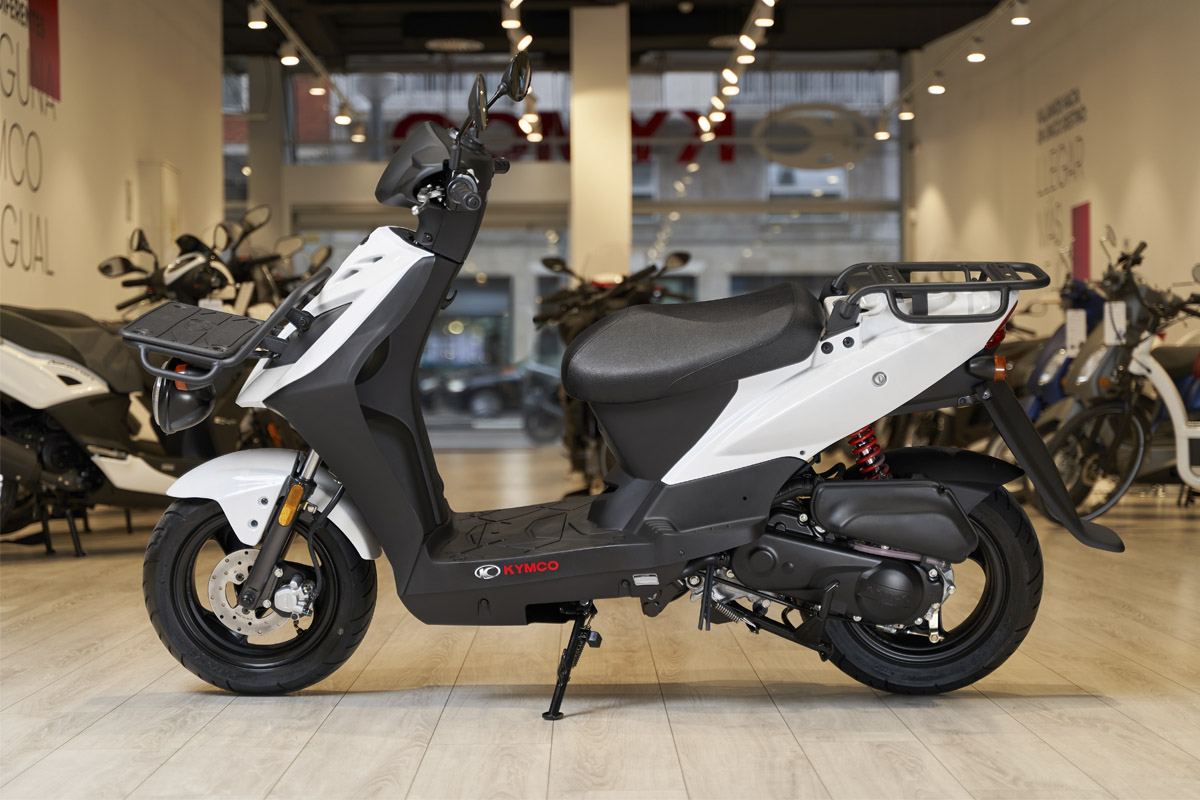
\includegraphics[scale = 0.25]{archivos/KYMCO agility carry.jpg}
    \caption{KYMCO Agility Carry 50 E5.}
    \label{fig:kymco agility carry}
\end{figure}

El motor de la \textbf{\textit{KYMCO Agility Carry 50 E5}} es de los más eficientes que hay en el mercado, se caracteriza por sus bajas emisiones y su poco consumo, tal y como se muestra en la \autoref{tab:comparacion de distintos modelos de ciclomotores de reparto}.

Además de las características que ofrece como equipo de reparto y del valor que añade a los usuarios, la empresa se ve beneficiada por su precio tan competitivo, sin lugar a dudas, su característica más destacable, ya que, por tan solo 1.999 \glssymbol{euro} la empresa puede contar con esta moto como parte de los activos. 

% \paragraph{Estudio del reparto.}
% Todos los cálculos asociados al reparto 
\paragraph{Mantenimiento y robustez}

Este modelo cuenta con un manual de usuario \cite{manualkymcociclomotor} en el que se específica el tratamiento que deben tener, los distintos elementos que componen la moto y la frecuencia con la que deben de cambiarse. 

Como se puede observar en la \autoref{fig:cambio kymco agility 50} el mantenimiento que necesita el ciclomotor no es excesivo, ya que el primer recambio de aceite es necesario después de 1000 \gls{km} o de 3 meses, lo cual nos conduce a la gran durabilidad y robustez con la que cuenta el ciclomotor.

La gran ventaja que ofrece el mantenimiento tardío radica en poder distribuirlos en el tiempo con mayor facilidad para evitar tener toda la flota en el taller y que se necesite de servicios auxiliares o de una segunda flota.

\begin{figure}[h]
    \centering
    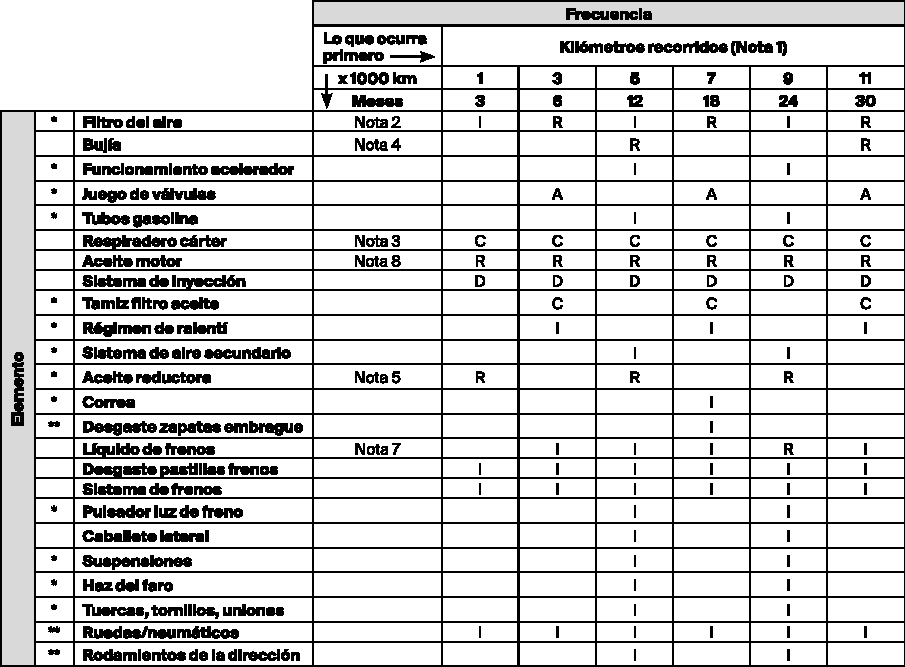
\includegraphics[scale = 1]{archivos/ManualUsuario_AgilityCity50.pdf}
    \caption{Tabla de mantenimiento del ciclomotor  KYMCO Agility Carry 50.}
    \label{fig:cambio kymco agility 50}
\end{figure}

\paragraph{Viabilidad económica}

En el \refanexo{Ciclomotor gasolina 50cc, KYMCO Agility Carry 50} se presentan una serie de cálculos relacionados con la viabilidad económica, en el que se concluye que este modelo es el más barato y el que requiere una menor inversión, cuyo dinero asciende a la cifra de 16.052,70 \glssymbol{euro} el primer año y los siguientes años 4.965,55 \glssymbol{euro}, según la \autoref{tab:Presupuesto motillo Peter}, por consiguiente esto nos da un total de 5 vehículos disponibles para el reparto, lo cual satisfará la demanda.

\paragraph{Conclusiones modelo}
Es el mejor ciclomotor con el que cuenta el mercado, está preparado para satisfacer todas las necesidades que se puedan presentar durante el desempeño de cualquier actividad de reparto, tiene un estilo moderno que combina con la imagen corporativa de cualquier empresa a una relación-calidad precio muy competitiva.
\subsubsection{KYMCO Agility Carry 125}

\paragraph{Descripción general} 
%%El ciclomotor KYMCO Aility Carry 125 es una scooter especializado para el reparto y que además cuenta con unos niveles de emisiones mínimos. Diseñado para dar una respuesta práctica ante cualquier demanda, por lo que tiene dos amplias y robustas parrillas con capacidad de 5Kg de carga para la delantera y hasta 20Kg de carga en la trasera.
Estudiando las consideraciones descritas en \refanexo{anexo_scooter_gasolina}, se ha optado de entre todos los modelos mostrados por la KYMCO Agility Carry 125 en la \autoref{fig:KYMCO Agility Carry 125}. 

\begin{figure}[h]
    \centering
    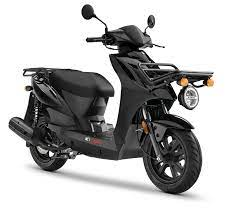
\includegraphics[scale = 0.8]{archivos/KYMCO Agility Carry 125.jpg}
    \caption{KYMCO Agility Carry 125.}
    \label{fig:KYMCO Agility Carry 125}
\end{figure}

Los motivos para elegir este modelo están basados en su especialidad para el reparto y la robustez para este tipo de tareas. La motocicleta es de una cilindrada de 125 \glssymbol{cc}, cuenta con unos niveles de emisiones mínimos y con unas parrillas delantera y trasera con capacidad de carga de hasta 5 \glssymbol{kg} y 20 \glssymbol{kg} respectivamente. Su precio actual en el mercado es de 2.149 \glssymbol{euro}.

La KYMCO Agility Carry 125 cuenta con una autonomía de 250 \glssymbol{km} debido a su depósito con capacidad de 6,5 \glssymbol{litros} y su motor de cuatro tiempos que hace que sea más eficiente. Esta autonomía es más que suficiente para realizar varias jornadas de trabajo sin repostar.

Cuenta con frenos de disco traseros y delanteros para una mayor seguridad, así como suspensiones hidráulicas para una mayor estabilidad, neumáticos de 12 pulgadas para una gran agilidad por ciudad, faros LED y un peso de tan solo 123 \glssymbol{kg}.

%El Barto

% \paragraph{Estudio del reparto.}

%  %Escoger modelo
\paragraph{Mantenimiento y robustez.}
%%Se trata de un modelo muy robusto ya que está concebido para realizar largas jornadas de trabajo.En cuanto al mantenimiento, como cualquier otra motocicleta de 125cc necesita el mantenimiento especificado en el "ANEXO X"(tabla con costes de mantenimiento).

Al ser un modelo muy robusto y concebido para realizar largas jornadas de trabajo, no tendrá tantas averías como otro modelo de motocicleta no especializada, reduciendo los costes en este aspecto.

Una motocicleta necesita mantenimiento en sus frenos, transmisión, ruedas, así como cambios de aceite y revisiones. Esto se estudia en \refanexo{anexo_precio_taller_combustible}, obteniéndose un importe anual de mantenimiento de 239 \glssymbol{euro}.
\paragraph{Viabilidad económica}
%%El coste del primer año de esta motocicleta es de 4.412,42€ y de 2.263,42€ los años sucesivos  según lo calculado en el "ANEXO X".
Para ver si es viable el gasto hay que observar el gasto fijo que supone la adquisición del equipo al completo, y posteriormente el gasto anual entre mantenimiento, seguros y combustible.

Todos los cálculos y estimaciones referentes a la viabilidad económica se pueden encontrar en la \autoref{tab:Presupuesto motocicletas de gasolina}, \refanexo{sub_anexo_calculos_motocicleta}, donde se muestran los presupuestos para ambos modelos de reparto estudiados en el estudio del reparto.

En el primer año, se han de tener en consideración el precio de mercado por unidad de las motocicletas y el número total que se van a comprar, incluyendo también el impuesto de matriculación por cada vehículo adquirido que en este modelo es de 99,77 \glssymbol{euro}. Además de esto, hay que añadir como gasto fijo inicial la adquisición del equipamiento, los cuales se enumeran en la \autoref{consideraciones_preliminares}, considerando en cada caso el número
de personal, o vehículos simultáneos en carretera.

Para los gastos anuales se debe comenzar con el coste del combustible del vehículo y el impuesto de circulación de 8,55 \glssymbol{euro}. Teniendo el precio de la gasolina, obtenido en el \refanexo{anexo_precio_taller_combustible}, se obtiene el gasto semanal y anual relacionado con el combustible. 

Los gastos relacionados con reparaciones o mantenimiento se han fijado en el \refanexo{anexo_precio_taller_combustible}, por lo que se asume un gasto mensual a cada uno.
El coste por seguro fijado es de 265 \glssymbol{euro}, lo cual se multiplicará directamente por el número de vehículos en posesión de manera mensual.

Teniendo todas las consideraciones anteriores descritas, se concluye finalmente el presupuesto necesario en el primer año y posteriores, siendo:

\begin{itemize}
    \item Presupuesto para el primer año del modelo de estudio 1 - 18.058,14 \gls{euro}
    \item Presupuesto anual del modelo de estudio 1 - 5.861,39 \gls{euro}
    \item Presupuesto para el primer año del modelo de estudio 2 - 17.591,70 \gls{euro}
    \item Presupuesto anual del modelo de estudio 2 - 5.394,95 \gls{euro}
\end{itemize}
%%Observando los resultados en \refanexo{anexo_scooter_gasolina}, \refanexo{anexo_precio_taller_combustible} y \autoref{consideraciones_preliminares_seguro} en los que se estudian detalladamente todos los costes que conlleva esta motocicleta se llega a un resultado final de que el coste que implica es de 2.149,00 \glssymbol{euro} de inversión inicial para la compra de la motocicleta y de 2.848,42\glssymbol{euro} anuales en gastos.
\paragraph{Conclusiones modelo.}
%%Es una motocicleta especializada por lo que está garantizado el perfecto cumplimiento de la tarea a realizar y una opción a considerar si no se quiere optar por los vehículos electricos.

Analizando los datos anteriores se concluye que dicha motocicleta es una opción con una gran fiabilidad, desempeño en su tarea y la opción más viable para cubrir largas distancias sin interrupción ni complicaciones. Todo esto a cambio de una mayor inversión inicial y mayor coste anual.

De las opciones que se plantean es el vehículo más seguro y que alcanza la mayor velocidad, por lo que puede realizar un mayor número de repartos, necesitando por ello menos cantidad de ellas. Dada su clasificación L3 dentro de los vehículos puede circular por autovías y autopistas en caso de que sea necesario, facilitando la labor de reparto.

Como principales inconvenientes nos encontramos con que al ser un modelo de combustión conlleva contaminación asociada, tanto medioambiental como en términos de ruido. A diferencia de las opciones eléctricas, el combustible tiene mayor coste que la energía.
\subsection{Eléctricos}
\subsubsection{Askoll eS1}
\label{apartado_moto_electrica}
\paragraph{Descripción general}
%%La motocicleta eléctrica Askoll eS1 es un scooter eléctrico de la empresa pionera en innovación de movilidad eléctrica Askoll de Italia. El scooter de la serie eS es ganador de muchos premios, incluido el Green Prix 2015.El eS1 está equipado con un motor eléctrico de 1.500 vatios con un par de 100 Nm, tiene una velocidad máxima de 45 km / h. El scooter cuenta con una batería de litio extraíble de 2,1 kWh para un alcance de 100 km y La batería se puede cargar en 6 horas.
Estudiando las consideraciones descritas en el \refanexo{anexo_scooter_electrico}, se ha escogido de entre todos los modelos mostrados el Askoll eS1 en la \autoref{fig:Askoll eS1}. 

\begin{figure}[h]
    \centering
    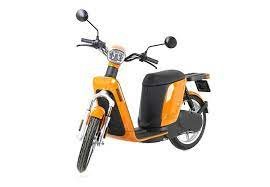
\includegraphics[scale = 0.8]{archivos/askoll es1.jpg}
    \caption{Askoll eS1.}
    \label{fig:Askoll eS1}
\end{figure}

Los motivos para elegir este modelo están basados en su gran autonomía frente a las demás opciones y un tiempo de carga bajo, lo que hace que sea la única opción realista de entre las eléctricas.

El scooter de la serie eS es ganador de muchos premios, incluido el Green Prix 2015. Está equipado con un motor eléctrico de 1.500 \glssymbol{vatios} con un par de 100 \glssymbol{par} y cuenta con una velocidad máxima de 45 \glssymbol{velocidad}. El scooter cuenta con una batería de litio extraíble de 2,1 \glssymbol{kilovatiohora} para un alcance de 100 \glssymbol{km} y la batería se puede cargar en 6 horas.

Cuenta con una autonomía de 100 \glssymbol{km} en ciudad, iluminación \gls{led}, suspensión hidráulica para una mayor estabilidad y frenos de disco para una mayor seguridad. Cuenta con neumáticos de 16 pulgadas para hacerlo más estable frente a las caídas. Un peso de tan solo 72 \glssymbol{kg} la hace muy ligera y manejable en todo tipo de situaciones.

% \paragraph{Estudio del reparto.}
%  %Escoger modelo
\paragraph{Mantenimiento y robustez}
%%Se trata de un modelo muy robusto ya que está concebido para realizar largas jornadas de trabajo. En cuanto al mantenimiento, como cualquier otra motocicleta eléctrica necesita el mantenimiento especificado en el "ANEXO X"(tabla con costes de mantenimiento).
Al ser un modelo eléctrico necesita menos mantenimiento que uno de gasolina, ya que no es necesario el cambio de aceite ni de transmisión. El modelo está construido en materiales de calidad para una mayor robustez.

Una motocicleta eléctrica necesita mantenimiento en sus frenos y ruedas, así como revisiones periódicas. Esto se estudia en el \refanexo{anexo_scooter_electrico}, obteniéndose un importe anual de mantenimiento de 126 \glssymbol{euro}.

\paragraph{Viabilidad económica}
%%El coste del primer año de esta motocicleta es de 3.348,94€ y de 663,94€ los años sucesivos  según lo calculado en el "ANEXO X".

%%Observando los resultados en \refanexo{anexo_scooter_electrico} y \autoref{consideraciones_preliminares_seguro} en los que se estudian detalladamente todos los costes que conlleva esta motocicleta se llega a un resultado final de que el coste que implica es de 2.685,00\glssymbol{euro} de inversión inicial para la compra de la motocicleta y de 753,44\glssymbol{euro} anuales en gastos.

Para ver si es factible el gasto hay que observar el gasto fijo que supone la adquisición del equipo al completo, y posteriormente el gasto anual entre mantenimiento, seguros y recargas. 

Todos los cálculos y estimaciones referentes a la viabilidad económica se pueden encontrar en la \autoref{tab:Estudio presupuestos modelo Askoll eS1}, \refanexo{sub_anexo_calculos_motocicleta_eléctrica}, donde se muestran los presupuestos para ambos modelos de reparto analizados en el estudio del reparto.

En el primer año, se han de tener en consideración el precio de mercado por unidad de las motocicletas eléctricas y el número total que se van a comprar, pues el impuesto de matriculación unitario es de 27,85 \glssymbol{euro}. Además de esto, hay que añadir como gasto fijo inicial la adquisición del equipamiento, los cuales se enumeran en la \autoref{consideraciones_preliminares}, considerando en cada caso el número de personal, o vehículos simultáneos en carretera.

Para los gastos anuales se debe comenzar con el coste de recarga del vehículo y el impuesto de circulación de 8,55 \glssymbol{euro}. Teniendo el precio de la luz, obtenido en el \refanexo{anexo_precio_taller_combustible} y el número de recargas semanales totales, junto con la capacidad de una batería, se obtiene el gasto semanal y anual relacionado con la recarga.

Los gastos relacionados con reparaciones o mantenimiento se han fijado en el \refanexo{anexo_scooter_electrico}, por lo que se asume un gasto mensual a cada uno. 

El coste por seguro fijado es de 265 \gls{euro}, lo cual se multiplicará directamente por el número de vehículos en posesión de manera mensual.

Teniendo todas las consideraciones anteriores descritas, se concluye finalmente el presupuesto necesario en el primer año y posteriores, recogidos en la \autoref{tab:Estudio presupuestos modelo Askoll eS1}, siendo:

\begin{itemize}
    \item Presupuesto para el primer año del modelo de estudio 1 - 30.475,64 \gls{euro}
    \item Presupuesto anual del modelo de estudio 1 - 5.107,09 \gls{euro}
    \item Presupuesto para el primer año del modelo de estudio 2 - 23.977,50 \gls{euro}
    \item Presupuesto anual del modelo de estudio 2 - 4.034,65 \gls{euro}
\end{itemize}

\paragraph{Conclusiones modelo.}
%%Es un modelo válido para la tarea debido a sus características y el bajo coste de mantenimiento.

Analizando los datos anteriores se concluye que dicha motocicleta es una opción con una gran autonomía, desempeño en su tarea y la opción más viable para cubrir largas distancias con pocas interrupciones. Todo esto teniendo en cuenta que tendrá que parar a recargarse cada 100 \glssymbol{km} para poder seguir con su labor de reparto.

De las opciones que se plantean es el vehículo eléctrico que alcanza la mayor velocidad y cuenta con la mayor autonomía de ellos, por lo que puede realizar un mayor número de repartos, necesitando por ello menos cantidad de ellas. Dada su clasificación dentro de los vehículos, no puede circular por autovías y autopistas en caso de que sea necesario, siendo este un factor a tener en cuenta para repartos.

Al ser un modelo de eléctrico no conlleva una contaminación, tanto medioambiental como en términos de ruido. A diferencia de las opciones de gasolina, la energía es más barata.
%\subsubsection{Bicicletas eléctricas}
%\paragraph{Descripción general}
% \paragraph{Estudio del reparto.}
%  %Escoger modelo
% \paragraph{Mantenimiento y robustez.}
% \paragraph{Viabilidad económica}
% \paragraph{Conclusiones modelo.}

\paragraph{Consideraciones previas}

Esto debe ir como ANEXO, las bicis son considerados vehículos HÍBRIDOS, no eléctricos

Las bicicletas de pedaleo deben de llevar siempre pedales y no pueden funcionar con un acelerador, por lo que es totalmente ilegal conducir por la vía pública las ``mini-bicicleta" sin pedales, según recoge el BOE y la normativa de circulación.  Según la normativa vigente, excluiremos del estudio este tipo de vehículo.

Las bicicletas eléctricas propiamente hablando son reconocidas como ``ciclo de pedaleo asistido" según el BOE N.º 124\cite{boe124}, lo que implica que aunque tienen motor eléctrico auxiliar, no pueden ser propulsadas exclusivamente haciendo uso del mismo, por lo que son vehículos híbridos entre eléctrico y manual.

\paragraph{Modelo F.Lli Schiano E-Moon}

Actualmente, una de las mejores bicicletas eléctricas del mercado calidad-precio que cumple con todas las normativas vigentes es el modelo F.Lli Schiano E-Moon, que está a la venta por 729 \glssymbol{euro}.

Respecto a sus características, posee un motor delantero ANANDA M129F de 250 \glssymbol{vatios} de potencia y 36 \glssymbol{voltios}, que permite alcanzar velocidades de hasta 25 \glssymbol{velocidad}. Presenta una batería de litio GREENWAY YJ145 36\glssymbol{voltios} 13\glssymbol{amperiohora} 468\glssymbol{vatiohora}, con una vida útil de entre 4 y 6 años y una autonomía de hasta 120 \glssymbol{km} con 6 horas de carga completa. 

Su sistema de frenado es V-Brake en las ruedas delantera y trasera, ambos neumáticos son Kenda de 26 pulgadas. El cuerpo de la bicicleta no es plegable, es de una aleación de aluminio resistente, aunque no ligera (25 \glssymbol{km}). Consta de una caja de cambios Shimano Tourney TY21 de 7 velocidades, un timbre, una luz delantera y otra trasera. 
Cumple todos los requisitos para ser considerada una bicicleta eléctrica:

\begin{itemize}
\item Tener dos ruedas, tal como considera El Real Decreto 2822/1998, de 23 de diciembre, que aprueba el Reglamento General de Vehículos.\cite{boe2822}
\item Contar con un motor eléctrico cuya potencia máxima no exceda los 250 \glssymbol{vatios}.
\item Alcanzar una velocidad máxima asistida de 25 \glssymbol{velocidad}.
\item El motor ha de encender con el pedaleo y apagarse al llegar a 25 \glssymbol{velocidad} o cuando el pedaleo cese.
\end{itemize}

Al cumplir todos los requisitos anteriores no es necesario seguro obligatorio, matrícula, tarjeta de inspección técnica, casco ni permiso de conducción para circular por las vías públicas. No obstante, sí es necesario que el vehículo cuente con:


\begin{itemize}
\item Doble sistema de frenado, un freno para la rueda delantera y otro para la trasera.
\item Timbre. 
\item Luces de posición. La luz delantera debe ser de color blanco y la posterior de color rojo.
\item Señalización trasera.
\end{itemize}

Todas las especificaciones numeradas están incluidas en el modelo seleccionado.

Las bicicletas eléctricas no tienen restricciones relevantes de circulación en la vía pública, pueden usar los carriles bici o la carretera en su defecto. Además, si fuese necesario pueden circular por el arcén en autovías.

\paragraph{Viabilidad del modelo}

Tal como se recoge en el plano 3 del Anexo “X”, el rango de alcance de los repartos es de 6 \glssymbol{km} poniendo como centro la localización de la sede.

Haciendo uso de los cálculos recogidos en el anexo “X” son necesarias unas 8 bicicletas eléctricas, las cuales se usarán durante todo el día y se recargarán por la noche, en el horario de cierre del negocio (24:00-9:00).

Suponiendo una revisión mensual de mantenimiento, el precio de la luz en el horario en el que se producirá la recarga de los vehículos, el coste de adquisición de los vehículos recogidos en la tabla "x". 

El coste de adquisición de los vehículos, junto y el resto de servicios requeridos por los mismos, supondría \glssymbol{euro}, tal como se expresa en la ecuación "x"

En los años siguientes, el coste en vehículos sería de aproximadamente ...\glssymbol{euro}.

De este modo, se estima que en 10 años la empresa habrá invertido ... \glssymbol{euro} en los vehículos, incluido mantenimiento, reparaciones y recargas.

La empresa ha de invertir un coste de ... bastante primer año de adquisición de los vehículos es de …. € y él anualmente se gastarían … \glssymbol{euro}.


SUPUESTA TABLA:

Precio estimado de la luz en el tramo horario 24:00-6:00 con base en los datos de los últimos meses en ese tramo horario: 0.2645 \glssymbol{euro}/\glssymbol{kilovatiohora}

Precio mantenimiento general bicicleta eléctrica en Feuvert:44,95 \glssymbol{euro}/anuales



En vista de los resultados económicos y de buena imagen de la empresa hacia el consumidor debido al método de reparto ecológico, es evidente que es una buena opción a tener en cuenta entre los distintos vehículos del mercado. No obstante, ha de considerarse que para ciertos trayectos próximos a los 6 km o que impliquen el uso de algún tramo de autovía, no es aconsejable el uso de este modelo eléctrico por seguridad del transportista y/o por exceso del tiempo de reparto deseado. Asimismo, las opciones de estacionamiento de bicicletas son limitadas, semáforos, farolas y barandillas no están permitidas, por lo que se ha de localizar un parking de bicicletas o estacionarlas del mismo modo que una moto convencional (en este último método, sería necesario también el uso de una cadena especial).

MIS fuentes:
https://www.feuvert.es/movilidad-bicis-mantenimiento/r132.html
https://tarifaluzhora.es/
https://www.almaskater.com/bicicletas-electricas-baratas/
https://www.boe.es/boe/dias/2014/05/22/pdfs/BOE-A-2014-5399.pdf

\subsubsection{Infiniton CITYJam Pro}
\label{apartado_patinetes}
\paragraph{Descripción general}

Estudiando las consideraciones descritas en el \refanexo{anexo_patienete eléctrico}, se ha optado de entre todos los modelos por la Infiniton CITYJam Pro \cite{infinitoncityjam}, mostrado en la \autoref{fig:Infinity CityJam}.

\begin{figure}[h]
    \centering
    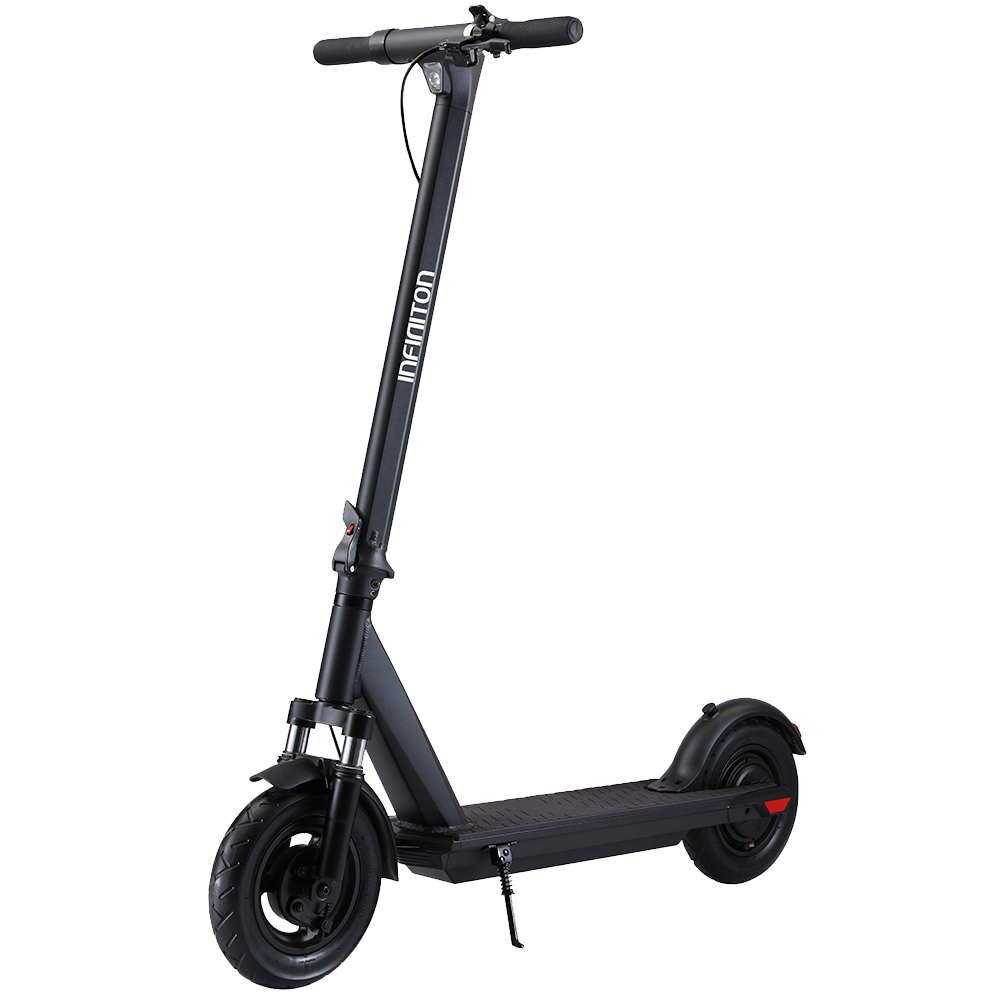
\includegraphics[scale = 0.2]{archivos/cityjam-pro-negro.jpg}
    \caption{Infiniton CITYJam Pro.}
    \label{fig:Infinity CityJam}
\end{figure}

Los motivos para elegir este modelo se fundamentan en su larga autonomía frente a los demás, y su capacidad en batería, permitiendo cargas más económicas y espaciadas en el tiempo. No se han tenido en consideración la inclinación del terreno o el peso máximo, dado que el rango de destino, terreno de la ciudad, y tipos de pedidos no suponen la  importancia necesaria.

La Infiniton CITYJam Pro tiene una autonomía de entre 40-45 \glssymbol{km} de distancia gracias a su batería de 350 \glssymbol{vatiohora}. Al igual que otros modelos en el mercado, cuenta con un sistema de recarga de energía cuando se frena, permitiendo prolongar la vida de cada carga.

Dispone de mucha estabilidad y durabilidad gracias al uso de acero resistente en su fabricación, junto con tres sistemas de frenos distintos y luces frontales y traseras para garantizar la seguridad del usuario.

La potencia que ofrece este modelo permite transportar cargas de hasta 100 \glssymbol{kg}, siendo suficiente para transportar al repartidor junto con el pedido.

\paragraph{Mantenimiento y robustez}

El patinete está fabricado con los materiales necesarios para soportar el día a día frente a un uso de ciudad. Además de ello, cuenta con un grado de protección IP54, controlado por la norma internacional CEI 60529 \cite{une60529}, capaz de soportar lluvia y polvo sin ningún tipo de problema.

El mantenimiento \cite{mantenimientopatinete} es más sencillo y económico comparado con un coche o una moto. Se recomienda emplear siempre piezas originales y no utilizar cargadores distintos al original. La limpieza del vehículo se puede realizar con ayuda de un trapo y cepillo, evitando el uso de mangueras de presión localizados en lavaderos de coches. 

Por otro lado, el modelo que estudiamos tiene ruedas de diez pulgadas, por lo que su durabilidad frente al desgaste va a ser alta. En caso de daño o fin de su vida útil, se pueden sustituir manualmente con recambios, sin necesidad de acudir a un taller especializado.

En referencia al sistema electrónico o la batería, se ha de evitar manipularlo, y en caso de avería llevarlo a un taller especializado. Las reparaciones dependen del daño y del taller al que se acuda, pero su precio no excede el de una avería de moto u otros tipos de vehículos.

Además de todo lo anterior, tal y como se indica en el \refanexo{anexo_precio_taller_combustible}, se incluye una cantidad fija de ahorro para caso de siniestro y sustitución de patinete.

\paragraph{Viabilidad económica}

Para ver si es aceptable el gasto hay que observar el gasto fijo que supone la adquisición del equipo al completo, y posteriormente el gasto anual entre mantenimiento, seguros y recargas. 

Todos los cálculos y estimaciones referentes a la viabilidad económica se pueden encontrar en la \autoref{tab: analisis_presupuestos_patienetes}, \refanexo{sub_anexo_calculos_patinete}, donde se muestran los presupuestos para ambos modelos de reparto estudiados en el estudio del reparto.

En el primer año, se han de tener en consideración el precio de mercado por unidad de los patinetes y el número total de patinetes que se van a comprar, según el \refanexo{anexo_calculos_sobre_vehiculos} son necesarios un total de 20 patinetes según la hipótesis de reparto de 5 \glssymbol{km} y 16 según la hipótesis de pedidos dobles. Además de esto, hay que añadir como gasto fijo inicial la adquisición del equipamiento, los cuales se enumeran en la \autoref{consideraciones_preliminares}, considerando en cada caso el número de empleados, o vehículos simultáneos en carretera que en este modelo serán 8 y 7, respectivamente.

Para los gastos anuales se debe comenzar con el coste de recarga del vehículo. Teniendo el precio de la luz, obtenido en el \refanexo{anexo_precio_taller_combustible} y el número de recargas semanales totales, junto con la capacidad de una batería, se obtiene el gasto semanal y anual relacionado con la recarga.

Los gastos relacionados con reparaciones o mantenimiento se han fijado en el \refanexo{anexo_precio_taller_combustible}, por lo que se asume un gasto mensual a cada uno. 

El coste por seguro fijado es de 35 \gls{euro}, lo cual se multiplicará directamente por el número de vehículos en posesión de manera mensual.

Teniendo todas las consideraciones anteriores descritas, se concluye finalmente el presupuesto necesario en el primer año y posteriores, siendo:

\begin{itemize}
    \item Presupuesto para el primer año del modelo de estudio 1 - 12.323,53 \gls{euro}
    \item Presupuesto anual del modelo de estudio 1 - 3.873,05 \gls{euro}
    \item Presupuesto para el primer año del modelo de estudio 2 - 9.926,05 \gls{euro}
    \item Presupuesto anual del modelo de estudio 2 - 3.096,81 \gls{euro}
\end{itemize}


\paragraph{Conclusiones modelo.}

Analizando los datos obtenidos, se llega a la conclusión que en cuestiones económicas, el patinete eléctrico es una de las opciones más baratas del mercado. A pesar de ser necesario una flota grande inicial para disponer siempre de un vehículo operativo, el coste sigue siendo menor que otras alternativas.

El coste energético es proporcional al precio de la electricidad, aunque comparado con la gasolina sigue siendo una alternativa eficiente y económica.

Los inconvenientes de este modelo de transporte son por un lado la seguridad del conductor, debido a lo vulnerable que es a los accidentes en carretera y condiciones meteorológicas, y por otro lado la cantidad necesaria de vehículos para garantizar el correcto funcionamiento del servicio, debido a que implica la posesión de las tomas de corriente suficientes para realizar múltiples cargas simultaneas.
\subsection{Comparativa entre los modelos estudiados}
A modo de resumen, la \autoref{tab:resumen_final}
incluye el número de vehículos necesarios para cada una de las opciones estudiadas a lo largo de esta sección, junto con sus precios actuales en el mercado, que definirá en gran medida la inversión inicial. Asimismo, se recogen el número de vehículos que han de estar simultáneamente en carretera, lo cual delimita la cantidad de recurso humano que debe invertir la empresa dependiendo del modelo elegido.

% Tabla
\begin{table}[H]
\centering
\begin{tabular}{l|c|c|c|c|}
\cline{2-5}
 & \multicolumn{1}{l|}{Ciclomotor} & \multicolumn{1}{l|}{Motocicleta} & \multicolumn{1}{l|}{Patinete eléctrico} & \multicolumn{1}{l|}{Motocicleta eléctrica} \\ \hline
\multicolumn{1}{|l|}{Coste  unitario vehículo (\glssymbol{euro})} & 1.999,00 & 2.149,00 & 376,62 & 2.685,00 \\ \hline
\multicolumn{1}{|l|}{\begin{tabular}[c]{@{}l@{}}N º vehículos totales \\ necesarios caso 1\end{tabular}} & 5 & 5 & 20 & 9 \\ \hline
\multicolumn{1}{|l|}{\begin{tabular}[c]{@{}l@{}}N º vehículos totales \\ necesarios caso 2\end{tabular}} & 5 & 5 & 16 & 7 \\ \hline
\multicolumn{1}{|l|}{\begin{tabular}[c]{@{}l@{}}N º vehículos simultáneos \\ en carretera, caso 1\end{tabular}} & 5 & 5 & 8 & 5 \\ \hline
\multicolumn{1}{|l|}{\begin{tabular}[c]{@{}l@{}}N º vehículos simultáneos\\  en carretera, caso 2\end{tabular}} & 5 & 5 & 7 & 5 \\ \hline
\end{tabular}
\caption{Resumen número de vehículo imprescindibles según cada modelos estudiados}
\label{tab:resumen_final}
\end{table}
Una vez analizados diversos vehículos factibles para el reparto de comida a domicilio, se han realizado también la \autoref{fig:comparativa_caso_1} donde se comparan los costes económicos de las opciones estudiadas para el supuesto de que cada reparto incluya un único pedido y la \autoref{fig:comparativa_caso_2}, referente a la hipótesis de los pedidos dobles.

\begin{figure}[h]
    \centering
    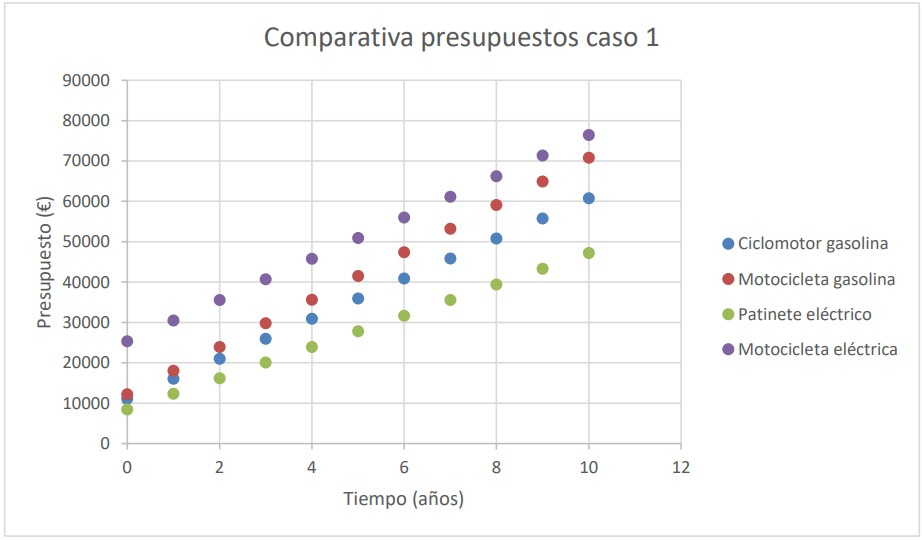
\includegraphics[scale = 0.4]{archivos/Comparativa_presupuestos_caso_1.jpeg}
    \caption{Comparación de presupuestos de los vehículos para repartos individuales}
    \label{fig:comparativa_caso_1}
\end{figure}

\begin{figure}[h]
    \centering
    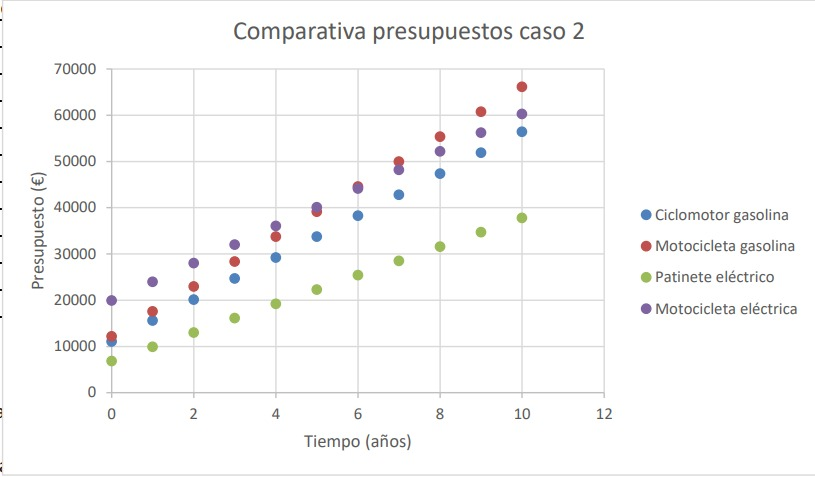
\includegraphics[scale = 0.4]{archivos/Comparativa_presupuestos_caso_2.jpeg}
    \caption{Comparación de presupuestos de los vehículos para repartos dobles}
    \label{fig:comparativa_caso_2}
\end{figure}

Se observa que la \autoref{fig:comparativa_caso_1}, las motocicletas eléctricas, destacan como vehículo más caro, aunque ciertamente, la recta que define sus presupuestos tiende a aplanarse y abaratarse en un periodo de tiempo mayor. No obstante, si se observa la \autoref{fig:comparativa_caso_2}, apenas hay diferencia de precio entre la motocicleta eléctrica y las de gasolina.



Económicamente, la opción más rentable son los patinetes eléctricos en ambas figuras y la peor opción es la motocicleta de gasolina, seguida de la motocicleta eléctrica. No obstante, partiendo de la premisa inicial de cubrir un radio de 6 \glssymbol{km} desde el establecimiento que impone la empresa \textit{DELICIOUS BURGER S.A.}; es evidente que el uso de patines eléctricos para entregar pedidos a 5 o 6 km de distancia no es lo ideal, además de tener que atravesar un tramo de autovía (prohibido por ley para este tipo de vehículos), el cliente recibiría su pedido con retardo y frío. Por consiguiente, se ha decidido indagar una alternativa a usar un único vehículo.

\subsection{Opción óptima}
\subsubsection{Justificación de la elección}

En el \refanexo{anexo_scooter_electrico} y en el \refanexo{anexo_patienete eléctrico} se ha debatido la mejor opción dentro de la gama de motocicletas eléctricas y patinetes eléctricos, respectivamente. En consecuencia, se plantea una alternativa eficiente y coherente que cohesiona a la perfección la autonomía que proporciona el modelo de motocicleta Askoll eS1, con el precio competitivo de los patinetes Infiniton CITYJam Pro, cuyas características se encuentran detalladas en la
\autoref{apartado_moto_electrica} y en la \autoref{apartado_patinetes} de esta \autoref{Estudio de los modelos}.


Tomando en consideración que el reparto de los pedidos es homogéneo en todas las franjas horarias, el radio de alcance máximo es de 6 \glssymbol{km} que aparece en el \hyperref[plano:radio]{\hyperlink{plano:radio}{Plano 3}} del \refanexo{anexo_planos}, y la longitud de los pedidos contando ida y vuelta de media oscila entre los 5 y los 7,5 \glssymbol{km}; se puede suponer que la longitud de los recorridos también posee cierta uniformidad. Por ello, se estima que el número de pedidos que se han de repartir en un radio de 4 a 6 \glssymbol{km} desde el establecimiento, supondrá a lo sumo un 33 \% de los mismos.

La solución que se plantea es que las motocicletas eléctricas cubran ese porcentaje de pedidos lejanos en todos y cada uno de los tramos horarios estudiados, mientras que los pedidos de corto alcance se realicen en patinetes. De este modo, se elimina el problema que presentan los patinetes al no poder alcanzar todas las áreas donde se debían realizar las entregas, al mismo tiempo que se mejora el tiempo de entrega en pedidos cortos porque los patinetes no necesitan ser estacionados, pueden acompañar a su conductor hasta la misma puerta del cliente.

\subsubsection{Estudio del reparto}
Una motocicleta eléctrica del modelo Askoll eS1 es capaz de realizar unos 100 \glssymbol{km} a carga completa, lo que equivale a 20 pedidos, suponiendo que los repartos tienen una duración media de 5 \glssymbol{km}, o 13 pedidos si se suponen 7,5 \glssymbol{km}. Realizando los mismos cálculos que en el \autoref{anexo_calculos_sobre_vehiculos}, pero reduciendo el número de pedidos a realizar en cada tramo horario, se obtiene que son necesarias aparentemente unos 18 patinetes para la primera hipótesis contemplada (repartos individuales de 5 km) y 16 patinetes para el caso de realizar repartos dobles de 7,5 \glssymbol{km} de ida y vuelta, según la \autoref{tab: analisis_detallado_patinete_5km_22} y la \autoref{tab: analisis_detallado_patinete_7,5km_22}.

\begin{table}[H]
\centering
\begin{tabular}{l|c|c|c|c|}
\cline{2-5}
 & \begin{tabular}[c]{@{}c@{}}TRAMO \\ HORARIO 1\end{tabular} & \begin{tabular}[c]{@{}c@{}}TRAMO \\ HORARIO 2\end{tabular} & \begin{tabular}[c]{@{}c@{}}TRAMO \\ HORARIO 3\end{tabular} & \begin{tabular}[c]{@{}c@{}}TRAMO \\ HORARIO 4\end{tabular} \\ \cline{2-5} 
 & \begin{tabular}[c]{@{}c@{}}Lunes-Jueves \\ (9:00-20:00)\end{tabular} & \begin{tabular}[c]{@{}c@{}}Lunes-Jueves \\ (20:00-0:00)\end{tabular} & \begin{tabular}[c]{@{}c@{}}Viernes-Domingo \\ (9:00-20:00)\end{tabular} & \begin{tabular}[c]{@{}c@{}}Viernes-Domingo \\ (20:00-1:00)\end{tabular} \\ \hline
\multicolumn{1}{|l|}{Nº pedidos} & 30 & 40 & 44 & 90 \\ \hline
\multicolumn{1}{|l|}{\begin{tabular}[c]{@{}l@{}}Distancia total a \\ recorrer \glssymbol{km}\end{tabular}} & 150 & 200 & 220 & 450 \\ \hline
\multicolumn{1}{|l|}{\begin{tabular}[c]{@{}l@{}}Tiempo total de \\ reparto \glssymbol{minuto} \end{tabular}} & 660 & 240 & 660 & 300 \\ \hline
\multicolumn{1}{|l|}{\begin{tabular}[c]{@{}l@{}}Tiempo estimado \\ por pedido (\glssymbol{minuto}/pedido)\end{tabular}} & 20 & 20 & 20 & 20 \\ \hline
\multicolumn{1}{|l|}{\begin{tabular}[c]{@{}l@{}}Nº pedidos realizables \\ por vehículo\end{tabular}} & 33 & 12 & 33 & 15 \\ \hline
\multicolumn{1}{|l|}{\begin{tabular}[c]{@{}l@{}}Nº vehículos simultáneos \\ necesarios\end{tabular}} & 1 & 4 & 2 & 6 \\ \hline
\multicolumn{1}{|l|}{Nº de turnos de vehículos} & 4 & 8 & 3 & 2 \\ \hline
\multicolumn{1}{|l|}{\begin{tabular}[c]{@{}l@{}}Nº vehículos totales \\ necesarios\end{tabular}} & 4 & 8 & 6 & 12 \\ \hline
\end{tabular}
\caption{Análisis detallado del reparto en patinete con viajes de 5 \glssymbol{km}.}
\label{tab: analisis_detallado_patinete_5km_22}
\end{table}



\begin{table}[H]
\centering
\begin{tabular}{l|c|c|c|c|}
\cline{2-5}
 & \begin{tabular}[c]{@{}c@{}}TRAMO \\ HORARIO 1\end{tabular} & \begin{tabular}[c]{@{}c@{}}TRAMO \\ HORARIO 2\end{tabular} & \begin{tabular}[c]{@{}c@{}}TRAMO \\ HORARIO 3\end{tabular} & \begin{tabular}[c]{@{}c@{}}TRAMO \\ HORARIO 4\end{tabular} \\ \cline{2-5} 
 & \begin{tabular}[c]{@{}c@{}}Lunes-Jueves \\ (9:00-20:00)\end{tabular} & \begin{tabular}[c]{@{}c@{}}Lunes-Jueves \\ (20:00-0:00)\end{tabular} & \begin{tabular}[c]{@{}c@{}}Viernes-Domingo \\ (9:00-20:00)\end{tabular} & \begin{tabular}[c]{@{}c@{}}Viernes-Domingo \\ (20:00-1:00)\end{tabular} \\ \hline
\multicolumn{1}{|l|}{Nº pedidos dobles} & 7 & 12 & 17 & 47 \\ \hline
\multicolumn{1}{|l|}{\begin{tabular}[c]{@{}l@{}}Distancia total a \\ recorrer (\glssymbol{km})\end{tabular}} & 52,5 & 90 & 127,5 & 352,5 \\ \hline
\multicolumn{1}{|l|}{\begin{tabular}[c]{@{}l@{}}Tiempo total de \\ reparto doble (\glssymbol{minuto})\end{tabular}} & 660 & 240 & 660 & 300 \\ \hline
\multicolumn{1}{|l|}{\begin{tabular}[c]{@{}l@{}}Tiempo estimado por \\ pedido doble (\glssymbol{minuto}/pedido)\end{tabular}} & 32,5 & 32,5 & 32,5 & 32,5 \\ \hline
\multicolumn{1}{|l|}{\begin{tabular}[c]{@{}l@{}}Nº pedidos dobles \\ realizables por vehículo\end{tabular}} & 20 & 7 & 20 & 9 \\ \hline
\multicolumn{1}{|l|}{\begin{tabular}[c]{@{}l@{}}Nº vehículos simultáneos \\ necesarios\end{tabular}} & 1 & 2 & 1 & 6 \\ \hline
\multicolumn{1}{|l|}{Nº de turnos de vehículos} & 2 & 2 & 4 & 2 \\ \hline
\multicolumn{1}{|l|}{\begin{tabular}[c]{@{}l@{}}Nº vehículos totales \\ necesarios\end{tabular}} & 2 & 4 & 4 & 12 \\ \hline
\end{tabular}
\caption{Análisis detallado del reparto en patinete con viajes de 7,5 \glssymbol{km}.}
\label{tab: analisis_detallado_patinete_7,5km_22}
\end{table}

Seguidamente, se analizan mediante gráficas el número de patinetes necesarios para las franjas horarias donde se produce el \gls{cuello de botella}, es decir, los fines de semana. Todo esto dependerá sustancialmente del tiempo que dura la recarga de los patinetes.

En la \autoref{fig:patinetes_caso1_2} aparecen representados en azul los 3 turnos de 2 patinetes vehículos cada uno, así como los 2 turnos de 6 patinetes por la tarde (color verde). Según el tiempo de recarga de las baterías, los dos patinetes del primer turno de la mañana se pueden emplear en el segundo turno de vehículos de la tarde. En consecuencia, para el primer caso estudiado solo son necesarios 16 patinetes en total.

\begin{figure}[H]
    \centering
    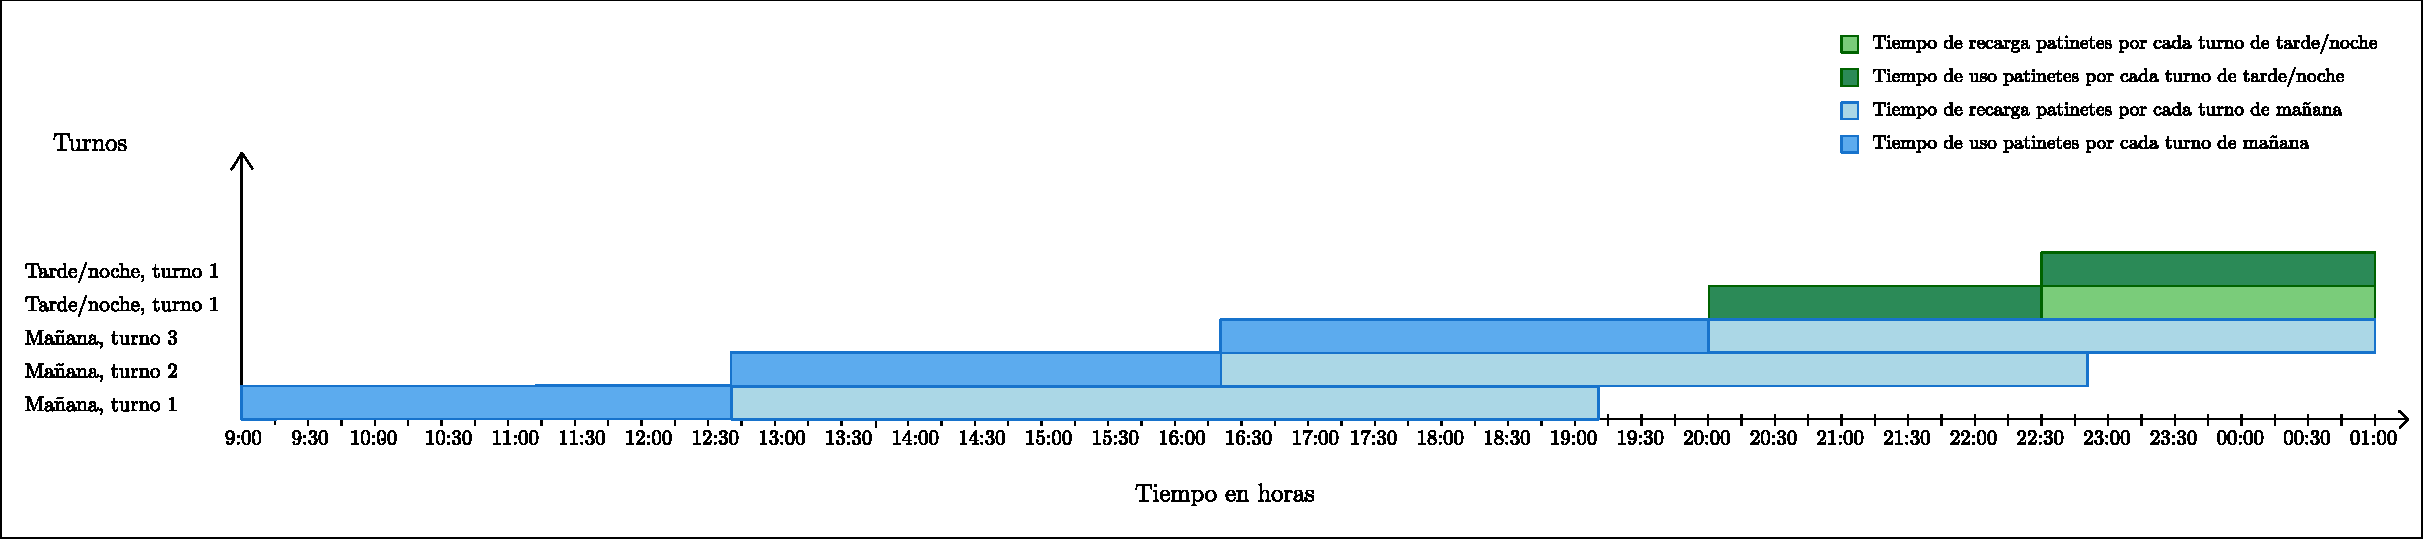
\includegraphics[width= \textwidth, height=12em]{archivos/caso2_patinetes.pdf}
    \caption{Representación turnos minorados de patinetes en viajes de 5 \glssymbol{km}.}
    \label{fig:patinetes_caso1_2}
\end{figure}

Igualmente, en la \autoref{fig:patinetes_caso2_2} se observa que 2 de los patinetes del turno de mañana se pueden recargar y utilizar en el horario posterior, por lo que para esa hipótesis solo son necesarios 14 patinetes.

\begin{figure}[H]
    \centering
    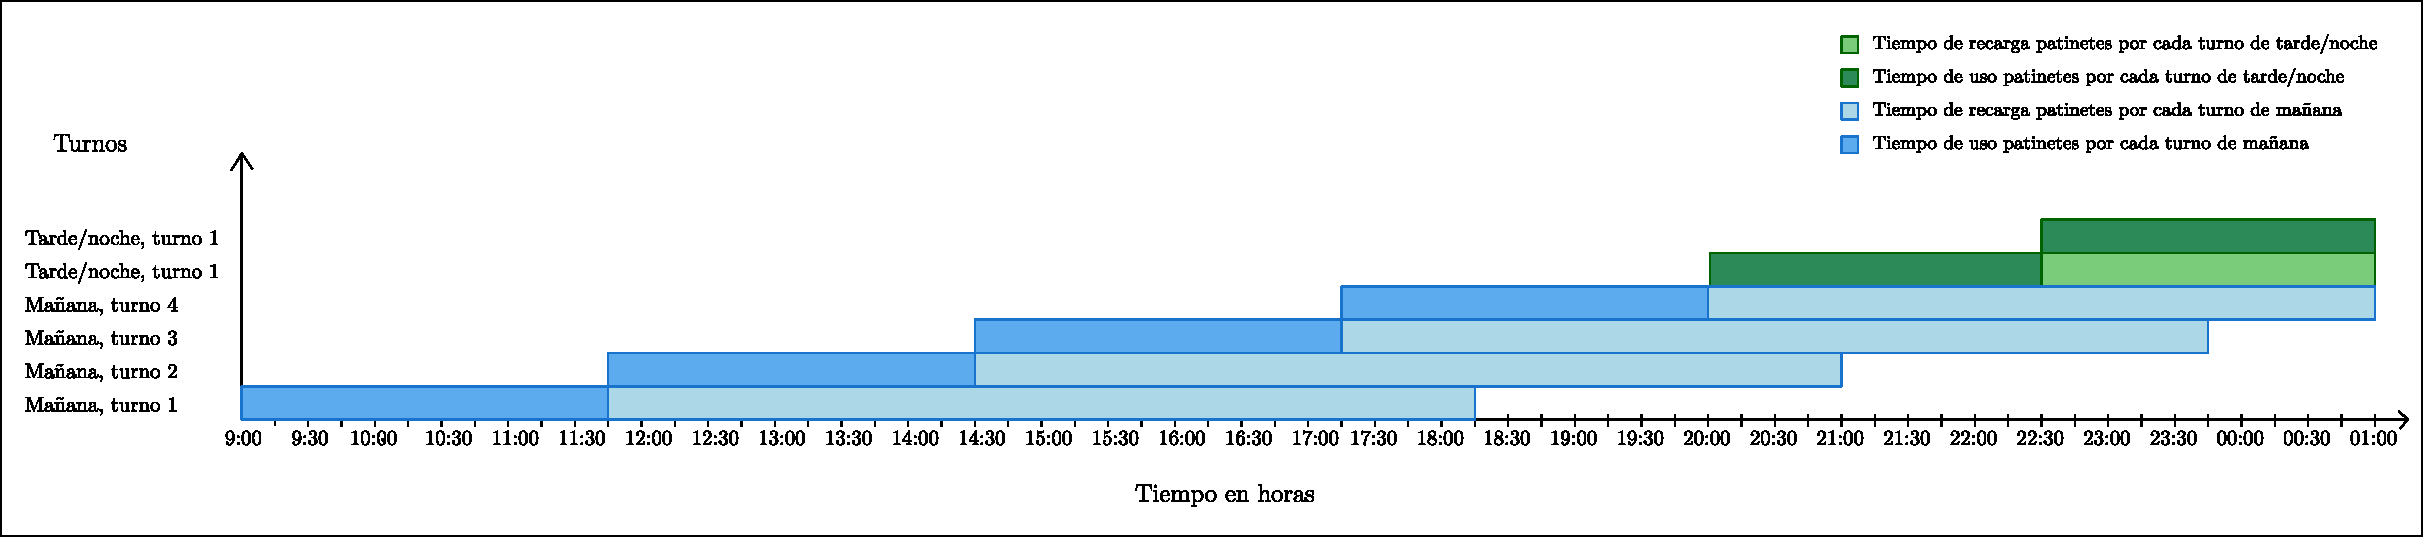
\includegraphics[width= \textwidth, height=12em]{archivos/caso1_patinetes.pdf}
    \caption{Representación turnos minorados de patinetes en viajes de 7,5 \glssymbol{km}.}
    \label{fig:patinetes_caso2_2}
\end{figure}

\subsubsection{Presupuestos}
Finalmente, para hallar el presupuesto de esta opción híbrida se deben tener en cuenta diversos factores. 

Como se ha mencionado anteriormente, se supone  que las motocicletas cubren el 33\% de los repartos, por ello los días entre semana se empleará una motocicleta para todo el día, mientras que en los fines de semana se usará una motocicleta en el turno de mañana y en el turno de tarde se ha de emplear la motocicleta del turno anterior además de otra a plena carga.

Respecto a los cálculos se ha de sumar el número de patinetes y sus costes asociados, así como los dos patinetes y sus respectivos costes, todo queda recogido en la \autoref{tab: analisis_presupuestos_patinetes_y_motos}. En estos cálculos se han empleado datos de la \autoref{tabla:tabla_datos_comunes}, de la \autoref{tab: analisis_presupuestos_patienetes} y de la \autoref{tab:Estudio presupuestos modelo Askoll eS1} debido a que estos modelos ya se han analizado en detalle en el \autoref{anexo_calculos_sobre_vehiculos}.

\begin{table}[H]
\centering
\begin{tabular}{|l|c|}
\hline
Nº patinetes necesarios caso 1 & 16 \\ \hline
Nº patinetes necesarios caso 2 & 14 \\ \hline
Nº motocicletas necesarias en ambos casos & 2 \\ \hline
Nº recargas semanales patinetes caso 1 & 102 \\ \hline
Nº recargas semanales patinetes caso 2 & 72 \\ \hline
Nº recargas semanales motocicletas caso 1 & 10 \\ \hline
Nº recargas semanales motocicletas caso 2 & 10 \\ \hline
Presupuesto anual en recargas caso 1 (\glssymbol{euro}) & 330,01 \\ \hline
Presupuesto anual en recargas caso 2 (\glssymbol{euro}) & 268,90 \\ \hline
Presupuesto para vehículos primer año caso 1 (\glssymbol{euro}) & 16.536,67 \\ \hline
Presupuesto para vehículos primer año   caso 2 (\glssymbol{euro}) & 15.362,72 \\ \hline
Presupuesto para vehículos anual  caso 1 (\glssymbol{euro}) & 4.205,91 \\ \hline
Presupuesto para vehículos anual caso 2 (\glssymbol{euro}) & 3.785,20 \\ \hline
Presupuesto en vehículos a 10 años, caso 1 (\glssymbol{euro}) & 54.389,9 \\ \hline
Presupuesto en vehículos a 10 años, caso 2 (\glssymbol{euro}) & 49.429,53 \\ \hline
\end{tabular}
\caption{Análisis de los presupuestos opción óptima.}
\label{tab: analisis_presupuestos_patinetes_y_motos}
\end{table}


% 3.4.4. Ventajas y desventajas
Las ventajas que proporciona este modelo híbrido de reparto usando 2 vehículos 100\% son diversas. Cabe destacar que los patinetes eléctricos en repartos de corto alcance agilizan la entrega de pedidos y minimizan el riesgo de robos de vehículos fuera del local porque pueden acompañar en todo momento al conductor. Además, económicamente este vehículo es el más barato.

Del mismo modo, las motocicletas eléctricas proporcionan gran independencia, los repartos de larga distancia quedan cubiertos en el tiempos estimado sin restricciones de circulación. Al contrario de lo que ocurre con los patinetes, las motocicletas pueden realizar recorridos más largos y atravesar tramos de carretera, como el necesario para alcanzar el área próxima a Churriana

Respecto a las desventajas, solo hay que incidir en el hecho de que al usar motocicletas eléctricas, el presupuesto se eleva y al usar patinetes eléctricos, se requieren más empleados como repartidores que usando otro tipo de vehículos.

De acuerdo con lo expuesto en este subapartado, junto con la buena imagen que aportan los vehículos eléctricos frente a los de gasolina a la empresa, el uso de vehículos 100\% eléctricos como son el modelo Askoll eS1 y el Infiniton CITYJam Pro es la opción más apropiada.

\newpage
\section{Infraestructura}
\label{anexinfraestr}

El estudio de la infraestructura tiene diferentes variables a considerar dependiendo de cuál sea el vehículo que acabe siendo escogido, así como dependiendo de cuál sea la infraestructura con la que cuenta el local en el que se realice la instalación. Otros factores como la fecha de la obra o la duración de la misma pueden afectar al precio de esta, por lo que solo es posible realizar una estimación del coste que podría llegar a tener. Al mismo tiempo, es una variable muy importante a tener en cuenta, por lo que se intentará obtener una aproximación lo más fiel a la realidad posible. 

Ante la ausencia de planos del edificio, se debe considerar que este no dispone de ningún tipo de instalación previa adecuada para el servicio, por ello en el \refanexo{anexo:infraestructuras} se realiza un estudio y calculo de la infraestructura necesaria para las diferentes propuestas. Con esto se pretende dar una estimación lo más aproximada posible del coste de la instalación de la infraestructura necesaria para el correcto desarrollo del proyecto planteado.

El aparcamiento es el elemento fundamental de la infraestructura, es el lugar donde se van a estacionar los vehículos, ya sea entre pedidos o durante las horas no laborables. Se han tenido en cuenta las diferentes necesidades de espacio o accesorios para cada vehículo que se reflejan a continuación. 

 
\subsection{Espacio necesario para cada vehículo}
Se ha intentado reducir al máximo posible la obra necesaria, por ello se han tenido en cuenta las medidas de los vehículos y un pequeño margen de maniobra más cuatro \glssymbol{metrocuadrado} para el acceso a la via principal.

\begin{itemize}
    \item \textbf{Motocicleta Askoll eS1:} Se ha calculado un área necesaria para cada vehículo de 3330 x 1026 \glssymbol{milimetro}. \refanexo{askolles1}
    \item \textbf{KYMCO Agility Carry 50 E5:} Se ha calculado un área necesaria para cada vehículo de 3430 x 1445 \glssymbol{milimetro}. \refanexo{agilitycarry50}
    \item \textbf{KYMCO Agility Carry 125:} Se ha calculado un área necesaria para cada vehículo de 3425 x 995 \glssymbol{milimetro}. \refanexo{agilitycarry125}
    \item \textbf{Bicicleta F.Lli Schiano E-Moon:} Debido a que se trata de una bicicleta, se ha establecido la necesidad de incorporar un soporte donde poder encadenarlas, así como un candado para establecer una medida de seguridad anti-robo (que serán especificadas más adelante), el cálculo total del área se realiza para soportes de 5 bicicletas y equivale a 1357 x 2880 \glssymbol{milimetro}. \refanexo{bicicletaselectricas}
    \item \textbf{Patinete Infiniton CITYJam Pro:} Puesto que se trata de un patinete, se ha establecido la necesidad de incorporar un soporte donde poder encadenarlos, así como un candado para establecer una medida de seguridad anti-robo (especificadas más adelante), el cálculo total del área necesaria para un soporte de 8 patines con unas medidas de 1500 x 2140 \glssymbol{milimetro}. \refanexo{patineteselectrico}
 \end{itemize}

\subsection{Cimentación y Asfaltado}
Considerando la posibilidad de que sea necesario construir el espacio en el que mantener los vehículos, se ha realizado el cálculo de la cimentación y el asfaltado para cada una de las propuestas:

\begin{table}[H]
\centering
\begin{tabular}{|c|c|c|c|}
\hline
Vehículo & Área Parking (\glssymbol{metrocuadrado}) & Área Total (\glssymbol{metrocuadrado}) & Precio Total (\glssymbol{euro}) \\\hline
Askoll eS1 (Supuesto 5 km) & 30,75  & 34.75     & 4.031,00       \\\hline
Askoll eS1 (Supuesto 7.5 km)             & 23,92       & 27,98     & 3.238,72     \\\hline
KYMCO Agility Carry 50 E5                & 24,87      & 28,87    & 3.348,92     \\\hline
KYMCO Agility Carry 125                  & 17,04       & 21,04     & 2.440,64     \\\hline
F.Lli Schiano E-Moon                     & 7,82       & 11,82     & 1.371,12     \\\hline
Infinitron CITYJam Pro (Supuesto 5 km)   & 9,53        & 13,53     & 1.572,96     \\\hline
Infinitron CITYJam Pro (Supuesto 7.5 km) & 6,42        & 10,42     & 1.208,72    \\\hline
Propuesta Híbrida Moto/Patinete          & 10,04       & 14,04     & 1.628,64    \\\hline
\end{tabular}
\caption{Tabla de precios de cimentación y asfaltado.}
\end{table}


 \subsection{Propuestas de infraestructura de techado del aparcamiento}

Se presentan dos opciones para la infraestructura de techado, por un lado, una pérgola de aluminio y por otro un garaje prefabricado. Mientras que la primera opción es mucho más barata, es importante tener en cuenta que un garaje no solo añade una capa extra de protección contra el robo y las inclemencias del tiempo, sino que además suele reducir el coste del seguro del vehículo. Todo esto se traduce en una reducción de los gastos pasivos de mantenimiento.

\subsubsection{Pérgola de aluminio}
En primer lugar se presenta la opción de instalar una pérgola de aluminio la cual protegería del sol y de la lluvia tanto a los vehículos como a los posibles dispositivos de carga necesarios para estos. Por lo tanto lo hemos considerado como una propuesta muy interesante. En la siguiente tabla se presentan los precios de instalación de una pérgola para cada propuesta de vehículo. 

\begin{table}[H]
\centering
\begin{tabular}{|c|c|c|}
\hline
Vehículo                                 & Area Pergola (\glssymbol{metrocuadrado}) & Precio Total (\glssymbol{euro}) \\\hline
Askoll eS1 (Supuesto 5 km)               & 30,75     & 1.446,79     \\\hline
Askoll eS1 (Supuesto 7.5 km)             & 23,92       & 1.125,43     \\\hline
KYMCO Agility Carry 50 E5                & 24,87       & 1.170,13     \\\hline
KYMCO Agility Carry 125                  & 17,04       & 801,00      \\\hline
F.Lli Schiano E-Moon                     & 7,82        & 367,93     \\\hline
Infinitron CITYJam Pro (Supuesto 5 km)   & 9,53        & 448,39      \\\hline
Infinitron CITYJam Pro (Supuesto 7.5 km) & 6,42        & 302,06      \\\hline
Propuesta Híbrida Moto/Patinete          & 10,04       & 489,32    \\\hline
\end{tabular}
\caption{Precio de pérgola para cada propuesta de vehículo.}
\end{table}

\subsubsection{Garaje prefabricado}
Como segunda opción se cuenta con la instalación de un garaje prefabricado, el cual aportaría no solo una mayor protección contra las inclemencias del tiempo, tanto para los vehículos, como para los dispositivos de carga en caso de necesitarlos, sino que además, generalmente es un factor que reduce el coste de los seguros de vehículos. El coste de un garaje prefabricado para cada una de las propuestas se presenta a continuación.

\begin{table}[H]
\centering
\begin{tabular}{|c|c|c|}
\hline
Vehículo                                 & Area Garaje (\glssymbol{metrocuadrado}) & Precio Total (\glssymbol{euro}) \\\hline
Askoll eS1 (Supuesto 5 km)               & 30,75      & 4.099,90     \\\hline
Askoll eS1 (Supuesto 7.5 km)             & 23,92      & 3.189,25     \\\hline
KYMCO Agility Carry 50 E5                & 24,87      & 3.315,92     \\\hline
KYMCO Agility Carry 125                  & 17,04      & 2.271,94     \\\hline
F.Lli Schiano E-Moon                     & 7,82       & 1.042,64     \\\hline
Infinitron CITYJam Pro (Supuesto 5 km)   & 9,53       & 1.270,63     \\\hline
Infinitron CITYJam Pro (Supuesto 7.5 km) & 6,42       & 855,98      \\\hline
Propuesta Híbrida Moto/Patinete          & 10,04      & 1.338,63    \\\hline
\end{tabular}
\caption{Precio de garaje prefabricado para cada propuesta de vehículo.}
\end{table}

\subsection{Soporte para bicicletas o patinetes.}
En el caso de bicicletas y patinetes se ha considerado que la mejor opción para la gestión de su estacionamiento es la incorporación de estructuras de soporte, a las que se las pueda encadenar para incrementar la seguridad reduciendo la facilidad de robo. Además de que facilita la organización de los vehículos y su alineamiento con los puntos de carga. Por ello se presentan las siguientes propuestas para el encadenado de bicicletas y patinetes eléctricos.

\subsubsection{Soporte para bicicletas.}

Se ha escogido el modelo \textbf{Soporte 5 bicicletas} de la marca Btwin, por un precio de 54,99 \glssymbol{euro}, es un soporte con capacidad para 5 vehículos, y puesto que en la propuesta para bicicletas son necesarias 10, deberiamos contar don dos de ellos por un coste total de 109,98 \glssymbol{euro}.

\subsubsection{Soporte para patinetes.}

Se ha escogido el modelo \textbf{Aparcapatinetes Manuales} de la marca Adosa, por un precio de 288,61 \glssymbol{euro}. Se puede apreciar una diferencia remarcable en cuanto al precio del modelo correspondiente a las bicicletas y esto se debe a la poca oferta que hay de este producto en el mercado. Cada uno tiene capacidad para 8 vehículos, por lo que para el modelo de 5 \glssymbol{km} necesitaremos tres y para el de 7,5 \glssymbol{km} necesitaremos dos. Con un coste total respectivamente de 865,83 \glssymbol{euro} y 577,22 \glssymbol{euro}.
  
\subsection{Instalación eléctrica}
 Puesto que los vehículos eléctricos que se han considerado se cargan todos con tomas de corriente estándar necesitaremos disponer de suficientes tomas de corriente, al día con la normativa, como para en caso necesario poder cargar todos los vehículos de forma simultánea. Debido a que dependiendo de la infraestructura previa el coste puede variar mucho se ha realizado una estimación para el caso de instalarse al aire libre (bajo una pérgola) o en una zona cerrada (dentro de un garaje).
 
 \subsubsection{Instalación eléctrica de exterior}
 En el caso de una instalación eléctrica de exterior las medidas extra de seguridad necesarias suponen un sobre coste, lo que se traduce a un coste de 1.550 \glssymbol{euro} para dicha instalación.
 
 \subsubsection{Instalación eléctrica de interior}
 En el caso de una instalación eléctrica de interior los costes son inferiores, esto se traduce en un coste de 1.000 \glssymbol{euro} para la instalación.

\subsection{Opción óptima}
La opción óptima será aquella que represente una mejor inversión a largo plazo, puesto que la instalación tiene una vida útil mucho mas larga con respecto a la de un vehículo y generalmente mantiene mejor su valor. Por esto y puesto que un garaje cerrado implica no solo una reducción del desgaste del equipo (lo que se traduce en menos mantenimiento), una medida de seguridad extra y una reducción en el coste de los seguros, consideramos que la opción óptima es la de un garaje cerrado, en la que se realizará una instalación eléctrica para cargar los vehículos y se colocará un soporte para los patinetes. En caso de ser necesario se ha considerado también el coste de realizar la obra de cimentación y asfaltado del garaje.

\subsubsection{Requerimientos}
Esta opción tiene como único requisito (aparte del económico y el del espacio para la obra) la Comunicación Previa al Ayuntamiento correspondiente tal y como se presenta en la Guía Practica de Aplicación de a Declaración Responsable y Comunicación Previa en Materia de Urbanismo y Ordenación del Territorio. \cite{guiapracapdr} 





\newpage
\section{Rentabilidad}
\label{Rentabilidad}

Tomando en consideración las propuestas estudiadas, se puede realizar una estimación sobre la rentabilidad que ofrecen a largo plazo a la empresa. Para ello, tomaremos los costes iniciales y anuales de los vehículos, junto con el precio de la instalación. Tras tener el conjunto de inversiones necesarias, realizaremos una simulación de ganancias y perdidas obtenidas con el precio medio de pedido y el salario mínimo actuales en España. Para la simplificación del estudio e investigar el propósito de este apartado, se realizará una comparación entre la opción de gasolina, con la moto KYMCO Agility Carry 125, y la opción híbrida de motos eléctricas y patinetes, la Askoll eS1 y la Infiniton CITYJam Pro.

Los modelos de estudio son los proporcionados por la empresa, siendo el modelo 1 el de un reparto a 5 \glssymbol{km} de media, y el modelo 2 el de dos repartos a 7,5 \glssymbol{km} de media.

Los datos necesarios para la rentabilidad se recogen en la \autoref{tab: datos de rentabilidad}.

\begin{table}[H]
\centering
\begin{tabular}{ccc}
\hline
\multicolumn{1}{|c|}{}                          & \multicolumn{1}{c|}{Ganancia/Pérdida para 5 km (€)} & \multicolumn{1}{c|}{Ganancia/Pérdida para 7,5km (€)} \\ \hline
\multicolumn{1}{|c|}{Coste fijo moto}           & \multicolumn{1}{c|}{- 18.058,14}                    & \multicolumn{1}{c|}{- 17.591,70}                     \\ \hline
\multicolumn{1}{|c|}{Coste anual moto}          & \multicolumn{1}{c|}{- 5.864,39}                     & \multicolumn{1}{c|}{- 5.394,95}                      \\ \hline
\multicolumn{1}{|c|}{Coste instalación garajes} & \multicolumn{1}{c|}{- 2.271,94}                     & \multicolumn{1}{c|}{- 2.271,94}                      \\ \hline
\multicolumn{1}{l}{}                            & \multicolumn{1}{l}{}                                & \multicolumn{1}{l}{}                                 \\ \hline
\multicolumn{1}{|c|}{}                          & \multicolumn{1}{c|}{Ganancia/Pérdida para 5 km (€)} & \multicolumn{1}{c|}{Ganancia/Pérdida para 7,5km (€)} \\ \hline
\multicolumn{1}{|c|}{Coste fijo moto/patinete}  & \multicolumn{1}{c|}{- 16.536,67}                    & \multicolumn{1}{c|}{- 15.362,72}                     \\ \hline
\multicolumn{1}{|c|}{Coste anual moto/patinete} & \multicolumn{1}{c|}{- 4.205,91}                     & \multicolumn{1}{c|}{- 3.785,20}                      \\ \hline
\multicolumn{1}{|c|}{Coste instalación garajes} & \multicolumn{1}{c|}{- 1.338,63}                     & \multicolumn{1}{c|}{- 1.338,63}                      \\ \hline
\multicolumn{1}{l}{}                            & \multicolumn{1}{l}{}                                & \multicolumn{1}{l}{}                                 \\ \cline{1-2}
\multicolumn{1}{|c|}{}                          & \multicolumn{1}{c|}{Ganancia/Pérdida (€)}           &                                                      \\ \cline{1-2}
\multicolumn{1}{|c|}{Salario mínimo}            & \multicolumn{1}{c|}{-1.108,3}                       &                                                      \\ \cline{1-2}
\multicolumn{1}{|c|}{Salario mínimo anual}      & \multicolumn{1}{c|}{- 13.299,6}                     & \multicolumn{1}{l}{}                                 \\ \cline{1-2}
\multicolumn{1}{|c|}{Ganancia media por pedido} & \multicolumn{1}{c|}{+ 15,00}                        &                                                      \\ \cline{1-2}
\multicolumn{1}{|l|}{Ganancia por pedido anual} & \multicolumn{1}{c|}{+ 46.800}                       & \multicolumn{1}{l}{}                                 \\ \cline{1-2}
\end{tabular}
\caption{Datos de rentabilidad}
\label{tab: datos de rentabilidad}
\end{table}

Realizando la contabilidad para los dos modelos de reparto, en los vehículos de gasolina y los eléctricos, y añadiéndole las ganancias, y el salario mínimo para cinco trabajadores en gasolina, y once y nueve repartidores para eléctricos, con los dos modelos de reparto respectivamente. Los datos que se obtienen a lo largo de cinco años son los mostrados en la \autoref{tab: beneficios a lo largo de 5 años}.

\begin{table}[H]
\centering
\resizebox{\textwidth}{!}{
\begin{tabular}{|c|c|c|c|c|c|}
\hline
                                 & Año 1 (€)  & Año 2 (€)  & Año 3 (€)  & Año 4 (€)  & Año 5 (€)  \\ \hline
KYMCO Agility Carry 125 modelo 1 & 609.307,53 & 629.637,61 & 629.637,61 & 629.637,61 & 629.637,61 \\ \hline
KYMCO Agility Carry 125 modelo 2 & 610.243,41 & 630.107,05 & 630.107,05 & 630.107,05 & 630.107,05 \\ \hline
Askoll eS1 e Infiniton CITYJam Pro modelo 1 & 533623,19  & 551.498,49 & 551.498,49 & 551.498,49 & 551.498,49 \\ \hline
Askoll eS1 e Infiniton CITYJam Pro modelo 2 & 561.817,05 & 578518,40  & 578518,40  & 578518,40  & 578518,40  \\ \hline
\end{tabular}}
\caption{Beneficios a lo largo de 5 años}
\label{tab: beneficios a lo largo de 5 años}
\end{table}

Viendo los datos obtenidos, se comprueba que se producen beneficios todos los años, incluso el primero, con los costes de compra de vehículos e instalaciones. Se observa que escogiendo la alternativa de gasolina se obtendrían más beneficios, pero a nivel de marketing y apariencia al público se favorece la elección de los modelos eléctricos.

También hay que tener en cuenta que los resultados obtenidos son en base a un precio estimado, y a que se cumplan semanalmente el número de pedidos que se indican en los requisitos solicitados por la empresa, pero la diferencia entre lo ideal y real seguirá resultando en beneficios en brutos, donde la empresa deberá descontar lo correspondiente a gastos de productos para cocinar los pedidos, impuestos, alquiler de local, entre otras cosas.

%Ingreso fijo y anual


%Coste infraestructura - garaje cerrado = 1.338,63 \glssymbol{euro}
%Coste instalación eléctrica = 1.000 \glssymbol{euro}
%%Aparcapatinetes =  577,22 \glssymbol{euro}

 


%salario mínimo (Pérdida) 1.108,3 €
%Precio medio comida (Ganancia)
\newpage
\addcontentsline{toc}{section}{Conclusiones}
\section*{Conclusiones}
\label{conclusiones}

A lo largo de este Informe Técnico se han estudiado una variedad de alternativas para cumplir con los requisitos iniciales del problema. En base a esos requisitos, se han estudiado los distintos modelos de vehículos existentes en el mercado, su efecto económico a la empresa y al medio ambiente, la infraestructura necesaria para acoger a la flota de vehículos final.

Es por ello por lo que tras terminar el estudio se ha concluido que, a la pregunta que se plantea, sobre si se debería adquirir equipos de transporte en un formato 100\% eléctrico en lugar de vehículos con motores de gasolina para ofrecer el servicio de reparto, sí se debería.

El primer motivo por lo que se recomienda una flota de transporte eléctrico es la publicidad y la opinión pública positiva que genera a largo plazo, dado que el mundo está poco a poco cambiando su estilo de vida por uno más ecológico para el medio ambiente y la Tierra.

El segundo motivo son los costes que generan adquirir el equipo a corto y largo plazo. A pesar de ser una tecnología relativamente nueva en el mercado, con el tiempo se va reduciendo el coste de producción, implicando un precio de mercado menor. Además de esto, tras el estudio realizado se observa que tanto en equipo como en medio de combustibles es más económico que los combustibles fósiles.

Una vez contestada la cuestión, se profundiza en el estudio de distintos modelos, y de estos un análisis más profundo de los que más destacan de cada categoría.

Con este análisis se concluye que, a pesar de no ser la más económica, la mejor alternativa para la empresa es adquirir una combinación de patinetes y motos eléctricas, los cuáles son la Infiniton CITYJam Pro y la Askoll eS1 respectivamente.

Los motivos por lo que se opta por este conjunto de vehículos, aparte de los mencionados previamente, son los modelos de reparto proporcionados y el radio de reparto que ofrece el local. Los patinetes electrónicos son los más baratos, incluso si se requieres del uso de múltiples al día, pero su desventaja se presenta cuando debe realizar un reparto a largas distancias, como Churriana, donde no puede ir por autovías. Por otro lado, una moto, a pesar de poder ir a largas distancias, no sale tan rentable para recorridos cortos.

La unión de motos y patinetes permiten aprovechar las ventajas de ambos modelos y subsanar las debilidades que presentan, y la instalación necesaria para poder recargarlos no es excesivo, comparado a otros vehículos de mayor tamaño, como los coches eléctricos.

Así pues, una vez más, la recomendación que se ofrece con toda la información obtenida es la adquisición de motos y patinetes eléctricos.

En cuanto a la instalación necesaria, la recomendación es la construcción de un garaje cerrado, ya que ofrece seguridad a la hora de almacenar los vehículos, y permite prolongar su vida útil frente al desgaste de las condiciones meteorológicas.

\newpage
\newpage
% \addcontentsline{toc}{section}{Referencias}
% \section*{Referencias}
% \label{referencias_nucleo}
% \printbibheading[title={Referencias},heading=bibintoc]
\nocite{*}
% \addcontentsline{toc}{section}{Referencias}
\printbibheading[title={Referencias},heading=bibintoc]
\printbibliography[heading=none,resetnumbers=true,keyword=nucleoref]
% \pagenumbering{gobble}

% \appendix
\label{lastpage}
\clearpage
% \stoplist[main]{lof}% stops main list of figures
% \pagestyle{empty}
\cfoot{}
\addappheadtotoc
\appendixpage
\setcounter{apppage}{35}
\EveryShipout{\stepcounter{apppage}}
\renewcommand{\thepage}{\arabic{apppage}}
\begin{appendices}
% \ihead{\seguridadx}
% \ohead{\identificadorx}
% \clearpage
% \startlist[appendix]{lof}% starts list of figures in appendices
% \printlist[appendix]{lof}{}{\section*{List of Figures in 
% Appendices}}% prints list of figures in appendices
% \RedeclareSectionCommands{section}
% \renewcommand*{\sectionlinesformat}[4]{%
%   \hspace*{#2}%
%   \parbox{\dimexpr\linewidth-#2\relax}{\huge\centering
%     \ifstr{#3}{}{}{#3\\}%
%     #4}%
% }

% \renewcommand{\thesectiondis}[2]{\Alph{section}:}

\makeatletter
\newcommand\centeredsection{ \@startsection  {section}{1}{\z@\hspace{-0.5\textwidth}\centering\huge}%
{-3.5ex \@plus -1ex \@minus -.2ex}%
{2.3ex \@plus.2ex}%
{
%\vspace*{0.5\fill}
\hspace{0.5\textwidth}\centering\normalfont\huge\bfseries}}
\makeatother


% \makeatletter
% \g@addto@macro\appendices{%
%   \titleformat{\section}[display]%
%     {\normalfont\Large\bfseries}{\appendixname\enspace\thesection}{.5em}{}%
% }
% \makeatother

\makeatletter
\addtocontents{toc}{
  \begingroup
%   \let\protect\l@chapter\protect\l@section
  \let\protect\l@section\protect\l@subsection
  \let\protect\l@subsection\protect\l@subsubsection
}

% \newrefsection
\newpage
\vspace*{\fill}
\centeredsection[Planos]{Planos}
% \section[Planos]{\centering{ \newline Planos}}
\label{anexo_planos}
\vspace*{\fill}


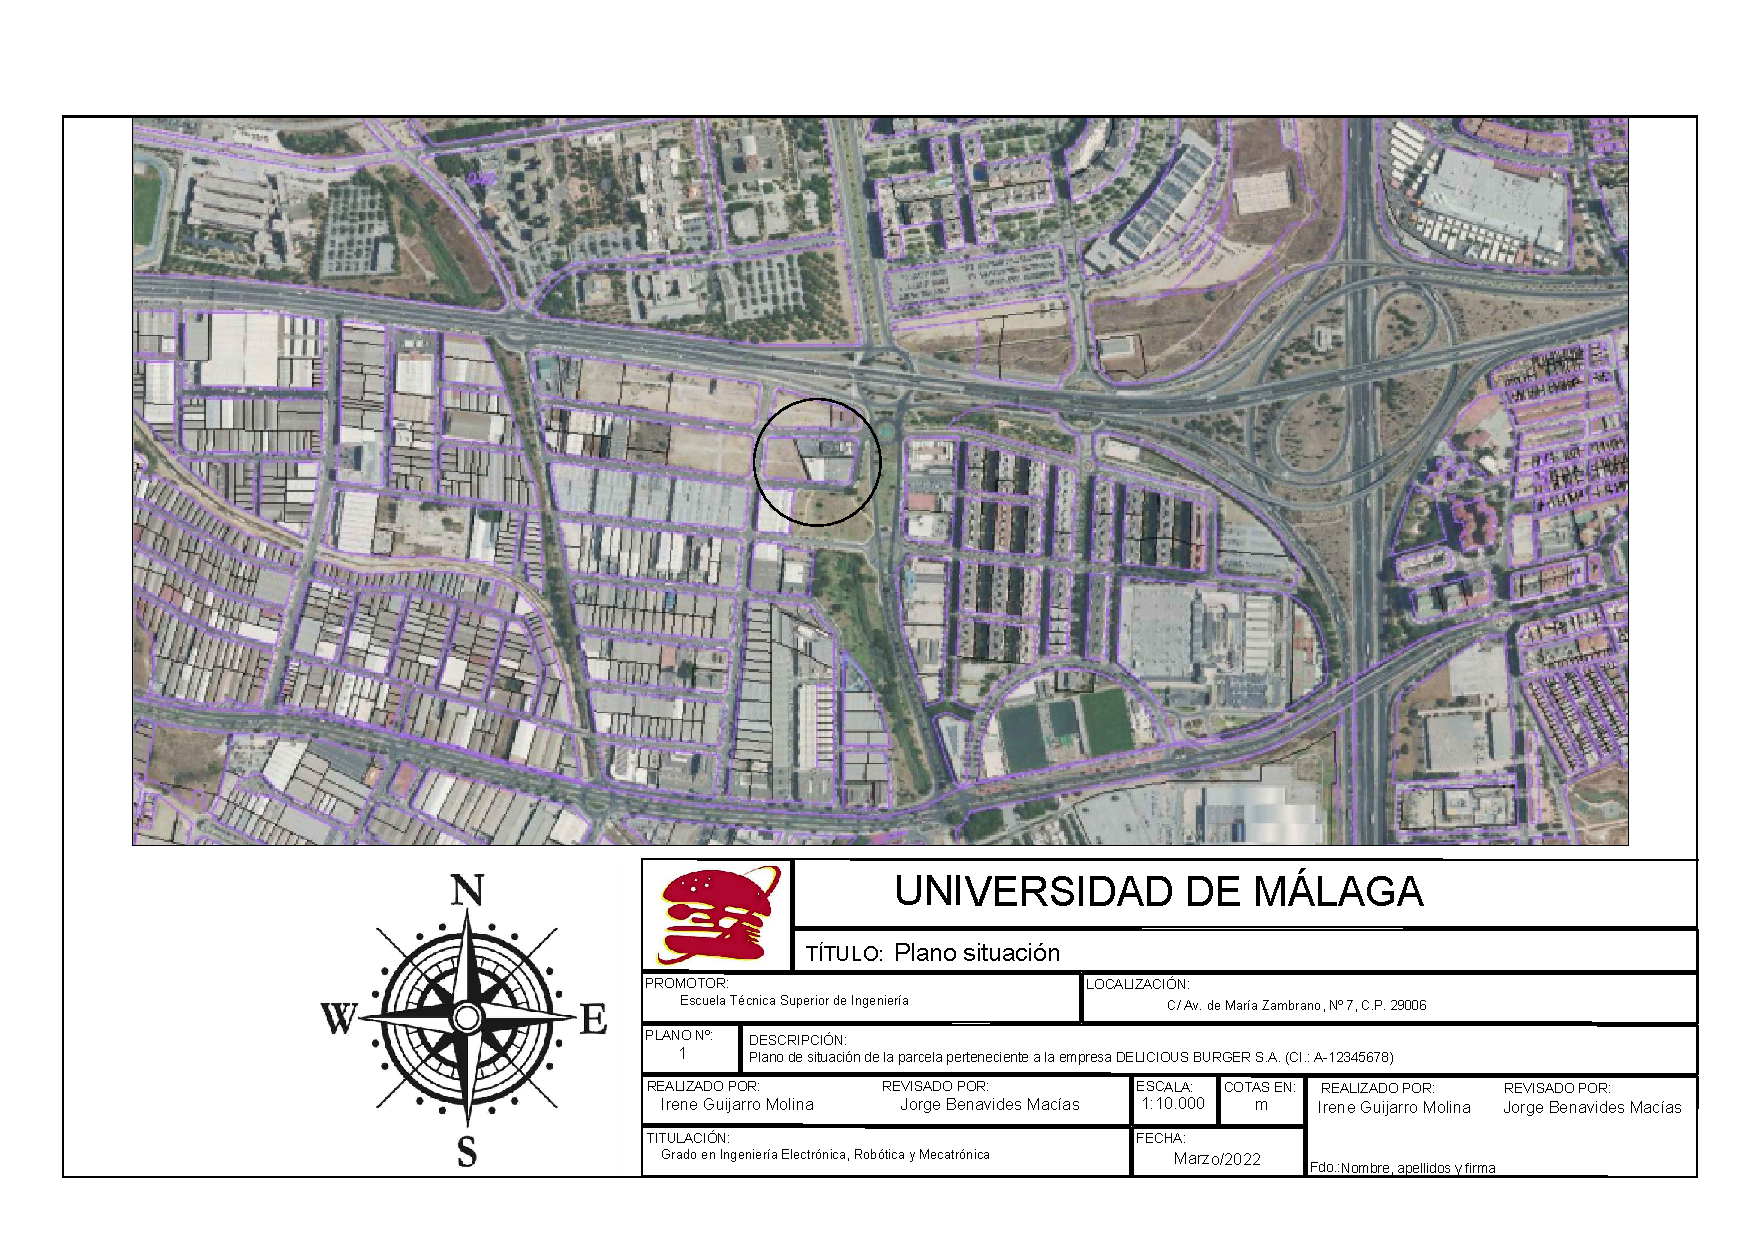
\includepdf[scale=1,angle=90,pages=-,addtotoc={1,subsection,1,Plano de situación,plano:situacion}]{archivos/Plano_situacion_DEF.pdf}

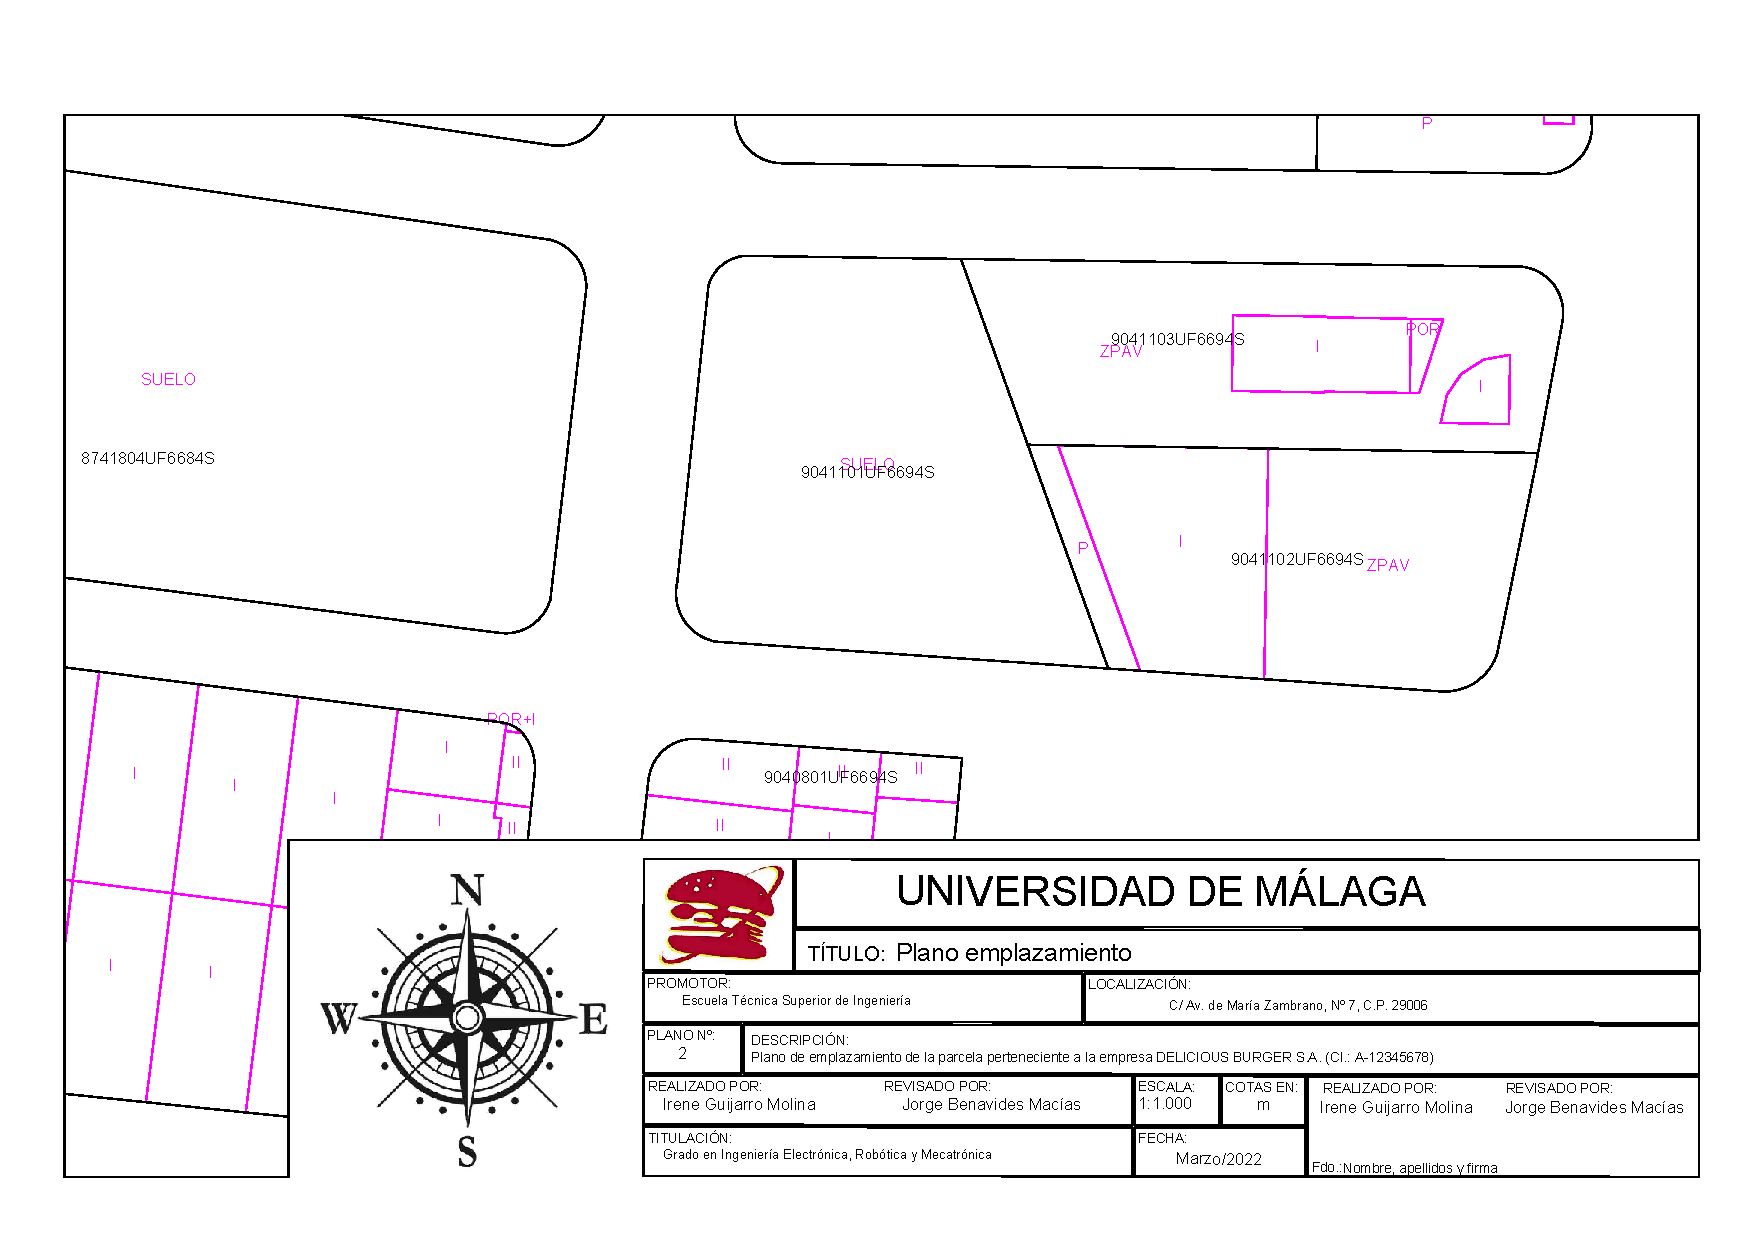
\includepdf[scale=1,angle=90,pages=-,addtotoc={1,subsection,1,Plano de emplazamiento,plano:emplazamiento}]{archivos/Plano_emplazamiento_DEF.pdf}

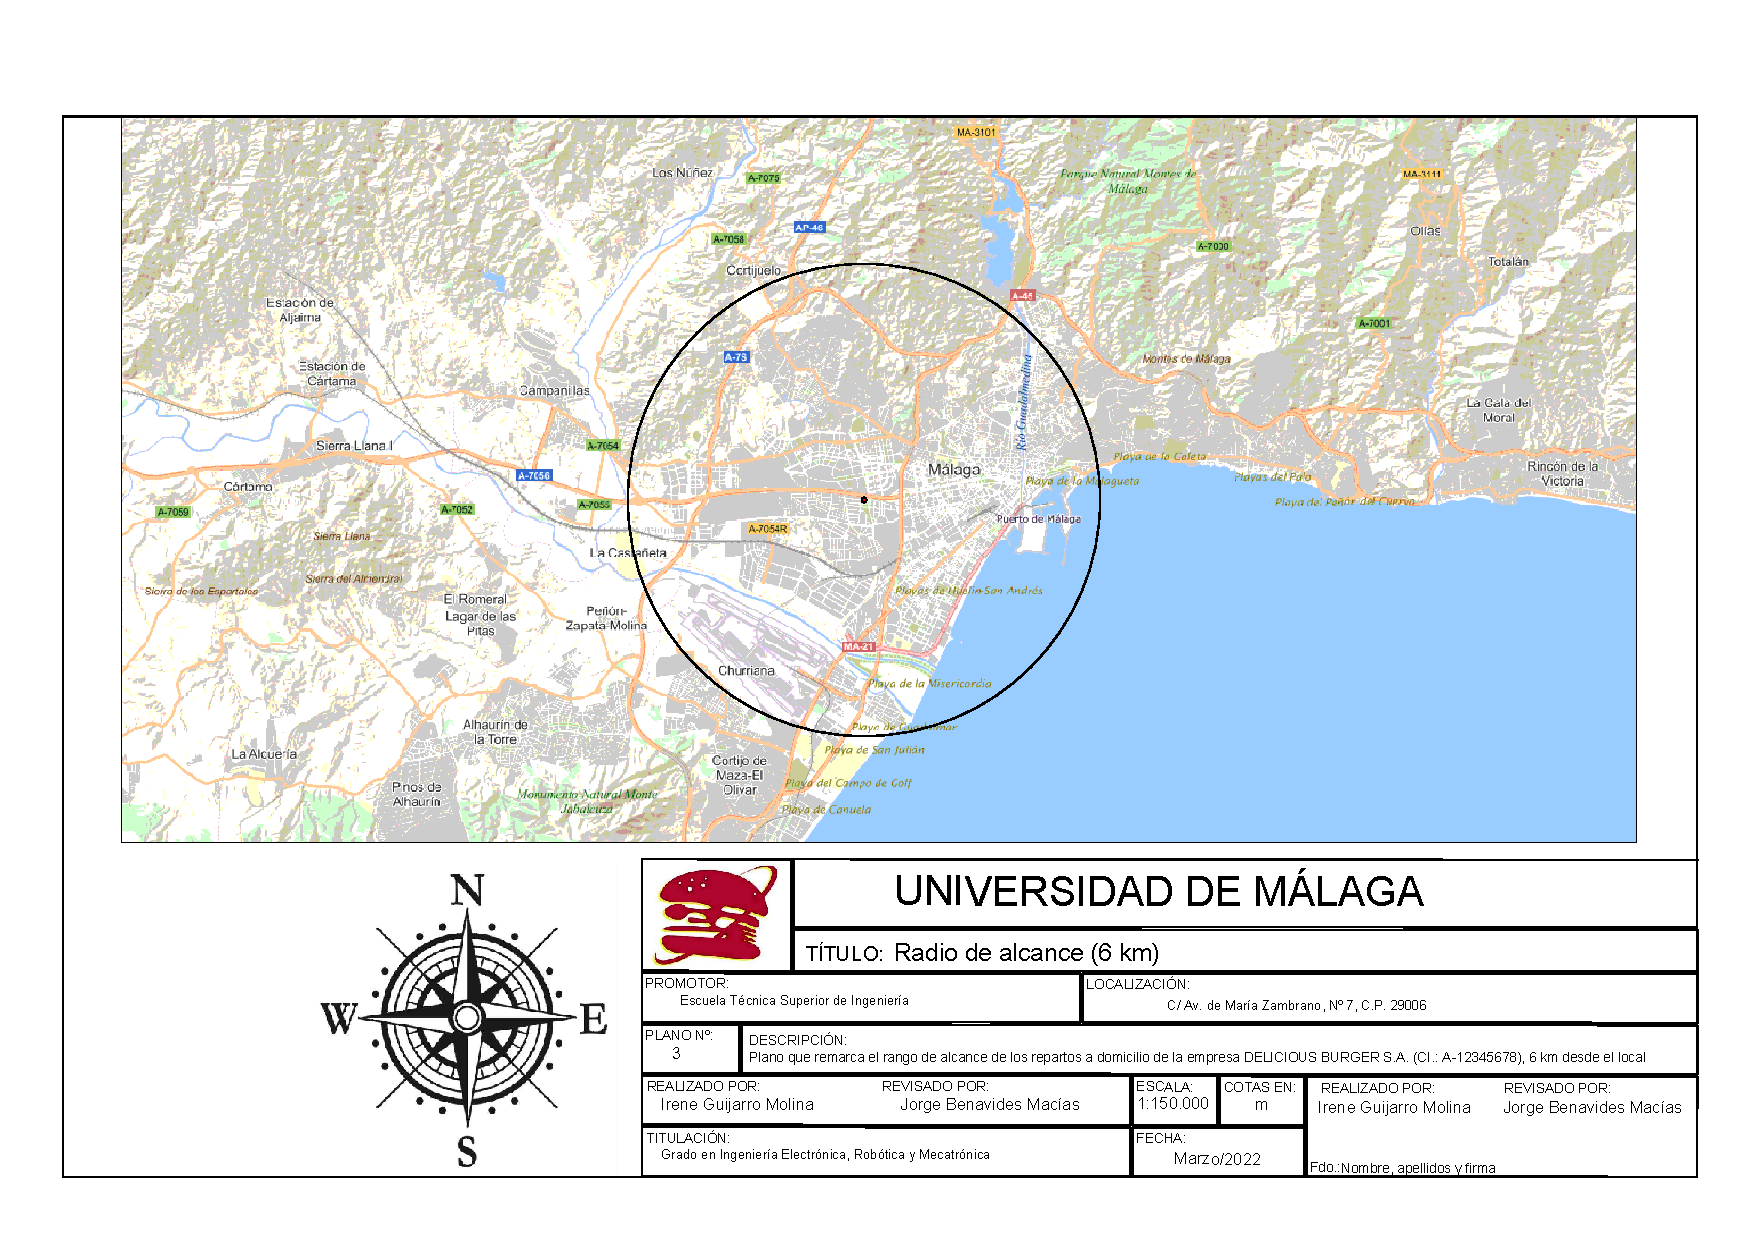
\includepdf[scale=1,angle=90,pages=-,addtotoc={1,subsection,1,Plano radio de alcance,plano:radio}]{archivos/Plano_radio_DEF.pdf}
\newpage
\section{Ciclomotor gasolina}
\label{anexo:Ciclomotor Gasolina}

Los \gls{ciclomotores} son vehículos que se han usado durante años para realizar el reparto a domicilio por su simplicidad, bajo coste y las prestaciones que ofrece para maniobras. Hoy en día, dado el desarrollo tecnológico y la reducción de costes en otros vehículos, el uso del ciclomotor ha disminuido, sin embargo, siguen siendo una referencia, en cuanto a reparto se refiere.

\begin{figure}[h]
    \centering
    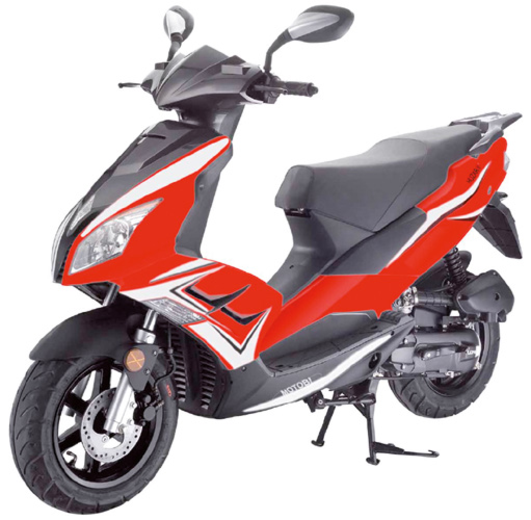
\includegraphics[scale = 1]{archivos/ciclomotor.pdf}
    \caption{Ciclomotor básico.}
    \label{fig:ciclomotor_basico}
\end{figure}

Al igual que otros vehículos, la \gls{dgt} recoge una serie de normas que deben cumplir todos los poseedores de un ciclomotor \cite{dgtciclomotores,boe11722}.

Las normas más destacables que influyen en la valoración de un modelo son las siguientes:
\begin{itemize}
    \item Está prohibido circular con el escape libre y emitir ruidos, gases u otros contaminantes.
    \item No podrán tener más luces y catadióptricos que los instalados por el fabricante.
    \item Los ciclomotores llevarán obligatoriamente un espejo retrovisor en el lado izquierdo. \textit{Opcionalmente, podrán llevar otro en el lado derecho.}
\end{itemize}

Acorde la normativa impuesta por la \gls{dgt} para matricular un ciclomotor, la tasa que corresponde es la 1.2 y asciende a 27,85 \glssymbol{euro}, esto quiere decir que al precio total de los ciclomotores hay que incluir el precio de la matriculación  \cite{dgtciclomotores}.


% El equipamiento que debe llevar el conductor de un ciclomotor es el siguiente:

% \begin{itemize}
%     \item Un casco, que debe estar homologado y correctamente abrochado. 
%     \item Chalecos u otros elementos reflectantes, ropas de color claro, casco con elementos reflectantes.
%     \item Sistema de alumbrado en perfectas condiciones con luces delanteras y traseras potentes, bien regladas y limpias.
% \end{itemize}



La \gls{itv} no contempla en su \textit{manual de modificaciones de vehículos} \cite{itvciclomotores} los cambios en la carrocería de los ciclomotores, por lo tanto, cualquier cambio de imagen para seguir la identidad corporativa de la empresa es de libre elección.

\subsection{Catálogo de modelos}
Después de una búsqueda exhaustiva de ciclomotores específicos para el reparto, se ha llegado a la conclusión de que los siguientes modelos satisfacen las necesidades expuestas anteriormente \cite{kymcofichatecnica, apriliafichatecnica, piaggiofichatecnica,peugeotfichatecnicars,peugeotfichatecnicaspeed,apriliasxr50,motormapfre}.
% kymcagility50
\begin{table}[h]
\resizebox{\textwidth}{!}{
\begin{tabular}{cccccccc}
\hline
\multicolumn{1}{|c|}{}                           & \multicolumn{1}{c|}{Precio {[}\gls{euro}{]}} & \multicolumn{1}{c|}{Homologación} & \multicolumn{1}{c|}{Cilindrada  {[}\gls{cc}{]}} & \multicolumn{1}{c|}{Consumo {[}\gls{litroporkilometro}{]}} & \multicolumn{1}{c|}{Depósito de gasolina {[}\gls{litros}{]}} & \multicolumn{1}{c|}{Emisiones \gls{dioxidodecarbono} {[}\gls{gramosporkilometros}{]}} & \multicolumn{1}{c|}{Peso {[}\gls{kg}{]}} \\ \hline
\multicolumn{1}{|c|}{KYMCO Agility Carry 50 E5}  & \multicolumn{1}{c|}{1.840,00}           & \multicolumn{1}{c|}{Euro 5}       & \multicolumn{1}{c|}{50}                   & \multicolumn{1}{c|}{2}                  & \multicolumn{1}{c|}{6}                            & \multicolumn{1}{c|}{47}                       & \multicolumn{1}{c|}{105}           \\ \hline
\multicolumn{1}{|c|}{Aprilia SXR 50}             & \multicolumn{1}{c|}{2.499,00}           & \multicolumn{1}{c|}{Euro 5}       & \multicolumn{1}{c|}{50}                   & \multicolumn{1}{c|}{2.5}                & \multicolumn{1}{c|}{7}                            & \multicolumn{1}{c|}{58}                       & \multicolumn{1}{c|}{100}           \\ \hline
\multicolumn{1}{|c|}{Liberty 50 Euro 5}          & \multicolumn{1}{c|}{2.499,00}           & \multicolumn{1}{c|}{Euro 3}       & \multicolumn{1}{c|}{49}                   & \multicolumn{1}{c|}{2.3}                & \multicolumn{1}{c|}{6}                            & \multicolumn{1}{c|}{48}                       & \multicolumn{1}{c|}{88}            \\ \hline
\multicolumn{1}{|c|}{Speedfight 50 4T EURO 5}    & \multicolumn{1}{c|}{2.990,00}           & \multicolumn{1}{c|}{L1e-B}        & \multicolumn{1}{c|}{50}                   & \multicolumn{1}{c|}{2.3}                & \multicolumn{1}{c|}{8}                            & \multicolumn{1}{c|}{51}                       & \multicolumn{1}{c|}{107}           \\ \hline
\multicolumn{1}{|c|}{Peugeot TWEET 50 RS EURO 5} & \multicolumn{1}{c|}{2.390,00}           & \multicolumn{1}{c|}{L1e-B}        & \multicolumn{1}{c|}{49}                   & \multicolumn{1}{c|}{2.4}                & \multicolumn{1}{c|}{5.4}                          & \multicolumn{1}{c|}{53}                       & \multicolumn{1}{c|}{100}           \\ \hline
                                                 &                                     &                                   &                                           &                                         &                                                   &                                               &                                   
\end{tabular}}
\caption{Comparación de distintos modelos de ciclomotores de reparto.}
\label{tab:comparacion de distintos modelos de ciclomotores de reparto}
\end{table}

La \autoref{tab:comparacion de distintos modelos de ciclomotores de reparto} recoge las principales características de diversas motos. Considerando la mejor relación calidad-precio, la mejor opción en cuanto al consumo, emisiones, depósito y peso, se ha llegado a la conclusión de que la moto más óptima para las condiciones que presenta la empresa es la \textbf{``KYMCO Agility Carry 50 E5''}.

La \textbf{``KYMCO Agility Carry 50 E5''}, es el modelo más barato de los cinco, se encuendra dentro de la categoría de vehículos L1, cuenta con una homologación \gls{euro5} \cite{euro5}, el mejor consumo respecto al resto, un depósito grande que permitirá recorrer largas distancias y las emisiones de \gls{dioxidodecarbono} son las más bajas, en contra parte el peso de la moto es elevado, pero que, comparado con otros modelos en el que la diferencia es de 2 \gls{kg} o 5 \gls{kg} y las prestaciones son menores, no tiene mucha importancia.

\newpage
% \addcontentsline{toc}{section}{Referencias}
% \section*{Referencias}
% \label{referencias_nucleo}
% \makeatletter
% \def\@bibitem#1{\item\if@filesw \immediate\write\@auxout
%   {\string\bibcite{#1}{A\the\value{\@listctr}}}\fi\ignorespaces}
% \def\@biblabel#1{[A{#1}]}
% \makeatother
% \printbibheading[title={Referencias},heading=bibintoc]
\nocite{*}
\newrefcontext[labelprefix=\thesection.]
\printbibheading[title={Referencias},heading=subbibintoc]
\printbibliography[heading=none,resetnumbers=true,keyword=ciclogasoref]
\newpage

\newpage
\section{Motocicleta gasolina}
\label{anexo_scooter_gasolina}
Las motocicletas son vehículos ligeros y ágiles utilizados para moverse con facilidad por la ciudad, por ello son utilizados por empresas de reparto, ya que aseguran una rápida entrega.

Se tiene que tener en consideración que las motocicletas, como cualquier otro vehículo, deben de pagar impuestos y tasas. Este coste será la suma de:

\begin{itemize}
    \item Impuesto de matriculación: las motocicletas de 125 \glssymbol{cc} tienen un impuesto de matriculación de 99,77 \glssymbol{euro}.
    \item Impuesto de circulación: para las motocicletas de 125 \glssymbol{cc}, el importe de dicho impuesto es de 8,55 \glssymbol{euro} anuales.
    
\end{itemize}

\subsection{Catálogo de modelos}

Se ha obtenido la \autoref{tabla: Comparación de distintos modelos de motocicletas de reparto.} de modelos y características de varias motocicletas de combustión mediante la investigación en páginas web de varios proveedores. Necesitamos una motocicleta que cumpla unos requisitos que nos faciliten la labor de reparto, por eso de entre las opciones se ha escogido el modelo “KYMCO AGILITY CARRY 125”, con un precio de mercado de 2.149,00 \glssymbol{euro}. Cumple que tenga gran autonomía y lo más importante, está especializada para las tareas de reparto.

\begin{table}[H]
\centering
\resizebox{\textwidth}{!}{
\begin{tabular}{|c|c|c|c|c|c|}
\hline
\textbf{Modelo}                   & \textbf{Autonomía (\gls{km})} & \textbf{Precio (\glssymbol{euro})} & \textbf{Capacidad(\glssymbol{litros})} & \textbf{Consumo(100 \glssymbol{litroporkilometro})} & \textbf{\glssymbol{euro}/\glssymbol{km}} \\ \hline
\textbf{Liberty 50 Euro 5}        & 240                     & 2.499,99       & 6                     & 2,5                       & 0,05          \\ \hline
\textbf{HONDA Vision 110}         & 245                     & 2.390,00       & 4,9                   & 2                         & 0,04          \\ \hline
\textbf{PEUGEOT Tweet 125 Active} & 190                     & 2.525,00      & 5,7                   & 3                         & 0,06          \\ \hline
\textbf{KYMCO Agility Carry 125}  & 250                     & 2.149,00       & 6,5                   & 2,6                       & 0,05          \\ \hline
\end{tabular}}
\caption{Comparación de distintos modelos de motocicletas de reparto.}
\label{tabla: Comparación de distintos modelos de motocicletas de reparto.}
\end{table}
\newpage
\section{Scooter eléctrico}
\label{anexo_scooter_electrico}
Los scooters eléctricos están empezando a ser muy usados, son una alternativa menos contaminante que su homólogo de gasolina y cuentan con planes de ayuda por parte del gobierno. Todo esto hace que sea una alternativa a considerar por muchas empresas para renovar su flota de reparto.

Estos vehículos eléctricos tienen un menor coste de mantenimiento que uno de gasolina, siendo el coste de tan solo 126 \glssymbol{euro} anuales. Esto es debido a que no necesitan cambio de aceite ni transmisión.

\subsection{Catálogo de modelos}

Se ha obtenido la \autoref{tabla: Comparación de distintos modelos de scooters de reparto.} de modelos y características de varias motocicletas de combustión mediante la investigación en páginas web de varios proveedores. Necesitamos una motocicleta que cumpla unos requisitos que nos faciliten la labor de reparto, por eso de entre las opciones se ha escogido el modelo “Askoll eS1”. Cumple que tenga gran autonomía y bajo tiempo de recarga. Aunque no cuente con el plan de ayudas MOVES III que supone un descuento de 1.100 \glssymbol{euro} en la compra sigue siendo más barata y con más autonomía que las que sí cuentan con él.

\begin{table}[H]
\centering
\resizebox{\textwidth}{!}{
\begin{tabular}{|c|c|c|c|c|}
\hline
\textbf{Modelo}                    & \textbf{Autonomía (\glssymbol{km})} & \textbf{Precio (\glssymbol{euro})} & \textbf{Capacidad(\glssymbol{kilovatiohora})} & \textbf{\glssymbol{euro}/\glssymbol{km}} \\ \hline
\textbf{Super Soco Cux}            & 80                      & 2.495,00       & 1,8                     & 0,000820      \\ \hline
\textbf{Askoll eS1}                & 100                     & 2.685,00       & 2,1                     & 0,00765       \\ \hline
\textbf{Askoll eS3 (MOVES III)}    & 96                      & 3.878,00       & 3,2                     & 0,01215       \\ \hline
\textbf{Linze Road L3 (MOVES III)} & 80                      & 3.490,00       & 2,88                    & 0,01312       \\ \hline
\end{tabular}}
\caption{Comparación de distintos modelos de scooters de reparto.}
\label{tabla: Comparación de distintos modelos de scooters de reparto.}
\end{table}

\newpage
\section{Patinete eléctrico}
\label{anexo_patienete eléctrico}

Los patinetes eléctricos son una alternativa como medio de transporte que ha ido ganando popularidad entre los ciudadanos dado su bajo coste frente a otros medios más convencionales y la libertad de movilidad que ofrece.

Actualmente, no existe una normativa que abarque a todas las comunidades autónomas de España, sin embargo, existe una normativa básica proporcionada por la \gls{dgt} \cite{dgtpatinete,recomendacionespatinete,instrucciondgt}, donde se recogen normas establecidas en algunas de las ciudades principales de España, como Barcelona, Madrid o Sevilla.

Basándonos en la normativa generalizada de la \gls{dgt} se deben cumplir las siguientes normas para poder circular con los patinetes eléctricos:
\begin{itemize}
    \item El conductor debe tener como mínimo 16 años de edad.
    \item El patinete debe estar provisto de luces frontales y traseras, tal y como lo llevan las motos, y deberán emplearse siguiendo las normas de circulación.
    \item No es obligatorio el uso de casco o chaleco reflectante, a menos que se utilice en carreteras, donde si será obligatorio el uso de chaleco reflectante.
    \item Dado el tipo de vehículo no es obligatorio poseer seguro, pero se recomienda tener uno en caso de accidentes \cite{noticiasegurospatinete,noticiasegurospatinete2}.
    \item Solo pueden circular por los carriles 30 designados, carriles bicis, o en su defecto por acera en caso de no existir alguna de las dos alternativas anteriores, siempre y cuando se reduzca la velocidad y se le dé preferencia a los peatones.
    \item La velocidad máxima por carretera es de 25 \glssymbol{km}/\glssymbol{hora}
    \item Solo pueden aparcarse en las zonas especiales \cite{aparcamientopatinete,aparcamientopatinetemapa} designadas para patinetes eléctricos (véase imagen/mapa o tabla), o en su defecto, zonas donde no molesten o se empleen mobiliario público.
\end{itemize}

Por otro lado, hay que tener en consideración las multas \cite{normativapatinete} que pueden recibir los conductores. Las cantidades pueden diferir, pero las posibles multas son:
\begin{itemize}
    \item Circular por aceras o zonas de peatones donde existe carril, bici o carretera - 200 \glssymbol{euro}
    \item Aparcar fuera de zona de estacionamiento: 200 \glssymbol{euro}
    \item Uso de teléfono o cascos de audio mientras se conduce: 200 \glssymbol{euro}
    \item Llevar dos pasajeros: 90 \glssymbol{euro}
    \item No llevar casco o chaleco en zonas obligatorias: 90 \glssymbol{euro}
    \item Exceder velocidad máxima: 200 \glssymbol{euro}
    \item Consumo de drogas, alcohol o conducción temerosa: 500-1000 \glssymbol{euro}
\end{itemize}

El conductor no está obligado a poseer carné de conducción de patinetes, pero debe tener bajo su poder, bien sea en documento físico o documento electrónico, el certificado \gls{ce} y ficha técnica del vehículo \cite{cetallerdelpatinete}, proporcionado por cada empresa vendedora de patinetes. En las \autoref{fig:CE patinete 1} y \autoref{fig:CE patinete 2} \cite{ceejemplo} se recogen como debe de ser un certificado \gls{ce}.

\begin{figure}[H]
    \centering
    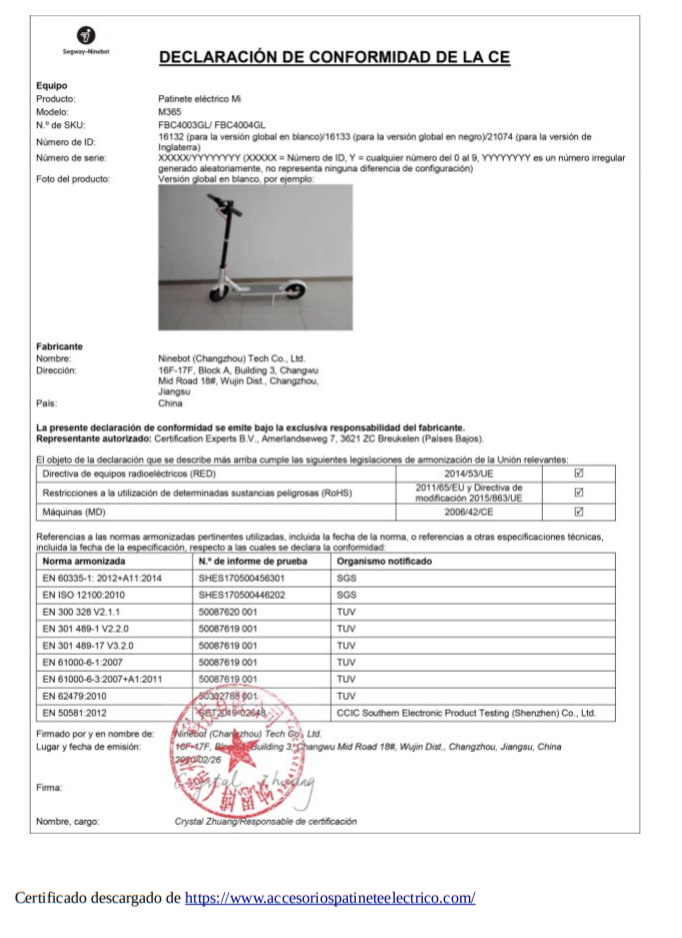
\includegraphics[scale=0.8]{archivos/CE patinete 1.png}
    \caption{\gls{ce} Patinete - Parte 1.}
    \label{fig:CE patinete 1}
\end{figure}

\begin{figure}[H]
    \centering
    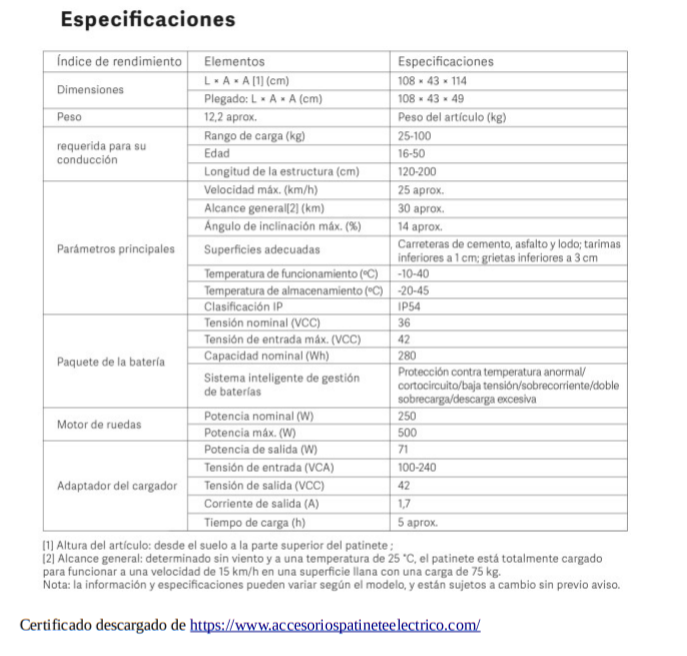
\includegraphics[scale=0.8]{archivos/CE patinete 2.png}
    \caption{\gls{ce} Patinete - Parte 2.}
    \label{fig:CE patinete 2}
\end{figure}

En la \autoref{tabla: modelo_patinete_electrico} se recogen algunos modelos de patinetes eléctricos existentes en el mercado actualmente, junto con algunas de sus características más destacables para el estudio.

\begin{table}[h]
\centering
\resizebox{1\textwidth}{!}{%
\begin{tabular}{|l|c|c|c|c|c|c|c|c|c|c|}
\hline
\multicolumn{1}{|c|}{\textbf{Modelo}} & \textbf{\begin{tabular}[c]{@{}c@{}}Autonomía\\ (\glssymbol{km})\end{tabular}} & \textbf{\begin{tabular}[c]{@{}c@{}}Vel. máx.\\ (\glssymbol{km}/\glssymbol{hora})\end{tabular}} & \textbf{\begin{tabular}[c]{@{}c@{}}Carga máx.\\ (\glssymbol{kg})\end{tabular}} & \textbf{\begin{tabular}[c]{@{}c@{}}Escalada máx\\ (\%)\end{tabular}} & \textbf{\begin{tabular}[c]{@{}c@{}}Absorción\\ choque\end{tabular}} & \textbf{\begin{tabular}[c]{@{}c@{}}Resistencia\\ al agua\end{tabular}} & \textbf{\begin{tabular}[c]{@{}c@{}}Potencia\\ (\glssymbol{vatios})\end{tabular}} & \textbf{\begin{tabular}[c]{@{}c@{}}Tiempo\\ carga (\glssymbol{hora})\end{tabular}} & \textbf{\begin{tabular}[c]{@{}c@{}}Capacidad\\ (\glssymbol{vatiohora})\end{tabular}} & \textbf{\begin{tabular}[c]{@{}c@{}}Precio\\ (\glssymbol{euro})\end{tabular}} \\ \hline
\textbf{\begin{tabular}[c]{@{}l@{}}Xiaomi Mi Electric \\ Scooter 3 Negro\end{tabular}} & 30 & 25 & 100 & 16 & Si & ?? & 600 & 5,5 & 275 & 427,47  \\ \hline
\textbf{\begin{tabular}[c]{@{}l@{}}Segway Ninebot KickScooter \\ F30E Patinete Eléctrico 10"\end{tabular}} & 30 & 25 & 120 & 15 & No & Si & 300 & 6,5 & 367 & 435,00  \\ \hline
\textbf{\begin{tabular}[c]{@{}l@{}}Segway Ninebot KickScooter \\ F40E Patinete Eléctrico 10"\end{tabular}} & 40 & 25 & 120 & 20 & No & Si & 350 & 6,5 & 367 & 504,99  \\ \hline
\textbf{\begin{tabular}[c]{@{}l@{}}Xiaomi Mi Electric Scooter \\ 1S Patinete Eléctrico Negro\end{tabular}} & 30 & 25 & 100 & 14 & Si & Si & 500 & 5,5 & 275 & 380,48  \\ \hline
\textbf{\begin{tabular}[c]{@{}l@{}}Infiniton CITYJam Pro \\ Patinete Eléctrico Negro\end{tabular}} & 40 & 25 & 100 & 15 & Si & Si & 350 & 6,5 & 350 & 376,62  \\ \hline
\end{tabular}%
}
\caption{Modelos de patinetes eléctricos.}
\label{tabla: modelo_patinete_electrico}

\end{table}

\newpage
% \addcontentsline{toc}{section}{Referencias}
% \section*{Referencias}
% \label{referencias_nucleo}
% \makeatletter
% \def\@bibitem#1{\item\if@filesw \immediate\write\@auxout
%   {\string\bibcite{#1}{A\the\value{\@listctr}}}\fi\ignorespaces}
% \def\@biblabel#1{[A{#1}]}
% \makeatother
% \printbibheading[title={Referencias},heading=bibintoc]
\nocite{*}
\newrefcontext[labelprefix=\thesection.]
\printbibheading[title={Referencias},heading=subbibintoc]
\printbibliography[heading=none,resetnumbers=true,keyword=patineteelec]
\newpage

\newpage
\section{Bicicletas eléctricas}
\label{bicicleta_electrica}

\subsection{Consideraciones previas}

Las bicicletas de pedaleo deben de llevar siempre pedales y no pueden funcionar con un acelerador, por lo que es totalmente ilegal conducir por la vía pública las ``mini-bicicleta" sin pedales, según recoge el BOE y la normativa de circulación. Según la normativa vigente, excluiremos del estudio este tipo de vehículo. 

Las bicicletas eléctricas propiamente hablando son reconocidas como ``ciclo de pedaleo asistido" según el BOE N.º 124 \cite{boe124}, lo que implica que aunque tienen motor eléctrico auxiliar, no pueden ser propulsadas exclusivamente haciendo uso del mismo, por lo que son vehículos híbridos entre eléctrico y manual.

\subsection{Modelo F.Lli Schiano E-Moon}

Actualmente, una de las mejores bicicletas eléctricas del mercado calidad-precio que cumple con todas las normativas vigentes es el modelo F.Lli Schiano E-Moon, que está a la venta por 729 \glssymbol{euro}. 

Respecto a sus características, posee un motor delantero ANANDA M129F de 250 \glssymbol{vatios} de potencia y 36 \glssymbol{voltios}, que permite alcanzar velocidades de hasta 25 \glssymbol{velocidad}. Presenta una batería de litio GREENWAY YJ145 36 \glssymbol{voltios} 13 \glssymbol{amperiohora} 468 \glssymbol{vatiohora}, con una vida útil de entre 4 y 6 años y una autonomía de hasta 120 \glssymbol{km} con 6 horas de carga completa. 

Su sistema de frenado es V-Brake en las ruedas delantera y trasera, ambos neumáticos son Kenda de 26 pulgadas. El cuerpo de la bicicleta no es plegable, es de una aleación de aluminio resistente, aunque no ligera (25 \glssymbol{kg}). Consta de una caja de cambios Shimano Tourney TY21 de 7 velocidades, un timbre, una luz delantera y otra trasera. 
Cumple todos los requisitos para ser considerada una bicicleta eléctrica:

\begin{itemize}
\item Tener dos ruedas, tal como considera El Real Decreto 2822/1998, de 23 de diciembre \cite{boe2822} que aprueba el Reglamento General de Vehículos.
\item Contar con un motor eléctrico cuya potencia máxima no exceda los 250 \glssymbol{vatios}.
\item Alcanzar una velocidad máxima asistida de 25 \glssymbol{velocidad}.
\item El motor ha de encender con el pedaleo y apagarse al llegar a 25 \glssymbol{velocidad} o cuando el pedaleo cese.
\end{itemize}

Al cumplir todos los requisitos anteriores no es necesario seguro obligatorio, matrícula, tarjeta de inspección técnica, casco ni permiso de conducción para circular por las vías públicas. No obstante, sí es necesario que el vehículo cuente con:


\begin{itemize}
\item Doble sistema de frenado, un freno para la rueda delantera y otro para la trasera.
\item Timbre. 
\item Luces de posición. La luz delantera debe ser de color blanco y la posterior de color rojo.
\item Señalización trasera.
\end{itemize}

Todas las especificaciones numeradas están incluidas en el modelo seleccionado.

Las bicicletas eléctricas no tienen restricciones relevantes de circulación en la vía pública, pueden usar los carriles bici o la carretera en su defecto. Además, si fuese necesario pueden circular por el arcén en autovías.

\subsection{Viabilidad del modelo}

Tal como se recoge en el \hyperref[plano:radio]{\hyperlink{plano:radio}{Plano 3}} del \refanexo{anexo_planos}, el rango de alcance de los repartos es de 6 \glssymbol{km} poniendo como centro la localización de la sede. Haciendo uso de los cálculos recogidos en la \autoref{tab:Calculo del número de bicicletas suponiendo distancia media por reparto 5 km}, siguiendo la misma metodología del \refanexo{anexo_calculos_sobre_vehiculos}, son necesarias unas 10 bicicletas eléctricas, las cuales se usarán durante todo el día y se recargarán generalmente por la noche, en el horario de cierre del negocio (24:00-9:00).

% Tabla x
\begin{table}[H]
\centering
\begin{tabular}{l|c|c|c|c|}
\cline{2-5}
 & \begin{tabular}[c]{@{}c@{}}TRAMO \\ HORARIO 1\end{tabular} & \begin{tabular}[c]{@{}c@{}}TRAMO \\ HORARIO 2\end{tabular} & \begin{tabular}[c]{@{}c@{}}TRAMO \\ HORARIO 3\end{tabular} & \begin{tabular}[c]{@{}c@{}}TRAMO \\ HORARIO 4\end{tabular} \\ \cline{2-5} 
 & \begin{tabular}[c]{@{}c@{}}Lunes-Jueves\\ (9:00-20:00)\end{tabular} & \begin{tabular}[c]{@{}c@{}}Lunes-Jueves\\ (20:00-0:00)\end{tabular} & \begin{tabular}[c]{@{}c@{}}Viernes-Domingo\\ (9:00-20:00)\end{tabular} & \begin{tabular}[c]{@{}c@{}}Viernes-Domingo\\ (20:00-1:00)\end{tabular} \\ \hline
\multicolumn{1}{|l|}{Nº pedidos} & 40 & 50 & 60 & 120 \\ \hline
\multicolumn{1}{|l|}{\begin{tabular}[c]{@{}l@{}}Distancia total \\ a recorrer (km)\end{tabular}} & 200 & 250 & 300 & 600 \\ \hline
\multicolumn{1}{|l|}{\begin{tabular}[c]{@{}l@{}}Tiempo total de \\ reparto (min)\end{tabular}} & 660 & 240 & 660 & 300 \\ \hline
\multicolumn{1}{|l|}{\begin{tabular}[c]{@{}l@{}}Tiempo estimado por \\ pedido (min/pedido)\end{tabular}} & 20 & 20 & 20 & 20 \\ \hline
\multicolumn{1}{|l|}{\begin{tabular}[c]{@{}l@{}}Nº pedidos realizables \\ por vehículo\end{tabular}} & 33 & 12 & 33 & 15 \\ \hline
\multicolumn{1}{|l|}{\begin{tabular}[c]{@{}l@{}}Nº vehículos \\ simultáneos necesarios\end{tabular}} & 2 & 5 & 2 & 8 \\ \hline
\multicolumn{1}{|l|}{\begin{tabular}[c]{@{}l@{}}Nº de turnos \\ de vehículos\end{tabular}} & 1 & 1 & 2 & 1 \\ \hline
\multicolumn{1}{|l|}{\begin{tabular}[c]{@{}l@{}}Nº vehículos \\ totales necesarios\end{tabular}} & 2 & 5 & 4 & 8 \\ \hline
\end{tabular}
\caption{Cálculo del número de bicicletas suponiendo distancia media por reparto 5 \glssymbol{km}.}
\label{tab:Calculo del número de bicicletas suponiendo distancia media por reparto 5 km}
\end{table}


Suponiendo una revisión mensual de mantenimiento \cite{feuvertes}, el precio de la luz \cite{precio_luz_bici} en el horario en el que se producirá la recarga de los vehículos y el coste de adquisición de los vehículos \cite{precio_bici} quedan que están recogidos en la \autoref{tab:Costes economicos necesarios para el calculo del presupuesto}, el coste de adquisición de los vehículos junto y el resto de servicios requeridos por los mismos supondría 9.000,00 \glssymbol{euro} el primer año, tal como se expresa en la \autoref{eqn:presupuesto anual bicicletas}. En los años siguientes, el presupuesto para vehículos sería de aproximadamente 1.000,00 \glssymbol{euro}.


\begin{equation}
\label{eqn:presupuesto anual bicicletas}
220,06+10*(676+44,25+90)+8*114,76=9\.240,64\text{ \glssymbol{euro}}
\end{equation}


De este modo, se estima que en 10 años la empresa habrá invertido 1.800,00 \glssymbol{euro} de media anuales en los vehículos, incluido mantenimiento, reparaciones y recargas.


\begin{table}[H]
\centering
\begin{tabular}{|l|c|}
\hline
Precio medio de la luz 24:00-7:00 (€/kWh) & 0,2645 \\ \hline
Capacidad batería vehículo (\glssymbol{kilovatiohora}) & 0,25 \\ \hline
Presupuesto anual en recargas (\glssymbol{euro}) & 220,06 \\ \hline
Precio unitario/vehículo (\glssymbol{euro}) & 676,00 \\ \hline
Precio unitario equipamiento (\glssymbol{euro}) & 114,76 \\ \hline
Precio unitario mantenimiento bicicleta eléctrica en Feuvert (€/año) & 44,25 \\ \hline
Reserva económica unitaria para sustituciones (€/año) & 90,00 \\ \hline
\end{tabular}
\caption{Costes económicos necesarios para el cálculo del presupuesto.}
\label{tab:Costes economicos necesarios para el calculo del presupuesto}
\end{table}

En vista de los resultados económicos y de buena imagen de la empresa hacia el consumidor debido al método de reparto ecológico, es evidente que es una buena opción a tener en cuenta entre los distintos vehículos del mercado. No obstante, ha de considerarse que para ciertos trayectos próximos a los 6 km o que impliquen el uso de algún tramo de autovía, no es aconsejable el uso de este modelo eléctrico por seguridad del transportista y/o por exceso del tiempo de reparto deseado. 

Asimismo, las opciones de estacionamiento de bicicletas son limitadas, semáforos, farolas y barandillas no están permitidas, por lo que se ha de localizar un aparcamiento de bicicletas o estacionarlas del mismo modo que una moto convencional (en este último método, sería necesario también el uso de una cadena especial).

\newpage
% \addcontentsline{toc}{section}{Referencias}
% \section*{Referencias}
% \label{referencias_nucleo}
% \makeatletter
% \def\@bibitem#1{\item\if@filesw \immediate\write\@auxout
%   {\string\bibcite{#1}{A\the\value{\@listctr}}}\fi\ignorespaces}
% \def\@biblabel#1{[A{#1}]}
% \makeatother
% \printbibheading[title={Referencias},heading=bibintoc]
\nocite{*}
\newrefcontext[labelprefix=\thesection.]
\printbibheading[title={Referencias},heading=subbibintoc]
\printbibliography[heading=none,resetnumbers=true,keyword=bicielec]
\newpage

\newpage
\section{Cálculos sobre vehículos}
\label{anexo_calculos_sobre_vehiculos}

Este anexo contiene todos los cálculos necesarios para realizar el análisis completo de los distintos vehículos viables, para todos ellos se ha procedido al estudio de dos casos distintos.

El primero de ellos, hace referencia al supuesto en el que se realizan  pedidos de forma individualizada, con un trayecto medio de 5 \glssymbol{km} y un tiempo de reparto de 5 minutos. El segundo caso, alude al supuesto en el que se realicen dos pedidos por reparto, con un trayecto medio de 7,5 \glssymbol{km} y se empleen 10 minutos en el reparto. Esta información queda plasmada en la tabla \autoref{tabla:tabla_datos_comunes}, en la cual también se recogen otros datos pertinentes comunes a los diversos cálculos contenidos en el anexo.


\begin{table}[H]
\centering
\begin{tabular}{|l|c|}
\hline

%Impuestos en motocicletas
%Seguro en motocicletas
%Seguro en patinetes
%Mantenimiento motocicletas eléctricas
%Mantenimiento 
%Equipamiento para motocicletas
%Equipamiento para patinetes
Precio medio de la   luz (\glssymbol{euro}/\glssymbol{kilovatiohora}) & 0,11193 \\ \hline
Precio medio de la gasolina (\glssymbol{euro}/\glssymbol{litros}) & 1,38 \\ \hline
Distancia a recorrer por reparto (\glssymbol{km}) & 5 \\ \hline
Distancia a recorrer por reparto doble (\glssymbol{km}) & 7,5 \\ \hline
Tiempo por reparto (\glssymbol{minuto}) & 5 \\ \hline
Tiempo por reparto doble (\glssymbol{minuto}) & 10 \\ \hline
Precio equipamiento patinetes (\glssymbol{euro}) & 114,76 \\ \hline
Precio equipamiento motocicletas/ciclomotores (\glssymbol{euro}) & 190,58 \\ \hline
Seguro en patinetes (\glssymbol{euro}) & 35 \\ \hline
Seguro en motocicletas/ciclomotores (\glssymbol{euro}) & 265 \\ \hline
Impuesto circulación patinetes (\glssymbol{euro}) & 0 \\ \hline
Impuesto circulación motocicletas/ciclomotores (\glssymbol{euro}) & 8,55 \\ \hline
Impuesto matriculación patinetes (\glssymbol{euro}) & 0 \\ \hline
\end{tabular}
%Impuesto matriculación motocicletas/ciclomotores (\glssymbol{euro}) & 0 \\ \hline
% Impuesto circulación motocicletas de 125 \glssymbol{cc} (\glssymbol{euro}) & 99,77 \\ \hline
\caption{Datos comunes para los distintos vehículos viables.}
\label{tabla:tabla_datos_comunes}
\end{table}


Además de los dos escenarios distintos, se valorarán cuatro franjas horarias de reparto y los dos intervalos semanales que se plantean como datos de estudio. El primer escenario que se estudia abarca de lunes a jueves, con primer turno de trabajo de nueve de la mañana a ocho de la tarde, y segundo turno de 8 de la tarde a doce de la noche, recogidos en la \autoref{tab:distribucion de reparto}. La empresa demandante nos proporciona como información un reparto homogéneo en el tiempo y por cada intervalo correspondiente. Se observa que el volumen de repartos es mayor los fines de semana que en el resto, por lo que se espera obtener en los resultados una mayor cantidad de vehículos en esos tramos.

Otro limitante a tener en cuenta es la autonomía del vehículo, por lo que se calcula el tiempo que se encuentra circulando en carretera con ayuda de la velocidad estimada y la distancia de recorrido. Una vez obtenido el tiempo en carretera, se le incluyen el tiempo de reparto, donde el repartidor se desplaza de la calle a la vivienda, entrega el pedido, cobra el importe y regresa al vehículo.

Con el tiempo estimado por pedido y el tiempo total de la franja horaria se determina el número de pedidos que podría realizar una persona sin tener en cuenta las limitaciones de la autonomía. Según el valor que se obtenga, se compara con el número de pedidos que son necesario cumplir, y se añaden tantos vehículos como sean necesarios hasta igualar o superar la cifra de pedidos.

A partir de toda la información anterior, se puede calcular el tiempo que tardará el vehículo en necesitar una recarga de combustible o batería, permitiendo así obtener el número de vehículos extraordinarios en caso de estar trabajando con los modelos eléctricos.

Así pues, conociendo la cantidad de vehículos en total, se podrá estimar la cantidad de vehículos que debe adquirir la empresa para cumplir con la demanda de cada una de las franjas de este estudio.

Por otro lado, se debe tener en cuenta en los cálculos el tiempo de repostaje o recarga del vehículo. En el caso de vehículos a gasolina no tendrá un valor considerable, ya que el tiempo de llenado de depósito no supera los pocos minutos. Por el contrario, en los vehículos eléctricos, en el supuesto que la empresa opte por recargas de baterías del vehículo, se tendrá en consideración el tiempo donde no puede ser empleado para los repartos.

\subsection{Ciclomotor gasolina 50cc, KYMCO Agility Carry 50 E5}
\label{Ciclomotor gasolina 50cc, KYMCO Agility Carry 50}
%% kilómetro que recorre la moto
%% litros que puede llevar
%% precio de la moto
Entre los distintos ciclomotores del mercado, el modelo KYMCO Agility Carry 50 E5 resulta ser uno de los más ventajosos. A continuación, en la \autoref{tab:Datos ciclomotores de gasolina} se indican las características necesarias para realizar un análisis económico del vehículo.

\begin{table}[H]
\centering
\begin{tabular}{|l|c|}
\hline
Alcance máximo con   carga completa    & 350-300 \glssymbol{km} \\ \hline
Alcance estimado con carga completa    & 300 \glssymbol{km}    \\ \hline
Velocidad máxima alcanzable            & 60 \glssymbol{km}/\glssymbol{hora}  \\ \hline
Velocidad media estimada               & 40 \glssymbol{km}/\glssymbol{hora}  \\ \hline
\end{tabular}
\caption{Datos ciclomotores de gasolina.}
\label{tab:Datos ciclomotores de gasolina}
\end{table}

A efectos prácticos, la \autoref{tab:Análisis detallado motocicletas de gasolina, viajes de 5 km} coincide con la \autoref{tab:Análisis detallado ciclomotores de gasolina, viajes de 5 km} y la \autoref{tab:Análisis detallado motocicletas de gasolina, viajes de 7,5 km} es idéntica a la \autoref{tab:Análisis detallado ciclomotores de gasolina, viajes de 7,5 km}, debido a que con números relativamente pequeños, las características diferentes entre los modelos KYMCO Agility Carry 50 E5 y KYMCO Agility Carry 125 apenas interfieren en el estudio de la entrega de pedidos. 

\begin{table}[H]
\centering
\begin{tabular}{l|c|c|c|c|}
\cline{2-5}
 & \begin{tabular}[c]{@{}c@{}}TRAMO \\ HORARIO 1\end{tabular} & \begin{tabular}[c]{@{}c@{}}TRAMO \\ HORARIO 2\end{tabular} & \begin{tabular}[c]{@{}c@{}}TRAMO \\ HORARIO 3\end{tabular} & \begin{tabular}[c]{@{}c@{}}TRAMO \\ HORARIO 4\end{tabular} \\ \cline{2-5} 
 & \begin{tabular}[c]{@{}c@{}}Lunes-Jueves \\ (9:00-20:00)\end{tabular} & \begin{tabular}[c]{@{}c@{}}Lunes-Jueves \\ (20:00-0:00)\end{tabular} & \begin{tabular}[c]{@{}c@{}}Viernes-Domingo \\ 9:00-20:00)\end{tabular} & \begin{tabular}[c]{@{}c@{}}Viernes-Domingo \\ 20:00-1:00)\end{tabular} \\ \hline
\multicolumn{1}{|l|}{Nº pedidos} & 40 & 50 & 60 & 120 \\ \hline
\multicolumn{1}{|l|}{\begin{tabular}[c]{@{}l@{}}Distancia total \\ a recorrer (\glssymbol{km})\end{tabular}} & 200 & 250 & 300 & 600 \\ \hline
\multicolumn{1}{|l|}{\begin{tabular}[c]{@{}l@{}}Tiempo total de \\ reparto (\glssymbol{minuto})\end{tabular}} & 660 & 240 & 660 & 300 \\ \hline
\multicolumn{1}{|l|}{\begin{tabular}[c]{@{}l@{}}Tiempo estimado por \\ pedido (\glssymbol{minuto}/pedido)\end{tabular}} & 12,5 & 12,5 & 12,5 & 12,5 \\ \hline
\multicolumn{1}{|l|}{\begin{tabular}[c]{@{}l@{}}Nº pedidos realizables \\ por vehículo\end{tabular}} & 52,8 & 19,2 & 52,8 & 24 \\ \hline
\multicolumn{1}{|l|}{\begin{tabular}[c]{@{}l@{}}Nº vehículos \\ simultáneos necesarios\end{tabular}} & 1 & 3 & 2 & 5 \\ \hline
\multicolumn{1}{|l|}{\begin{tabular}[c]{@{}l@{}}Nº de turnos \\ de vehículos\end{tabular}} & 1 & 1 & 1 & 1 \\ \hline
\multicolumn{1}{|l|}{\begin{tabular}[c]{@{}l@{}}Nº vehículos \\ totales necesarios\end{tabular}} & 1 & 3 & 2 & 5 \\ \hline
\end{tabular}
\caption{Análisis detallado ciclomotores de gasolina, viajes de 5 km.}
\label{tab:Análisis detallado ciclomotores de gasolina, viajes de 5 km}
\end{table}



\begin{table}[H]
\centering
\begin{tabular}{l|c|c|c|c|}
\cline{2-5}
 & \begin{tabular}[c]{@{}c@{}}TRAMO \\ HORARIO 1\end{tabular} & \begin{tabular}[c]{@{}c@{}}TRAMO \\ HORARIO 2\end{tabular} & \begin{tabular}[c]{@{}c@{}}TRAMO \\ HORARIO 3\end{tabular} & \begin{tabular}[c]{@{}c@{}}TRAMO \\ HORARIO 4\end{tabular} \\ \cline{2-5} 
 & \begin{tabular}[c]{@{}c@{}}Lunes-Jueves \\ (9:00-20:00)\end{tabular} & \begin{tabular}[c]{@{}c@{}}Lunes-Jueves \\ (20:00-0:00)\end{tabular} & \begin{tabular}[c]{@{}c@{}}Viernes-Domingo \\ 9:00-20:00)\end{tabular} & \begin{tabular}[c]{@{}c@{}}Viernes-Domingo \\ 20:00-1:00)\end{tabular} \\ \hline
\multicolumn{1}{|l|}{Nº pedidos} & 20 & 25 & 30 & 60 \\ \hline
\multicolumn{1}{|l|}{\begin{tabular}[c]{@{}l@{}}Distancia total \\ a recorrer (\glssymbol{km})\end{tabular}} & 150 & 187,5 & 225 & 450 \\ \hline
\multicolumn{1}{|l|}{\begin{tabular}[c]{@{}l@{}}Tiempo total de \\ reparto (\glssymbol{minuto})\end{tabular}} & 660 & 240 & 660 & 300 \\ \hline
\multicolumn{1}{|l|}{\begin{tabular}[c]{@{}l@{}}Tiempo estimado por \\ pedido (\glssymbol{minuto}/pedido)\end{tabular}} & 21,25 & 21,25 & 21,25 & 21,25 \\ \hline
\multicolumn{1}{|l|}{\begin{tabular}[c]{@{}l@{}}Nº pedidos realizables \\ por vehículo\end{tabular}} & 31 & 11 & 31 & 14 \\ \hline
\multicolumn{1}{|l|}{\begin{tabular}[c]{@{}l@{}}Nº vehículos \\ simultáneos necesarios\end{tabular}} & 1 & 3 & 1 & 5 \\ \hline
\multicolumn{1}{|l|}{\begin{tabular}[c]{@{}l@{}}Nº de turnos \\ de vehículos\end{tabular}} & 1 & 1 & 1 & 1 \\ \hline
\multicolumn{1}{|l|}{\begin{tabular}[c]{@{}l@{}}Nº vehículos \\ totales necesarios\end{tabular}} & 1 & 3 & 1 & 5 \\ \hline
\end{tabular}
\caption{Análisis detallado ciclomotores de gasolina, viajes de 7,5 km.}
\label{tab:Análisis detallado ciclomotores de gasolina, viajes de 7,5 km}
\end{table}

Los vehículos de gasolina no deben ser sustituidos pues su repostaje apenas supone tiempo y no se ha considerado en este estudio. Según la  \autoref{tab:Análisis detallado motocicletas de gasolina, viajes de 5 km} y la \autoref{tab:Análisis detallado motocicletas de gasolina, viajes de 7,5 km}, se deduce que son necesarios 5 vehículos para el tramo horario más desfavorable (cuello de botella) para las dos opciones contempladas.


Por último, a partir del número de vehículos necesarios, los datos de la \autoref{tab:Datos ciclomotores de gasolina}, los de la \autoref{tabla:tabla_datos_comunes} y otros datos de cálculo incluidos en la misma \autoref{tab:Presupuesto motillo Peter}, se ha elaborado un presupuesto de este modelo, tanto en un primer año como un a lo largo de 10 años.

\begin{table}[H]
\centering
\begin{tabular}{|l|c|}
\hline
N.º repostajes semanales caso 1 & 6 \\ \hline
N.º repostajes semanales caso 2 & 5 \\ \hline
Capacidad depósito del vehículo (\glssymbol{litros}) & 6 \\ \hline
Coste recarga unitario (\glssymbol{euro}) & 8,28 \\ \hline
Gasto semanal en  repostajes caso 1 (\glssymbol{euro}) & 41,40 \\ \hline
Gasto semanal en  repostajes caso 2 (\glssymbol{euro}) & 33,12 \\ \hline
Presupuesto anual en repostajes caso 1 (\glssymbol{euro}) & 2.152,80 \\ \hline
Presupuesto anual en repostajes caso 2 (\glssymbol{euro}) & 1.722,24 \\ \hline
Precio unitario/vehículo (\glssymbol{euro}) & 1.999 \\ \hline
Precio unitario mantenimiento (\glssymbol{euro}) & 239 \\ \hline
Reserva de sustitución por vehículo (\glssymbol{euro}) & 50 \\ \hline
Presupuesto para   vehículos primer año caso 1 (\glssymbol{euro}) & 16.052,70 \\ \hline
Presupuesto para vehículos primer año   caso 2 (\glssymbol{euro}) & 15.622,14 \\ \hline
Presupuesto para vehículos anual  caso 1 (\glssymbol{euro}) & 4.965,55 \\ \hline
Presupuesto para vehículos anual caso 2 (\glssymbol{euro}) & 4.534,99 \\ \hline
Presupuesto en vehículos a 10 años, caso 1 (\glssymbol{euro}) & 60.742,65 \\ \hline
Presupuesto en vehículos a 10 años, caso 2 (\glssymbol{euro}) & 56.437,05 \\ \hline
\end{tabular}
\caption{Presupuesto ciclomotor KYMCO Agility Carry 50 E5.}
\label{tab:Presupuesto motillo Peter}
\end{table}

\subsection{Motocicleta gasolina 125cc, KYMCO Agility Carry 125}
\label{sub_anexo_calculos_motocicleta}
En esta sección del anexo, se recogen los datos numéricos relativos a la motocicleta de gasolina KYMCO Agility Carry 125. Tomando como referencia datos de la
\autoref{tabla:tabla_datos_comunes}, se añaden especificaciones concretas del modelo en la tabla \autoref{tab:Datos motocileta de gasolina}.


\begin{table}[H]
\centering
\begin{tabular}{|l|c|}
\hline
Alcance máximo con   carga completa    & 250-300 \glssymbol{km} \\ \hline
Alcance estimado con carga completa    & 250 \glssymbol{km}    \\ \hline
Velocidad máxima alcanzable            & 120 \glssymbol{km}/\glssymbol{hora}  \\ \hline
Velocidad media estimada               & 40 \glssymbol{km}/\glssymbol{hora}  \\ \hline
\end{tabular}
\caption{Datos motocicleta de gasolina.}
\label{tab:Datos motocileta de gasolina}
\end{table}


Los dos casos a analizar están reflejados en la \autoref{tab:Análisis detallado motocicletas de gasolina, viajes de 5 km} y la \autoref{tab:Análisis detallado motocicletas de gasolina, viajes de 7,5 km}. Para el estudio de este tipo de vehículo, no es necesario realizar ninguna gráfica adicional a las tablas obtenidas, pues al ser un vehículo de gasolina, repostar implica un par de minutos y no es necesario ningún cambio de vehículo.


\begin{table}[H]
\centering
\begin{tabular}{l|c|c|c|c|}
\cline{2-5}
 & \begin{tabular}[c]{@{}c@{}}TRAMO \\ HORARIO 1\end{tabular} & \begin{tabular}[c]{@{}c@{}}TRAMO \\ HORARIO 2\end{tabular} & \begin{tabular}[c]{@{}c@{}}TRAMO \\ HORARIO 3\end{tabular} & \begin{tabular}[c]{@{}c@{}}TRAMO \\ HORARIO 4\end{tabular} \\ \cline{2-5} 
 & \begin{tabular}[c]{@{}c@{}}Lunes-Jueves \\ (9:00-20:00)\end{tabular} & \begin{tabular}[c]{@{}c@{}}Lunes-Jueves \\ (20:00-0:00)\end{tabular} & \begin{tabular}[c]{@{}c@{}}Viernes-Domingo \\ 9:00-20:00)\end{tabular} & \begin{tabular}[c]{@{}c@{}}Viernes-Domingo \\ 20:00-1:00)\end{tabular} \\ \hline
\multicolumn{1}{|l|}{Nº pedidos} & 40 & 50 & 60 & 120 \\ \hline
\multicolumn{1}{|l|}{\begin{tabular}[c]{@{}l@{}}Distancia total \\ a recorrer (\glssymbol{km})\end{tabular}} & 200 & 250 & 300 & 600 \\ \hline
\multicolumn{1}{|l|}{\begin{tabular}[c]{@{}l@{}}Tiempo total de \\ reparto (\glssymbol{minuto})\end{tabular}} & 660 & 240 & 660 & 300 \\ \hline
\multicolumn{1}{|l|}{\begin{tabular}[c]{@{}l@{}}Tiempo estimado por \\ pedido (\glssymbol{minuto}/pedido)\end{tabular}} & 12,5 & 12,5 & 12,5 & 12,5 \\ \hline
\multicolumn{1}{|l|}{\begin{tabular}[c]{@{}l@{}}Nº pedidos realizables \\ por vehículo\end{tabular}} & 52,8 & 19,2 & 52,8 & 24 \\ \hline
\multicolumn{1}{|l|}{\begin{tabular}[c]{@{}l@{}}Nº vehículos \\ simultáneos necesarios\end{tabular}} & 1 & 3 & 2 & 5 \\ \hline
\multicolumn{1}{|l|}{\begin{tabular}[c]{@{}l@{}}Nº de turnos \\ de vehículos\end{tabular}} & 1 & 1 & 1 & 1 \\ \hline
\multicolumn{1}{|l|}{\begin{tabular}[c]{@{}l@{}}Nº vehículos \\ totales necesarios\end{tabular}} & 1 & 3 & 2 & 5 \\ \hline
\end{tabular}
\caption{Análisis detallado motocicletas de gasolina, viajes de 5 km.}
\label{tab:Análisis detallado motocicletas de gasolina, viajes de 5 km}
\end{table}



\begin{table}[H]
\centering
\begin{tabular}{l|c|c|c|c|}
\cline{2-5}
 & \begin{tabular}[c]{@{}c@{}}TRAMO \\ HORARIO 1\end{tabular} & \begin{tabular}[c]{@{}c@{}}TRAMO \\ HORARIO 2\end{tabular} & \begin{tabular}[c]{@{}c@{}}TRAMO \\ HORARIO 3\end{tabular} & \begin{tabular}[c]{@{}c@{}}TRAMO \\ HORARIO 4\end{tabular} \\ \cline{2-5} 
 & \begin{tabular}[c]{@{}c@{}}Lunes-Jueves \\ (9:00-20:00)\end{tabular} & \begin{tabular}[c]{@{}c@{}}Lunes-Jueves \\ (20:00-0:00)\end{tabular} & \begin{tabular}[c]{@{}c@{}}Viernes-Domingo \\ 9:00-20:00)\end{tabular} & \begin{tabular}[c]{@{}c@{}}Viernes-Domingo \\ 20:00-1:00)\end{tabular} \\ \hline
\multicolumn{1}{|l|}{Nº pedidos} & 20 & 25 & 30 & 60 \\ \hline
\multicolumn{1}{|l|}{\begin{tabular}[c]{@{}l@{}}Distancia total \\ a recorrer (\glssymbol{km})\end{tabular}} & 150 & 187,5 & 225 & 450 \\ \hline
\multicolumn{1}{|l|}{\begin{tabular}[c]{@{}l@{}}Tiempo total de \\ reparto (\glssymbol{minuto})\end{tabular}} & 660 & 240 & 660 & 300 \\ \hline
\multicolumn{1}{|l|}{\begin{tabular}[c]{@{}l@{}}Tiempo estimado por \\ pedido (\glssymbol{minuto}/pedido)\end{tabular}} & 21,25 & 21,25 & 21,25 & 21,25 \\ \hline
\multicolumn{1}{|l|}{\begin{tabular}[c]{@{}l@{}}Nº pedidos realizables \\ por vehículo\end{tabular}} & 31 & 11 & 31 & 14 \\ \hline
\multicolumn{1}{|l|}{\begin{tabular}[c]{@{}l@{}}Nº vehículos \\ simultáneos necesarios\end{tabular}} & 1 & 3 & 1 & 5 \\ \hline
\multicolumn{1}{|l|}{\begin{tabular}[c]{@{}l@{}}Nº de turnos \\ de vehículos\end{tabular}} & 1 & 1 & 1 & 1 \\ \hline
\multicolumn{1}{|l|}{\begin{tabular}[c]{@{}l@{}}Nº vehículos \\ totales necesarios\end{tabular}} & 1 & 3 & 1 & 5 \\ \hline
\end{tabular}
\caption{Análisis detallado motocicletas de gasolina, viajes de 7,5 km.}
\label{tab:Análisis detallado motocicletas de gasolina, viajes de 7,5 km}
\end{table}

En resumen, de este modelo serían necesarios cinco vehículos para realizar satisfactoriamente todos los pedidos deseados en ambos casos estudiados.
En cuanto al presupuesto, queda recogido en la \autoref{tab:Presupuesto motocicletas de gasolina}.

\begin{table}[H]
\centering
\begin{tabular}{|l|c|}
\hline
N.º repostajes semanales caso 1 & 6 \\ \hline
N.º repostajes semanales caso 2 & 5 \\ \hline
Capacidad depósito del vehículo (\glssymbol{litros}) & 6,5 \\ \hline
Coste recarga unitario (\glssymbol{euro}) & 8,28 \\ \hline
Gasto semanal en  repostajes caso 1 (\glssymbol{euro}) & 53,82 \\ \hline
Gasto semanal en  repostajes caso 2 (\glssymbol{euro}) & 44,85 \\ \hline
Presupuesto anual en repostajes caso 1 (\glssymbol{euro}) & 2.798,64 \\ \hline
Presupuesto anual en repostajes caso 2 (\glssymbol{euro}) & 2.332,20 \\ \hline
Precio unitario/vehículo (\glssymbol{euro}) & 2.149 \\ \hline
Precio unitario mantenimiento (\glssymbol{euro}) & 239 \\ \hline
Reserva de sustitución por vehículo (\glssymbol{euro}) & 100 \\ \hline
Presupuesto para   vehículos primer año caso 1 (\glssymbol{euro}) & 18.058,14 \\ \hline
Presupuesto para vehículos primer año   caso 2 (\glssymbol{euro}) & 17.591,70 \\ \hline
Presupuesto para vehículos anual  caso 1 (\glssymbol{euro}) & 5.861,39 \\ \hline
Presupuesto para vehículos anual caso 2 (\glssymbol{euro}) & 5.394,95 \\ \hline
Presupuesto en vehículos a 10 años, caso 1 (\glssymbol{euro}) & 70.810,65 \\ \hline
Presupuesto en vehículos a 10 años, caso 2 (\glssymbol{euro}) & 66.146,25 \\ \hline
\end{tabular}
\caption{Presupuesto motocicletas de gasolina.}
\label{tab:Presupuesto motocicletas de gasolina}
\end{table}

%x9" y las expresiones "z3" y "z4", se ha calculado que a lo largo de 10 años sería necesario invertir un total de 60.000 \glssymbol{euro}, unos 6.000 \glssymbol{euro} anuales aproximadamente. 

% Tabla x9

%\begin{equation}
%  16489,81+5234,81*9=63.603,1 \text{ \glssymbol{euro}} 
%\end{equation}

%\begin{equation}
%  16.043,65+4.788,65*9=59.141,5 \text{ \glssymbol{euro}}
%\end{equation}


\subsection{Motocicleta eléctrica, Askoll eS1}
\label{sub_anexo_calculos_motocicleta_eléctrica}
A continuación, se han recopilado los datos numéricos referentes a la motocicleta eléctrica Askoll eS1. Usando la de la tabla \autoref{tabla:tabla_datos_comunes} y los datos específicos del modelo de la \autoref{tabla: Datos_concretos_moto_electrica}, se han determinado el mínimo número de vehículos de este modelo necesarios para las dos hipótesis propuestas y los cuatro tramos horarios asignados.
%\textwidth
\begin{table}[H]
\centering
%\resizebox{}{!}{
\begin{tabular}{|l|c|}
\hline
Alcance máximo con   carga completa    & 100-120 \glssymbol{km} \\ \hline
Alcance estimado con carga completa    & 100 \glssymbol{km}    \\ \hline
Velocidad máxima alcanzable            & 45 \glssymbol{velocidad}  \\ \hline
Velocidad media estimada               & 40 \glssymbol{velocidad}  \\ \hline
Duración recarga            & 6 \glssymbol{hora} \\ \hline
\end{tabular}
\caption{Datos motocicleta eléctrica.}
\label{tabla: Datos_concretos_moto_electrica}
\end{table}


% Tabla x11
\begin{table}[H]
\centering
\resizebox{\textwidth}{!}{
\begin{tabular}{l|c|c|c|c|}
\cline{2-5}
 & \begin{tabular}[c]{@{}c@{}}TRAMO \\ HORARIO 1\end{tabular} & \begin{tabular}[c]{@{}c@{}}TRAMO \\ HORARIO 2\end{tabular} & \begin{tabular}[c]{@{}c@{}}TRAMO \\ HORARIO 3\end{tabular} & \begin{tabular}[c]{@{}c@{}}TRAMO \\ HORARIO 4\end{tabular} \\ \cline{2-5} 
 & \begin{tabular}[c]{@{}c@{}}Lunes-Jueves \\ (9:00-20:00)\end{tabular} & \begin{tabular}[c]{@{}c@{}}Lunes-Jueves \\ (20:00-0:00)\end{tabular} & \begin{tabular}[c]{@{}c@{}}Lunes-Jueves \\ 9:00-20:00)\end{tabular} & \begin{tabular}[c]{@{}c@{}}Viernes-Domingo \\ 20:00-1:00)\end{tabular} \\ \hline
\multicolumn{1}{|l|}{N.º pedidos} & 40 & 50 & 60 & 120 \\ \hline
\multicolumn{1}{|l|}{\begin{tabular}[c]{@{}l@{}}Distancia total \\ a recorrer (\glssymbol{km})\end{tabular}} & 200 & 250 & 300 & 600 \\ \hline
\multicolumn{1}{|l|}{\begin{tabular}[c]{@{}l@{}}Tiempo total de \\ reparto (\glssymbol{minuto})\end{tabular}} & 660 & 240 & 660 & 300 \\ \hline
\multicolumn{1}{|l|}{\begin{tabular}[c]{@{}l@{}}Tiempo estimado por \\ pedido (\glssymbol{minuto}/pedido)\end{tabular}} & 12,5 & 12,5 & 12,5 & 12,5 \\ \hline
\multicolumn{1}{|l|}{\begin{tabular}[c]{@{}l@{}}Nº pedidos realizables \\ por vehículo\end{tabular}} & 52,8 & 19,2 & 52,8 & 24,0 \\ \hline
\multicolumn{1}{|l|}{\begin{tabular}[c]{@{}l@{}}Nº vehículos \\ simultáneos necesarios\end{tabular}} & 1 & 3 & 2 & 5 \\ \hline
\multicolumn{1}{|l|}{\begin{tabular}[c]{@{}l@{}}Nº de turnos \\ de vehículos\end{tabular}} & 2 & 1 & 2 & 2 \\ \hline
\multicolumn{1}{|l|}{\begin{tabular}[c]{@{}l@{}}Nº vehículos \\ totales necesarios\end{tabular}} & 2 & 3 & 4 & 6 \\ \hline
\end{tabular}}
\caption{Estudio de pedidos para motocicletas eléctricas en viajes de 5 km.}
\label{tab:Estudio de pedidos para motocicletas eléctricas en viajes de 5 km}
\end{table}


\begin{table}[H]
\centering
\resizebox{\textwidth}{!}{
\begin{tabular}{l|c|c|c|c|}
\cline{2-5}
 & \begin{tabular}[c]{@{}c@{}}TRAMO \\ HORARIO 1\end{tabular} & \begin{tabular}[c]{@{}c@{}}TRAMO \\ HORARIO 2\end{tabular} & \begin{tabular}[c]{@{}c@{}}TRAMO \\ HORARIO 3\end{tabular} & \begin{tabular}[c]{@{}c@{}}TRAMO \\ HORARIO 4\end{tabular} \\ \cline{2-5} 
 & \begin{tabular}[c]{@{}c@{}}Lunes-Jueves \\ (9:00-20:00)\end{tabular} & \begin{tabular}[c]{@{}c@{}}Lunes-Jueves \\ (20:00-0:00)\end{tabular} & \begin{tabular}[c]{@{}c@{}}Viernes-Domingo \\ 9:00-20:00)\end{tabular} & \begin{tabular}[c]{@{}c@{}}Viernes-Domingo \\ 20:00-1:00)\end{tabular} \\ \hline
\multicolumn{1}{|l|}{Nº pedidos} & 20 & 25 & 30 & 60 \\ \hline
\multicolumn{1}{|l|}{\begin{tabular}[c]{@{}l@{}}Distancia total \\ a recorrer (\glssymbol{km})\end{tabular}} & 150 & 187,5 & 225 & 450 \\ \hline
\multicolumn{1}{|l|}{\begin{tabular}[c]{@{}l@{}}Tiempo total de \\ reparto (\glssymbol{minuto})\end{tabular}} & 660 & 240 & 660 & 300 \\ \hline
\multicolumn{1}{|l|}{\begin{tabular}[c]{@{}l@{}}Tiempo estimado por \\ pedido (\glssymbol{minuto}/pedido)\end{tabular}} & 21,3 & 21,3 & 21,3 & 21,3 \\ \hline
\multicolumn{1}{|l|}{\begin{tabular}[c]{@{}l@{}}Nº pedidos realizables \\ por vehículo\end{tabular}} & 31 & 11 & 31 & 14 \\ \hline
\multicolumn{1}{|l|}{\begin{tabular}[c]{@{}l@{}}Nº vehículos \\ simultáneos necesarios\end{tabular}} & 1 & 3 & 1 & 5 \\ \hline
\multicolumn{1}{|l|}{\begin{tabular}[c]{@{}l@{}}Nº de turnos \\ de vehículos\end{tabular}} & 2 & 1 & 3 & 1 \\ \hline
\multicolumn{1}{|l|}{\begin{tabular}[c]{@{}l@{}}Nº vehículos \\ totales necesarios\end{tabular}} & 2 & 3 & 3 & 5 \\ \hline
\end{tabular}}
\caption{Estudio de pedidos para motocicletas eléctricas en viajes de 7,5 km.}
\label{tab:Estudio de pedidos para motocicletas eléctricas en viajes de 7,5 km}
\end{table}


En función de los resultados recopilados en la \autoref{tab:Estudio de pedidos para motocicletas eléctricas en viajes de 5 km} y en la \autoref{tab:Estudio de pedidos para motocicletas eléctricas en viajes de 7,5 km}, son necesarias 10 motocicletas eléctricas para realizar el reparto de forma correcta en una de las hipótesis supuestas,8 para la segunda. Sin embargo, al tener en cuenta el tiempo que tarda este el modelo Askoll eS1 en cargarse completamente, el número de vehículos se puede reducir en ambas opciones, tal como se refleja en la \autoref{fig:motos_electricas_caso1} y en la \autoref{fig:motos_electricas_caso22}.

\begin{figure}[ht]
    \centering
    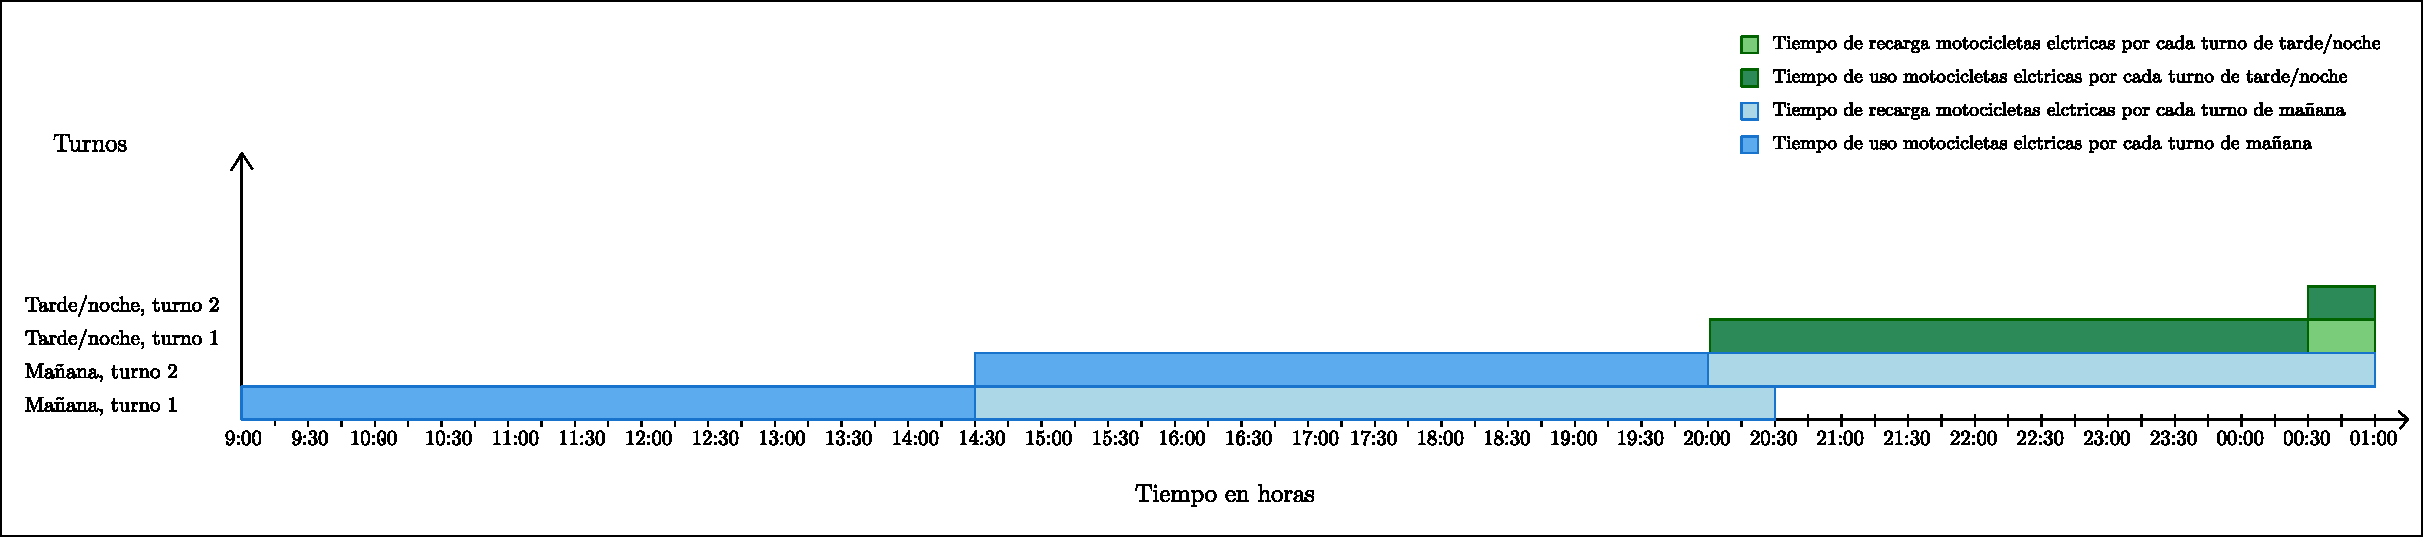
\includegraphics[width= \textwidth, height=12em]{archivos/caso1_motos_electricas.pdf}
    \caption{Representación turnos de motocicletas eléctricas en viajes de 5 \glssymbol{km}.}
    \label{fig:motos_electricas_caso1}
\end{figure}

La \autoref{fig:motos_electricas_caso1} muestra que durante el horario de mañana en el caso 1, tienen lugar 2 turnos de 2 vehículos cada uno (zona azul del gráfico). El color verde resalta el inicio del horario de tarde; en el primer turno se han de emplear 5 vehículos, mientras que en el segundo turno solo se emplea una motocicleta, la cual proviene del primer turno de la mañana.

\begin{figure}[ht]
    \centering
    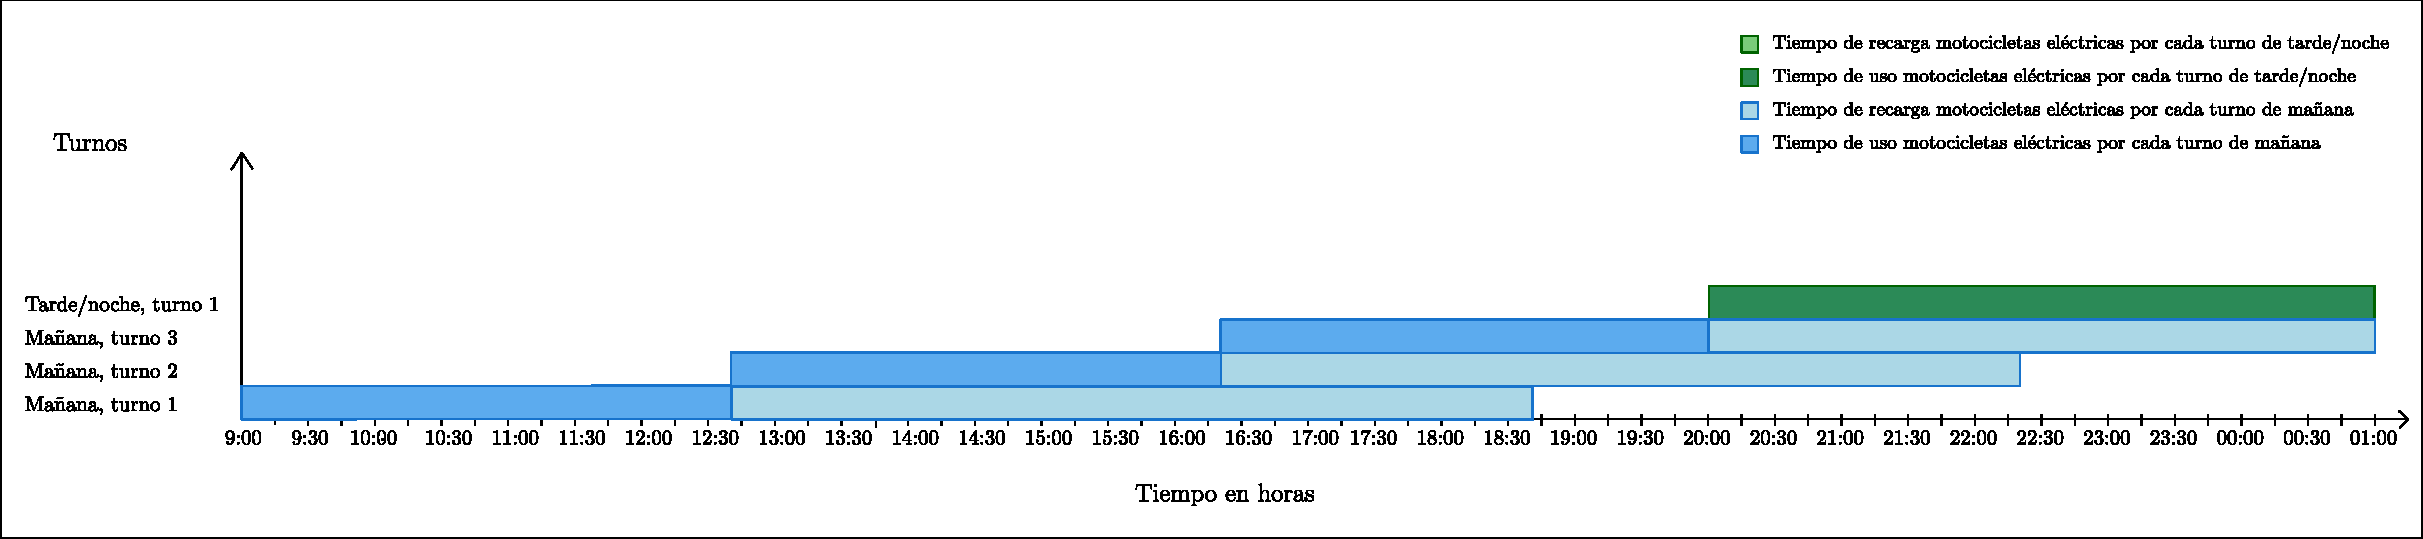
\includegraphics[width= \textwidth, height=12em]{archivos/caso2_motos_electricas.pdf}
    \caption{Representación turnos de motocicletas eléctricas en viajes de 7,5 \glssymbol{km}.}
    \label{fig:motos_electricas_caso22}
\end{figure}

Respecto a la \label{fig:motos_electricas_caso2}, que recoge la segunda hipótesis de repartos, se observan 4 turnos en total, 3 de mañana de 1 vehículo cada uno y 1 turno por la tarde de 5 vehículos simultáneos. En el turno de la tarde, como se debe reutilizar uno de los vehículos de la mañana solo son necesarios 7 vehículos en total. Es decir, se necesitan 9 motocicletas para el primer caso y 7 para el segundo caso de repartos.

Seguidamente, se agrupan los distintos gastos en la \autoref{tab:Estudio presupuestos modelo Askoll eS1}.

\begin{table}[H]
\centering
\begin{tabular}{|l|c|}
\hline
N.º recargas semanales caso 1 & 50 \\ \hline
N.º recargas semanales caso 2 & 44 \\ \hline
Capacidad batería vehículo (\glssymbol{kilovatiohora}) & 2,1 \\ \hline
Coste recarga unitario (\glssymbol{euro}) & 0,24 \\ \hline
Gasto semanal en  recargas caso 1 (\glssymbol{euro}) & 11,75 \\ \hline
Gasto semanal en  recargas caso 2 (\glssymbol{euro}) & 10,34 \\ \hline
Presupuesto anual en recargas caso 1 (\glssymbol{euro}) & 611,14 \\ \hline
Presupuesto anual en recargas caso 2 (\glssymbol{euro}) & 537,80 \\ \hline
Precio unitario/vehículo (\glssymbol{euro}) & 2.685 \\ \hline
Precio unitario mantenimiento (\glssymbol{euro}) & 126 \\ \hline
Reserva de sustitución por vehículo (\glssymbol{euro}) & 100 \\ \hline
Presupuesto para   vehículos primer año caso 1 (\glssymbol{euro}) & 30.475,64 \\ \hline
Presupuesto para vehículos primer año   caso 2 (\glssymbol{euro}) & 23.977,50 \\ \hline
Presupuesto para vehículos anual  caso 1 (\glssymbol{euro}) & 5.107,09 \\ \hline
Presupuesto para vehículos anual caso 2 (\glssymbol{euro}) & 4.034,65 \\ \hline
Presupuesto en vehículos a 10 años, caso 1 (\glssymbol{euro}) & 76.439,43 \\ \hline
Presupuesto en vehículos a 10 años, caso 2 (\glssymbol{euro}) & 60.289,36 \\ \hline
\end{tabular}
\caption{Estudio presupuestos modelo Askoll eS1.}
\label{tab:Estudio presupuestos modelo Askoll eS1}
\end {table}

%Empleando la tabla "x13" y las expresiones "z5" y "z6", se ha valorado que a lo largo de 10 años es necesario invertir un total de 40.000 \glssymbol{euro}, unos 4.000 \glssymbol{euro} anuales aproximadamente. 


%Análisis presupuestos modelo eSkoll

%\begin{equation}
%  15486,42+2898,52*9=41.573,1 \text{ \glssymbol{euro}}   
%\end{equation}
%\begin{equation}
%  15245,85+2657,95*9=39.167,4 \text{ \glssymbol{euro}}
%\end{equation}


\subsection{Infiniton CITYJam Pro}
\label{sub_anexo_calculos_patinete}

En la tabla \autoref{tabla: Datos_concretos_patinete} se han recogido las características específicas del modelo Infiniton CITYJam Pro con las que se van a trabajar para los cálculos correspondientes.


\begin{table}[H]
\centering
\begin{tabular}{|l|c|}
\hline
Alcance máximo con   carga completa    & 40-45 \glssymbol{km} \\ \hline
Alcance estimado con carga completa    & 40 \glssymbol{km}    \\ \hline
Velocidad máxima alcanzable            & 25 \glssymbol{velocidad}  \\ \hline
Velocidad media estimada               & 20 \glssymbol{velocidad}  \\ \hline
Duración recarga            & 6 \glssymbol{hora} 30 \glssymbol{minuto}  \\ \hline
\end{tabular}
\caption{Datos patinete eléctrico.}
\label{tabla: Datos_concretos_patinete}
\end{table}

Tal como se precisó anteriormente, se han supuesto dos hipótesis distintas a la hora de estudiar la distribución de los pedidos, lo que corresponde con la \autoref{tabla: analisis_detallado_patinete_5km} y la \autoref{tabla: analisis_detallado_patinete_7.5km}, respectivamente. En ellas, conocida la distancia total a recorrer por los vehículos, la duración de cada tramo horario considerado y los datos de la \autoref{tabla: Datos_concretos_patinete}, se ha obtenido el número de vehículos necesarios por cada uno de esos tramos.

% Tabla x3
\begin{table}[H]
\centering
\resizebox{\textwidth}{!}{
\begin{tabular}{l|c|c|c|c|}
\cline{2-5}
 & \begin{tabular}[c]{@{}c@{}}TRAMO \\ HORARIO 1\end{tabular} & \begin{tabular}[c]{@{}c@{}}TRAMO \\ HORARIO 2\end{tabular} & \begin{tabular}[c]{@{}c@{}}TRAMO \\ HORARIO 3\end{tabular} & \begin{tabular}[c]{@{}c@{}}TRAMO \\ HORARIO 4\end{tabular} \\ \cline{2-5} 
 & \begin{tabular}[c]{@{}c@{}}Lunes-Jueves \\ (9:00-20:00)\end{tabular} & \begin{tabular}[c]{@{}c@{}}Lunes-Jueves \\ (20:00-0:00)\end{tabular} & \begin{tabular}[c]{@{}c@{}}Viernes-Domingo \\ (9:00-20:00)\end{tabular} & \begin{tabular}[c]{@{}c@{}}Viernes-Domingo \\ (20:00-1:00)\end{tabular} \\ \hline
\multicolumn{1}{|l|}{Nº pedidos} & 40 & 50 & 60 & 120 \\ \hline
\multicolumn{1}{|l|}{\begin{tabular}[c]{@{}l@{}}Distancia total a \\ recorrer \glssymbol{km}\end{tabular}} & 200 & 250 & 300 & 600 \\ \hline
\multicolumn{1}{|l|}{\begin{tabular}[c]{@{}l@{}}Tiempo total de \\ reparto \glssymbol{minuto} \end{tabular}} & 660 & 240 & 660 & 300 \\ \hline
\multicolumn{1}{|l|}{\begin{tabular}[c]{@{}l@{}}Tiempo estimado \\ por pedido (\glssymbol{minuto}/pedido)\end{tabular}} & 20 & 20 & 20 & 20 \\ \hline
\multicolumn{1}{|l|}{\begin{tabular}[c]{@{}l@{}}Nº pedidos realizables \\ por vehículo\end{tabular}} & 33 & 12 & 33 & 15 \\ \hline
\multicolumn{1}{|l|}{\begin{tabular}[c]{@{}l@{}}Nº vehículos simultáneos \\ necesarios\end{tabular}} & 2 & 5 & 2 & 8 \\ \hline
\multicolumn{1}{|l|}{Nº de turnos de vehículos} & 3 & 2 & 4 & 2 \\ \hline
\multicolumn{1}{|l|}{\begin{tabular}[c]{@{}l@{}}Nº vehículos totales \\ necesarios\end{tabular}} & 6 & 10 & 8 & 16 \\ \hline
\end{tabular}}
\caption{Análisis detallado del reparto en patinete con viajes de 5 \glssymbol{km}.}
\label{tabla: analisis_detallado_patinete_5km}
\end{table}



\begin{table}[H]
\centering
\resizebox{\textwidth}{!}{
\begin{tabular}{l|c|c|c|c|}
\cline{2-5}
 & \begin{tabular}[c]{@{}c@{}}TRAMO \\ HORARIO 1\end{tabular} & \begin{tabular}[c]{@{}c@{}}TRAMO \\ HORARIO 2\end{tabular} & \begin{tabular}[c]{@{}c@{}}TRAMO \\ HORARIO 3\end{tabular} & \begin{tabular}[c]{@{}c@{}}TRAMO \\ HORARIO 4\end{tabular} \\ \cline{2-5} 
 & \begin{tabular}[c]{@{}c@{}}Lunes-Jueves \\ (9:00-20:00)\end{tabular} & \begin{tabular}[c]{@{}c@{}}Lunes-Jueves \\ (20:00-0:00)\end{tabular} & \begin{tabular}[c]{@{}c@{}}Viernes-Domingo \\ (9:00-20:00)\end{tabular} & \begin{tabular}[c]{@{}c@{}}Viernes-Domingo \\ (20:00-1:00)\end{tabular} \\ \hline
\multicolumn{1}{|l|}{Nº pedidos dobles} & 20 & 25 & 30 & 60 \\ \hline
\multicolumn{1}{|l|}{\begin{tabular}[c]{@{}l@{}}Distancia total a \\ recorrer (\glssymbol{km})\end{tabular}} & 150 & 187,5 & 225 & 450 \\ \hline
\multicolumn{1}{|l|}{\begin{tabular}[c]{@{}l@{}}Tiempo total de \\ reparto doble (\glssymbol{minuto})\end{tabular}} & 660 & 240 & 660 & 300 \\ \hline
\multicolumn{1}{|l|}{\begin{tabular}[c]{@{}l@{}}Tiempo estimado por \\ pedido doble (\glssymbol{minuto}/pedido)\end{tabular}} & 32,5 & 32,5 & 32,5 & 32,5 \\ \hline
\multicolumn{1}{|l|}{\begin{tabular}[c]{@{}l@{}}Nº pedidos dobles \\ realizables por vehículo\end{tabular}} & 20 & 7 & 20 & 9 \\ \hline
\multicolumn{1}{|l|}{\begin{tabular}[c]{@{}l@{}}Nº vehículos simultáneos \\ necesarios\end{tabular}} & 1 & 4 & 2 & 7 \\ \hline
\multicolumn{1}{|l|}{Nº de turnos de vehículos} & 4 & 2 & 3 & 2 \\ \hline
\multicolumn{1}{|l|}{\begin{tabular}[c]{@{}l@{}}Nº vehículos totales \\ necesarios\end{tabular}} & 4 & 8 & 6 & 14 \\ \hline
\end{tabular}}
\caption{Análisis detallado del reparto en patinete con viajes de 7,5 \glssymbol{km}.}
\label{tabla: analisis_detallado_patinete_7.5km}
\end{table}

En los cálculos realizados se ha tenido en cuenta también el tiempo de recarga del patinete, de un total de seis horas y treinta minutos, al igual que el tiempo de descarga, con su autonomía y velocidad.

Con base en los resultados numéricos obtenidos en la \autoref{tabla: analisis_detallado_patinete_5km}, sería necesaria una flota de 24 patinetes bajo la primera hipótesis y 20, para la segunda. No obstante, teniendo en cuenta las horas de uso de cada patinete y el tiempo de recarga de cada uno, se demuestra que solo son necesarios 20 patinetes para el primer caso estudiado, pues cuatro de los patines que se emplean durante el turno de día, pueden ser recargados y estar disponibles para su uso en el horario de tarde, como se observa en la \autoref{fig:patinetes_caso1}.

\begin{figure}[ht]
    \centering
    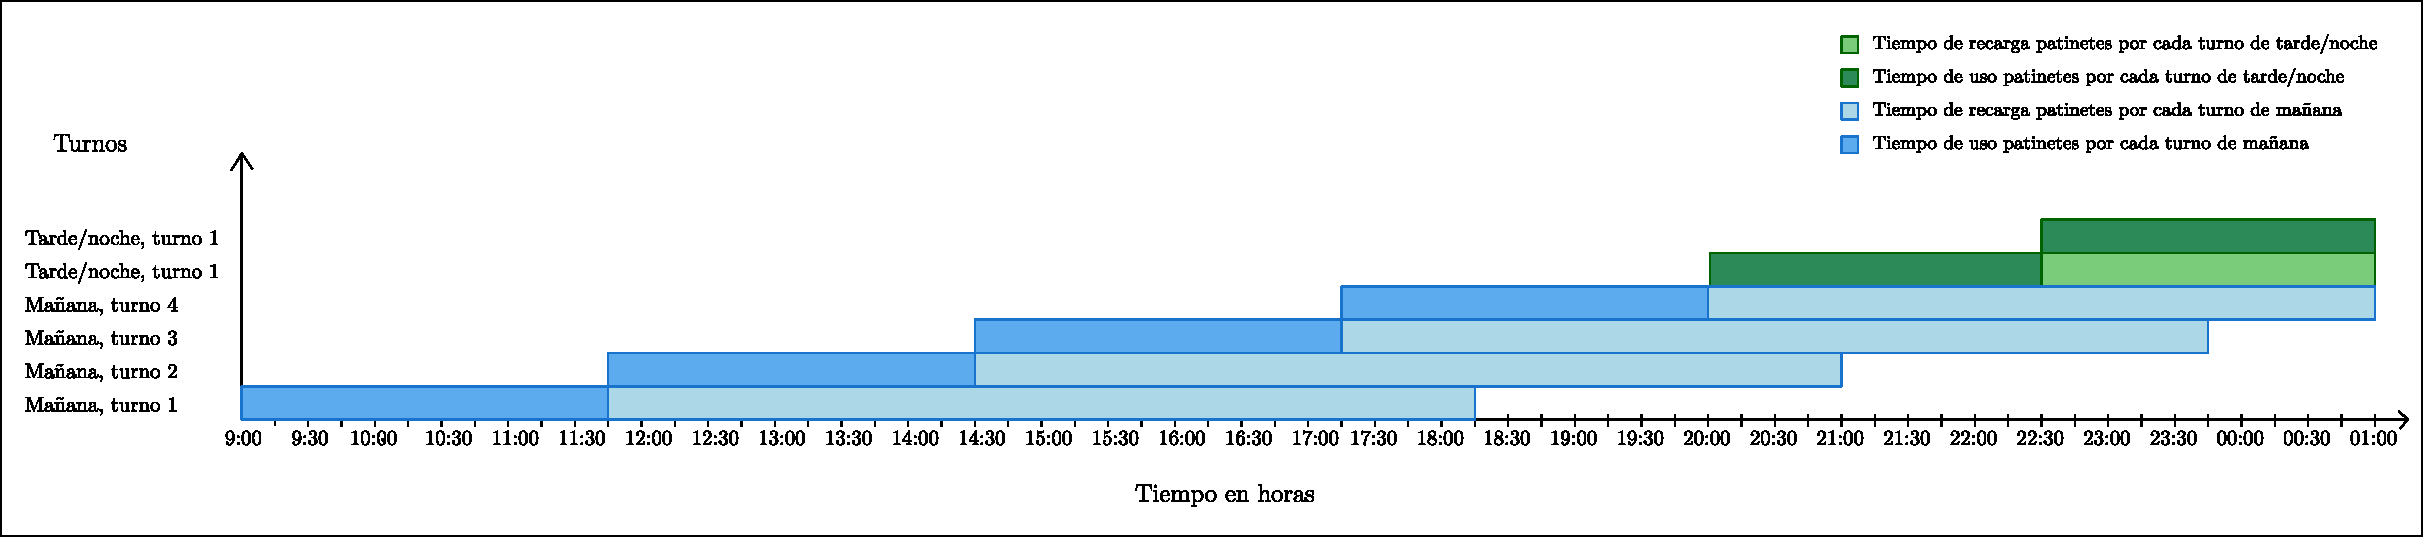
\includegraphics[width= \textwidth, height=12em]{archivos/caso1_patinetes.pdf}
    \caption{Representación turnos de patinetes en viajes de 5 \glssymbol{km}.}
    \label{fig:patinetes_caso1}
\end{figure}

La \autoref{fig:patinetes_caso1} muestra 6 turnos de vehículos, los cuatro primeros en color azul son de 2 vehículos cada uno, lo que implica que se usan 8 patinetes por la mañana. El color verde marca el comienzo del horario de tarde que estará dividido en 2 turnos, cada uno de 7 vehículos. Según el gráfico, cuatro de los vehículos de la mañana se encuentran para el segundo turno de la tarde.

Igualmente, para el supuesto de repartos dobles, recogido en la \autoref{tabla: analisis_detallado_patinete_7.5km}, son reutilizables otros cuatro patinetes, tal como queda reflejado en la
\autoref{fig:patinetes_caso2}.

\begin{figure}[ht]
    \centering
    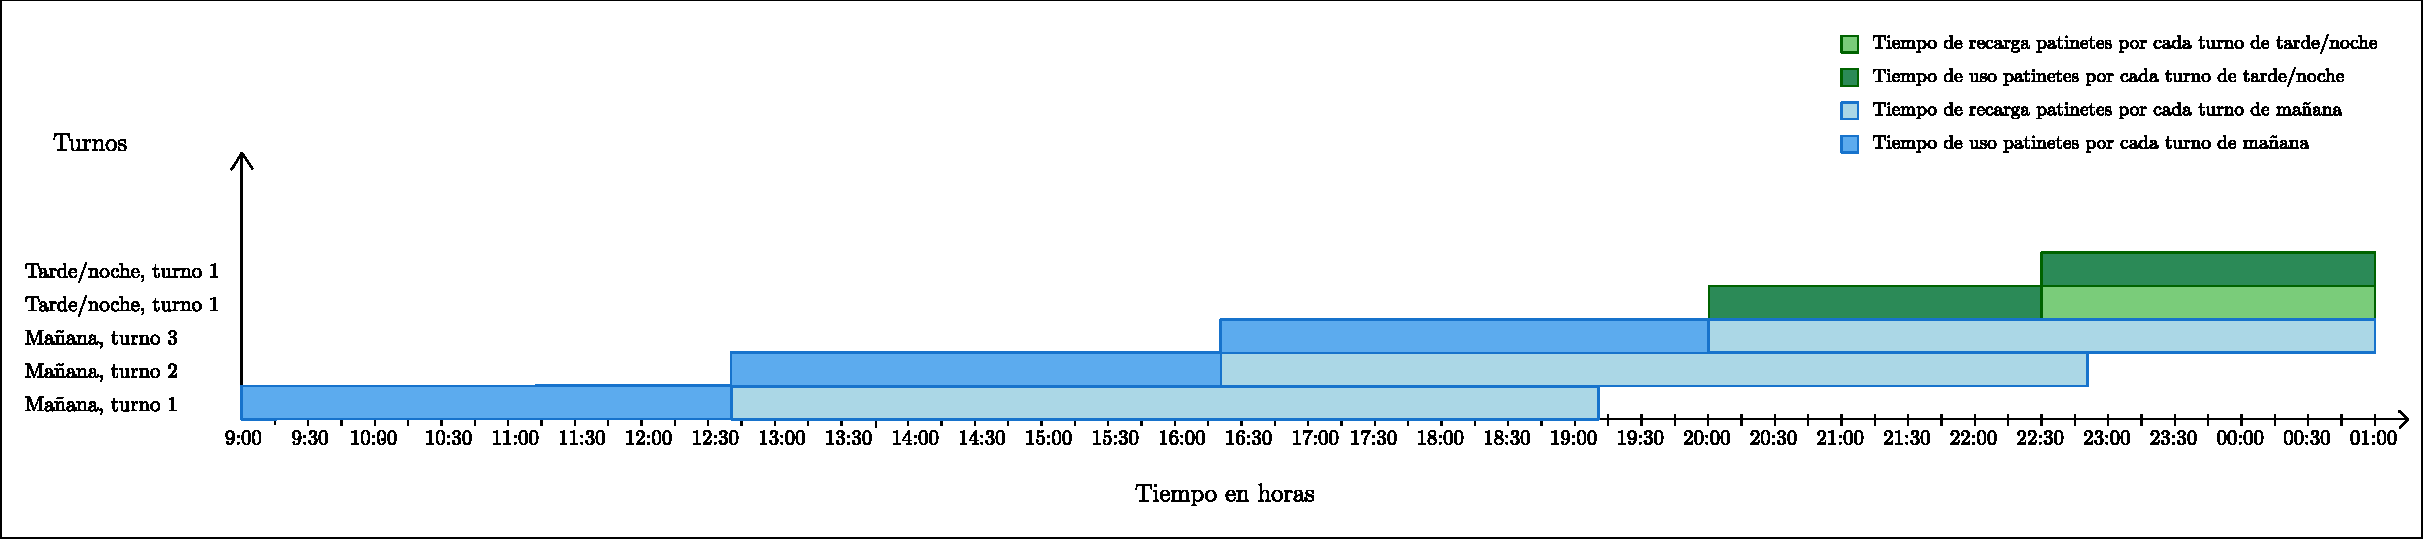
\includegraphics[width= \textwidth, height=12em]{archivos/caso2_patinetes.pdf}
    \caption{Representación turnos de patinetes en viajes de 7,5 \glssymbol{km}.}
    \label{fig:patinetes_caso2}
\end{figure}

Finalmente, se llega a la conclusión que, dada las dos hipótesis de estudios proporcionadas por la empresa, son necesarios veinte patinetes eléctricos en la primera de ellas y, para la segunda, solo dieciséis. Los resultados económicos del análisis de la Infiniton CITYJam Pro quedan reflejados en la \autoref{tab: analisis_presupuestos_patienetes}





% Formula 1
%\begin{equation}
%\label{eqn:ecuacion presupuesto patinete 5km}
 %  11550,11+2817,71*9 = 36.909,5 \text{ \glssymbol{euro}}
%\end{equation}

%\begin{equation}
%\label{eqn: ecuacion presupuesto patinete 7.5km}
%   9327,63+2251,71*9 = 29.593,2 \text{ \glssymbol{euro}}
%\end{equation}



\begin{table}[H]
\centering
\begin{tabular}{|l|c|}
\hline
N.º recargas semanales caso 1 & 136 \\ \hline
N.º recargas semanales caso 2 & 108 \\ \hline
Capacidad batería vehículo (\glssymbol{kilovatiohora}) & 0,35 \\ \hline
Coste recarga unitario (\glssymbol{euro}) & 0,04 \\ \hline
Gasto semanal en  recargas caso 1 (\glssymbol{euro}) & 5,33 \\ \hline
Gasto semanal en  recargas caso 2 (\glssymbol{euro}) & 4,23 \\ \hline
Presupuesto anual en recargas caso 1 (\glssymbol{euro}) & 277,05 \\ \hline
Presupuesto anual en recargas caso 2 (\glssymbol{euro}) & 220,01 \\ \hline
Precio unitario/vehículo (\glssymbol{euro}) & 376,62 \\ \hline
Precio unitario mantenimiento (\glssymbol{euro}) & 124,8 \\ \hline
Reserva de sustitución por vehículo (\glssymbol{euro}) & 20 \\ \hline
Presupuesto para   vehículos primer año caso 1 (\glssymbol{euro}) & 12.323,53 \\ \hline
Presupuesto para vehículos primer año   caso 2 (\glssymbol{euro}) & 9.926,05 \\ \hline
Presupuesto para vehículos anual  caso 1 (\glssymbol{euro}) & 3.873,05 \\ \hline
Presupuesto para vehículos anual caso 2 (\glssymbol{euro}) & 3.096,81 \\ \hline
Presupuesto en vehículos a 10 años, caso 1 (\glssymbol{euro}) & 47.180,97 \\ \hline
Presupuesto en vehículos a 10 años, caso 2 (\glssymbol{euro}) & 37.797,34 \\ \hline
\end{tabular}
\caption{Análisis de los presupuestos patinetes.}
\label{tab: analisis_presupuestos_patienetes}
\end{table}





%\newpage
\section{Motos patinetes electricos}
\label{anexo_motos_patinetes_electricos}

Una vez analizados diversos vehículos factibles para el reparto de comida a domicilio, se ha decidido indagar una alternativa a usar un único vehículo.

En el \autoref{anexo_scooter_electrico} y en el \autoref{anexo_patienete eléctrico} se ha debatido la mejor opción dentro de la gama de motocicletas eléctricas y patinetes eléctricos, respectivamente. En consecuencia, se plantea una alternativa eficiente y coherente que cohesiona a la perfección la autonomía que proporciona el modelo Askoll eS1, con el precio competitivo de las Infiniton CITYJam Pro.

Tomando en consideración que el reparto de los pedidos es homogéneo en todas las franjas horarias, el radio de alcance máximo es de 6 \glssymbol{km}, y la longitud de los pedidos contando ida y vuelta de media oscila entre los 5 y los 7,5 \glssymbol{km}; se puede suponer que la longitud de los recorridos también posee cierta uniformidad. Por ello, se estima que el número de pedidos que se han de repartir en un radio de 4 a 6 km desde el establecimiento, supondrá a lo sumo un 33 (por ciento) de los mismos.

La solución que se plantea es que las motocicletas eléctricas cubran ese porcentaje de pedidos lejanos en todos y cada uno de los tramos horarios estudiados, mientras que los pedidos de corto alcance se realicen en patinetes. De este modo, eliminamos el problema que presentaban los patinetes al no poder alcanzar todas las áreas donde se debían realizar las entregas, al mismo tiempo que se mejora el tiempo de entrega en pedidos cortos porque los patinetes no necesitan ser estacionados, pueden acompañar a su conductor hasta la misma puerta del cliente.

Una motocicleta eléctrica del modelo Askoll eS1 es capaz de realizar unos 100 km a carga completa, lo que equivale a 20 pedidos, suponiendo que los repartos tienen una duración media de 5 km, o 13 pedidos si se suponen 7,5 \glssymbol{km}. Realizando los mismos cálculos que en el \autoref{anexo_calculos_sobre_vehiculos}, pero reduciendo el número de pedidos a realizar en cada tramo horario, se obtiene que son necesarias unos 16 patinetes para la primera hipótesis contemplada (repartos individuales de 5 km) y 14 patinetes para el caso de realizar repartos dobles de 7,5 \glssymbol{km} de ida y vuelta, según la \autoref{tab: analisis_detallado_patinete_5km_2} y la \autoref{tab: analisis_detallado_patinete_7,5km_2}.

\begin{table}[H]
\centering
\begin{tabular}{l|c|c|c|c|}
\cline{2-5}
 & \begin{tabular}[c]{@{}c@{}}TRAMO \\ HORARIO 1\end{tabular} & \begin{tabular}[c]{@{}c@{}}TRAMO \\ HORARIO 2\end{tabular} & \begin{tabular}[c]{@{}c@{}}TRAMO \\ HORARIO 3\end{tabular} & \begin{tabular}[c]{@{}c@{}}TRAMO \\ HORARIO 4\end{tabular} \\ \cline{2-5} 
 & \begin{tabular}[c]{@{}c@{}}Lunes-Jueves \\ (9:00-20:00)\end{tabular} & \begin{tabular}[c]{@{}c@{}}Lunes-Jueves \\ (20:00-0:00)\end{tabular} & \begin{tabular}[c]{@{}c@{}}Viernes-Domingo \\ (9:00-20:00)\end{tabular} & \begin{tabular}[c]{@{}c@{}}Viernes-Domingo \\ (20:00-1:00)\end{tabular} \\ \hline
\multicolumn{1}{|l|}{Nº pedidos} & 30 & 40 & 44 & 90 \\ \hline
\multicolumn{1}{|l|}{\begin{tabular}[c]{@{}l@{}}Distancia total a \\ recorrer \glssymbol{km}\end{tabular}} & 150 & 200 & 220 & 450 \\ \hline
\multicolumn{1}{|l|}{\begin{tabular}[c]{@{}l@{}}Tiempo total de \\ reparto \glssymbol{minuto} \end{tabular}} & 660 & 240 & 660 & 300 \\ \hline
\multicolumn{1}{|l|}{\begin{tabular}[c]{@{}l@{}}Tiempo estimado \\ por pedido (\glssymbol{minuto}/pedido)\end{tabular}} & 20 & 20 & 20 & 20 \\ \hline
\multicolumn{1}{|l|}{\begin{tabular}[c]{@{}l@{}}Nº pedidos realizables \\ por vehículo\end{tabular}} & 33 & 12 & 33 & 15 \\ \hline
\multicolumn{1}{|l|}{\begin{tabular}[c]{@{}l@{}}Nº vehículos simultáneos \\ necesarios\end{tabular}} & 1 & 4 & 2 & 6 \\ \hline
\multicolumn{1}{|l|}{Nº de turnos de vehículos} & 4 & 8 & 3 & 2 \\ \hline
\multicolumn{1}{|l|}{\begin{tabular}[c]{@{}l@{}}Nº vehículos totales \\ necesarios\end{tabular}} & 4 & 8 & 6 & 12 \\ \hline
\end{tabular}
\caption{Análisis detallado del reparto en patinete con viajes de 5 \glssymbol{km}.}
\label{tab: analisis_detallado_patinete_5km_2}
\end{table}



\begin{table}[H]
\centering
\begin{tabular}{l|c|c|c|c|}
\cline{2-5}
 & \begin{tabular}[c]{@{}c@{}}TRAMO \\ HORARIO 1\end{tabular} & \begin{tabular}[c]{@{}c@{}}TRAMO \\ HORARIO 2\end{tabular} & \begin{tabular}[c]{@{}c@{}}TRAMO \\ HORARIO 3\end{tabular} & \begin{tabular}[c]{@{}c@{}}TRAMO \\ HORARIO 4\end{tabular} \\ \cline{2-5} 
 & \begin{tabular}[c]{@{}c@{}}Lunes-Jueves \\ (9:00-20:00)\end{tabular} & \begin{tabular}[c]{@{}c@{}}Lunes-Jueves \\ (20:00-0:00)\end{tabular} & \begin{tabular}[c]{@{}c@{}}Viernes-Domingo \\ (9:00-20:00)\end{tabular} & \begin{tabular}[c]{@{}c@{}}Viernes-Domingo \\ (20:00-1:00)\end{tabular} \\ \hline
\multicolumn{1}{|l|}{Nº pedidos dobles} & 7 & 12 & 17 & 47 \\ \hline
\multicolumn{1}{|l|}{\begin{tabular}[c]{@{}l@{}}Distancia total a \\ recorrer (\glssymbol{km})\end{tabular}} & 52,5 & 90 & 127,5 & 352,5 \\ \hline
\multicolumn{1}{|l|}{\begin{tabular}[c]{@{}l@{}}Tiempo total de \\ reparto doble (\glssymbol{minuto})\end{tabular}} & 660 & 240 & 660 & 300 \\ \hline
\multicolumn{1}{|l|}{\begin{tabular}[c]{@{}l@{}}Tiempo estimado por \\ pedido doble (\glssymbol{minuto}/pedido)\end{tabular}} & 32,5 & 32,5 & 32,5 & 32,5 \\ \hline
\multicolumn{1}{|l|}{\begin{tabular}[c]{@{}l@{}}Nº pedidos dobles \\ realizables por vehículo\end{tabular}} & 20 & 7 & 20 & 9 \\ \hline
\multicolumn{1}{|l|}{\begin{tabular}[c]{@{}l@{}}Nº vehículos simultáneos \\ necesarios\end{tabular}} & 1 & 2 & 1 & 6 \\ \hline
\multicolumn{1}{|l|}{Nº de turnos de vehículos} & 2 & 2 & 4 & 2 \\ \hline
\multicolumn{1}{|l|}{\begin{tabular}[c]{@{}l@{}}Nº vehículos totales \\ necesarios\end{tabular}} & 2 & 4 & 4 & 12 \\ \hline
\end{tabular}
\caption{Análisis detallado del reparto en patinete con viajes de 7,5 \glssymbol{km}.}
\label{tab: analisis_detallado_patinete_7,5km_2}
\end{table}

En la \autoref{fig:patinetes_caso1_2} se comprueba que, efectivamente, 2 de los 6 patinetes empleados en el turno de mañana son reutilizables para el turno de tarde, por lo que como máximo son necesarios 16 patinetes.
\begin{figure}[H]
    \centering
    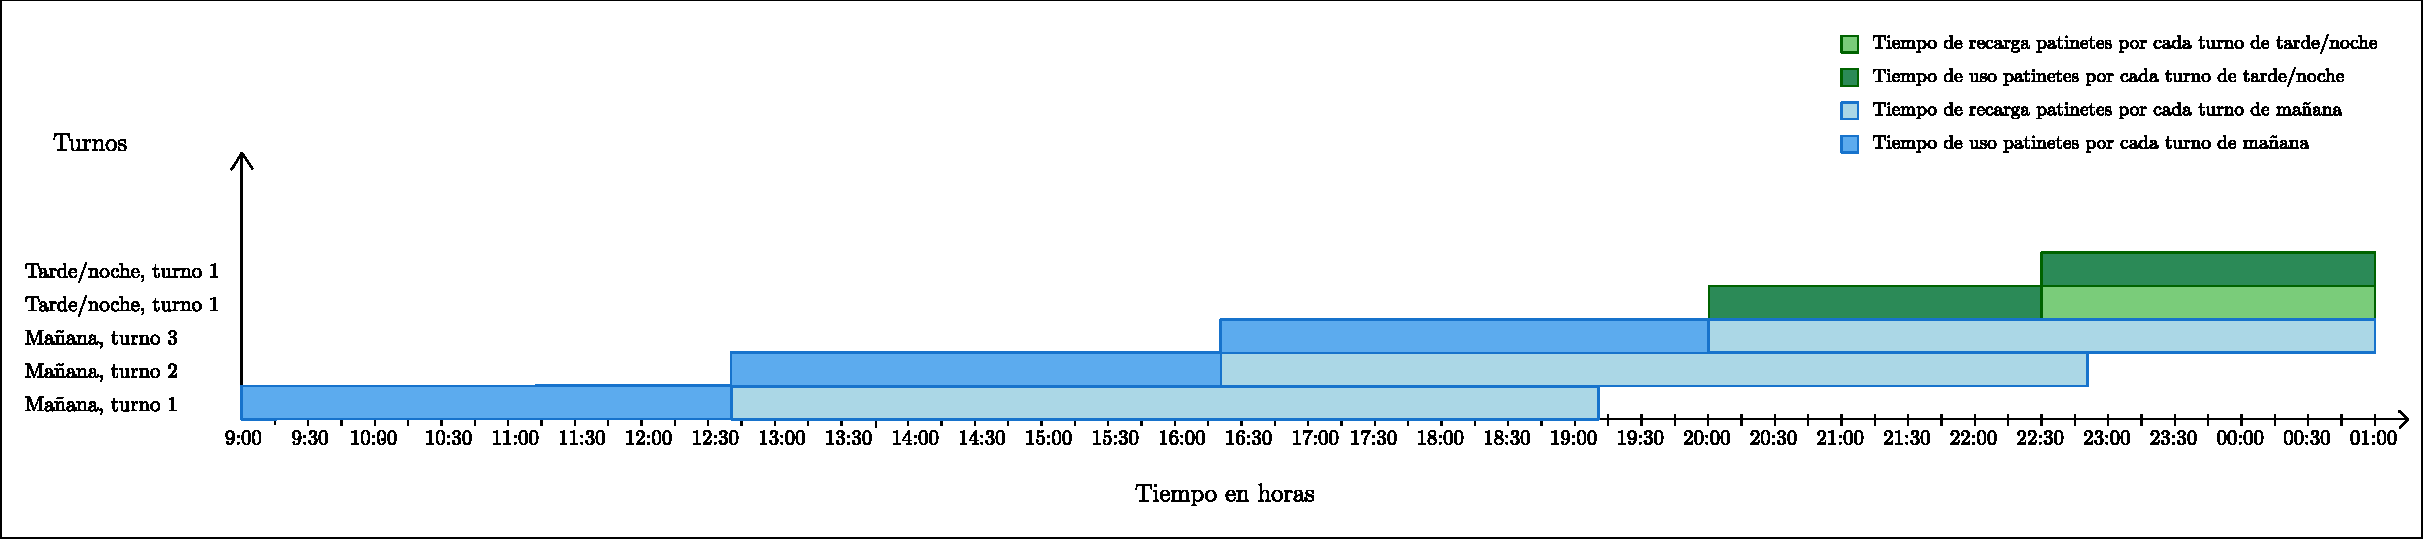
\includegraphics[width= \textwidth, height=12em]{archivos/caso2_patinetes.pdf}
    \caption{Representación turnos minorados de patinetes en viajes de 5 \glssymbol{km}.}
    \label{fig:patinetes_caso1_2}
\end{figure}

Igualmente, en la \autoref{fig:patinetes_caso2_2} se observa que uno de los patinetes se puede recargar y utilizar en el horario posterior, por lo que para esa hipótesis solo son necesarios 14 patinetes.

\begin{figure}[H]
    \centering
    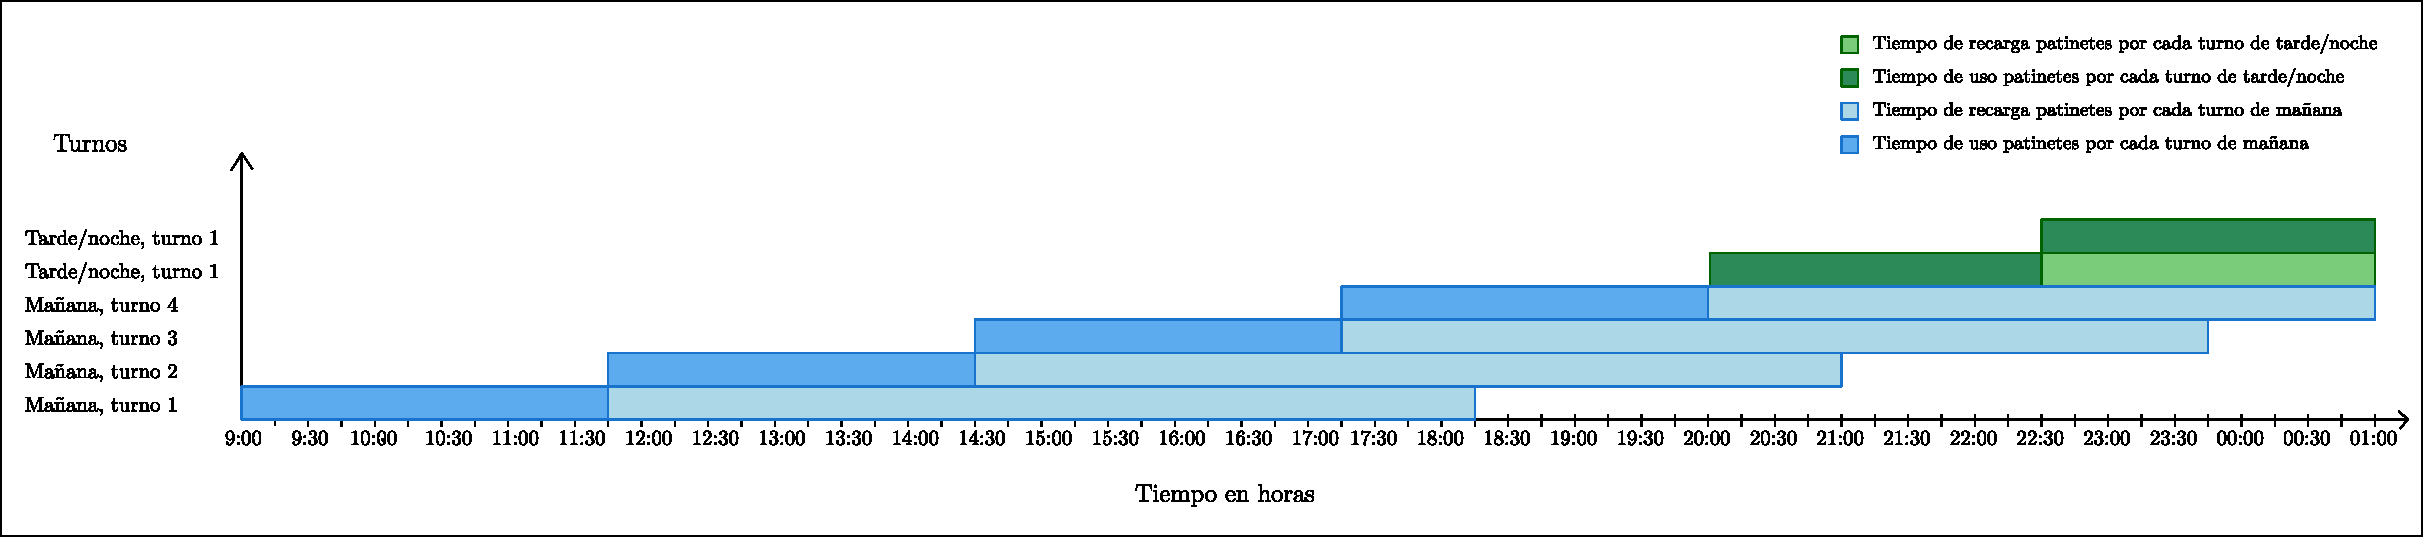
\includegraphics[width= \textwidth, height=12em]{archivos/caso1_patinetes.pdf}
    \caption{Representación turnos minorados de patinetes en viajes de 7,5 \glssymbol{km}.}
    \label{fig:patinetes_caso2_2}
\end{figure}

Finalmente, para hallar el presupuesto de esta opción híbrida se deben tener en cuenta diversos factores. 

Como se ha mencionado anteriormente, se supone  que las motocicletas cubren el 33 (por ciento) de los repartos, por ello los días entre semana se empleará una motocicleta para todo el día, mientras que en los fines de semana se usará una motocicleta en el turno de mañana y en el turno de tarde se ha de emplear la motocicleta del turno anterior además de otra a plena carga.

Respecto a los cálculos se ha de sumar el número de patinetes y sus costes asociados, así como los dos patinetes y sus respectivos costes, todo queda recogido en la \autoref{tab: analisis_presupuestos_patinetes_y_motos}. En estos cálculos se han empleado datos de la \autoref{tabla:tabla_datos_comunes}, de la \autoref{tab: analisis_presupuestos_patienetes} y de la \autoref{tab:Estudio presupuestos modelo Askoll eS1} debido a que estos modelos ya se han analizado en detalle en el \autoref{anexo_calculos_sobre_vehiculos}.

\begin{table}[H]
\centering
\begin{tabular}{|l|c|}
\hline
Nº recargas semanales patinetes caso 1 & 102 \\ \hline
Nº recargas semanales patinetes caso 2 & 72 \\ \hline
Nº recargas semanales motocicletas caso 1 & 10 \\ \hline
Nº recargas semanales motocicletas caso 2 & 10 \\ \hline
Presupuesto anual en recargas caso 1 (\glssymbol{euro}) & 330,01 \\ \hline
Presupuesto anual en recargas caso 2 (\glssymbol{euro}) & 268,90 \\ \hline
Presupuesto para vehículos primer año caso 1 (\glssymbol{euro}) & 16.536,67 \\ \hline
Presupuesto para vehículos primer año   caso 2 (\glssymbol{euro}) & 15.362,72 \\ \hline
Presupuesto para vehículos anual  caso 1 (\glssymbol{euro}) & 4.205,91 \\ \hline
Presupuesto para vehículos anual caso 2 (\glssymbol{euro}) & 3.785,20 \\ \hline
Presupuesto en vehículos a 10 años, caso 1 (\glssymbol{euro}) & 54.389,9 \\ \hline
Presupuesto en vehículos a 10 años, caso 2 (\glssymbol{euro}) & 49.429,53 \\ \hline
\end{tabular}
\caption{Análisis de los presupuestos opción óptima.}
\label{tab: analisis_presupuestos_patinetes_y_motos}
\end{table}



\newpage
\section{Precio de talleres y combustible}
\label{anexo_precio_taller_combustible}

Una motocicleta necesita un mantenimiento cada cierto tiempo o kilometraje, al año se estima que se necesitan los mantenimientos de la \autoref{tabla: reparaciones y precios} y su coste.

\begin{table}[H]
\centering
\begin{tabular}{|c|c|c|}
\hline
                           & \textbf{Nº veces/año} & \textbf{Coste total (\glssymbol{euro})} \\ \hline
\textbf{Cambios de aceite} & 1                     & 80                   \\ \hline
\textbf{Revisiones}        & 0,33                  & 66                   \\ \hline
\textbf{Ruedas}            & 0,5                   & 40                   \\ \hline
\textbf{Frenos}            & 0,5                   & 20                   \\ \hline
\textbf{Transmisión}       & 0,33                  & 33                   \\ \hline
\textbf{TOTAL}             &                       & \textbf{239}                 \\ \hline
\end{tabular}
\caption{Reparaciones y precios de motocicletas y ciclomotores.}
\label{tabla: reparaciones y precios}
\end{table}

El mantenimiento de las motos eléctricas no resulta tan caro en comparación a las de gasolina, resultando en 126 \glssymbol{euro}.

El mantenimiento de un patinete es más económico, tal y como se observa en la \autoref{tab: Reparaciones y precios patinetes} \cite{tarifaspatinete1}, considerando que tiene componentes electrónicos que pueden hacer más elevado su precio.

\begin{table}[H]
\centering
\begin{tabular}{|l|l|}
\hline
\textbf{}                               & \multicolumn{1}{c|}{\textbf{Precio (\glssymbol{euro})}} \\ \hline
\textbf{Cambio de 2 ruedas 10 pulgadas} & 25                                  \\ \hline
\textbf{Luces, acelarador, dirección}   & 8,95                                  \\ \hline
\textbf{Ajuste de frenos}               & 15,95                                 \\ \hline
\textbf{Cambio de batería}              & 34,95                                 \\ \hline
\textbf{Suspensión}                     & 39,95                                 \\ \hline
\textbf{Total}                          & \textbf{124,8}                       \\ \hline
\end{tabular}
\caption{Reparaciones y precios de patinetes.}
\label{tab: Reparaciones y precios patinetes}
\end{table}


Para garantizar tener capital de respaldo para sustituir un vehículo entero en caso de siniestro, se le suman a los patinetes y a las motos un respaldo que permitan ahorrar para su sustitución, de 20 \gls{euro} y 100 \gls{euro} anuales por vehículo respectivamente.


Por otro lado, el valor del precio de la electricidad y gasolina se ha obtenido mediante los datos diarios del año anterior al presente \cite{historicoluz,historicocombustible}. Sus representaciones gráficas sobre la fluctuación de mercado, tal y como se muestran en la \autoref{fig:precio luz 2021} y \autoref{fig:precio gasolina 2021}, siendo el precio medio de la gasolina de 1,38 \glssymbol{euro}/\glssymbol{litros}, y el de la luz de 111,93 \glssymbol{euro}/MWh.

\begin{figure}[H]
    \centering
    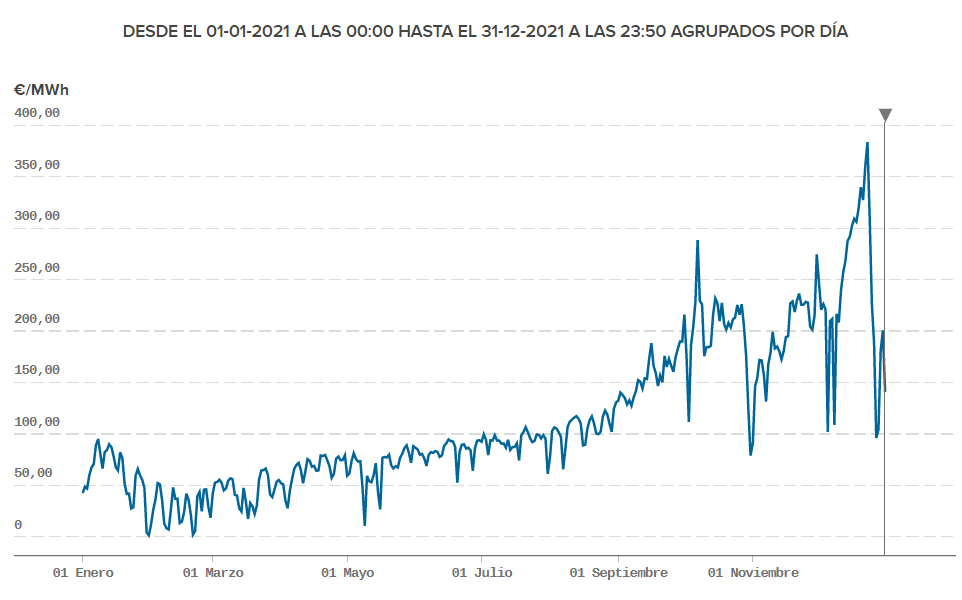
\includegraphics[scale=0.4]{archivos/precio luz 2021.png}
    \caption{Histórico precio electricidad.}
    \label{fig:precio luz 2021}
\end{figure}

\begin{figure}[H]
    \centering
    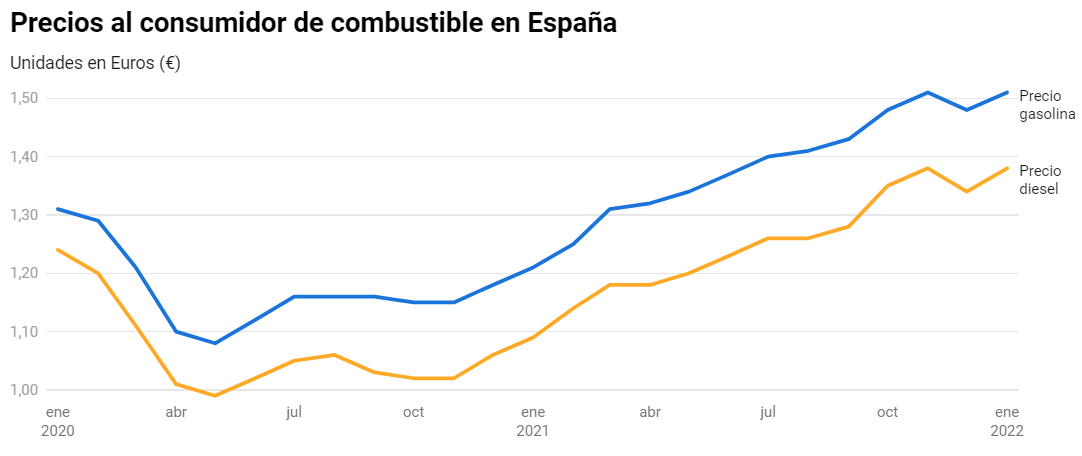
\includegraphics[scale=0.35]{archivos/precio gasolina 2021.png}
    \caption{Histórico precio combustible.}
    \label{fig:precio gasolina 2021}
\end{figure}

\newpage
% \addcontentsline{toc}{section}{Referencias}
% \section*{Referencias}
% \label{referencias_nucleo}
% \makeatletter
% \def\@bibitem#1{\item\if@filesw \immediate\write\@auxout
%   {\string\bibcite{#1}{A\the\value{\@listctr}}}\fi\ignorespaces}
% \def\@biblabel#1{[A{#1}]}
% \makeatother
% \printbibheading[title={Referencias},heading=bibintoc]
\nocite{*}
\newrefcontext[labelprefix=\thesection.]
\printbibheading[title={Referencias},heading=subbibintoc]
\printbibliography[heading=none,resetnumbers=true,keyword=preciotaller]
\section{Fichas técnicas}
\label{anexo:ficha tecnica}

\subsection{Ficha técnica KYMCO Agility Carry 50 E5}
\label{subanexo: ficha tecnica kymco 50}

\begin{figure}[H]
    \centering
    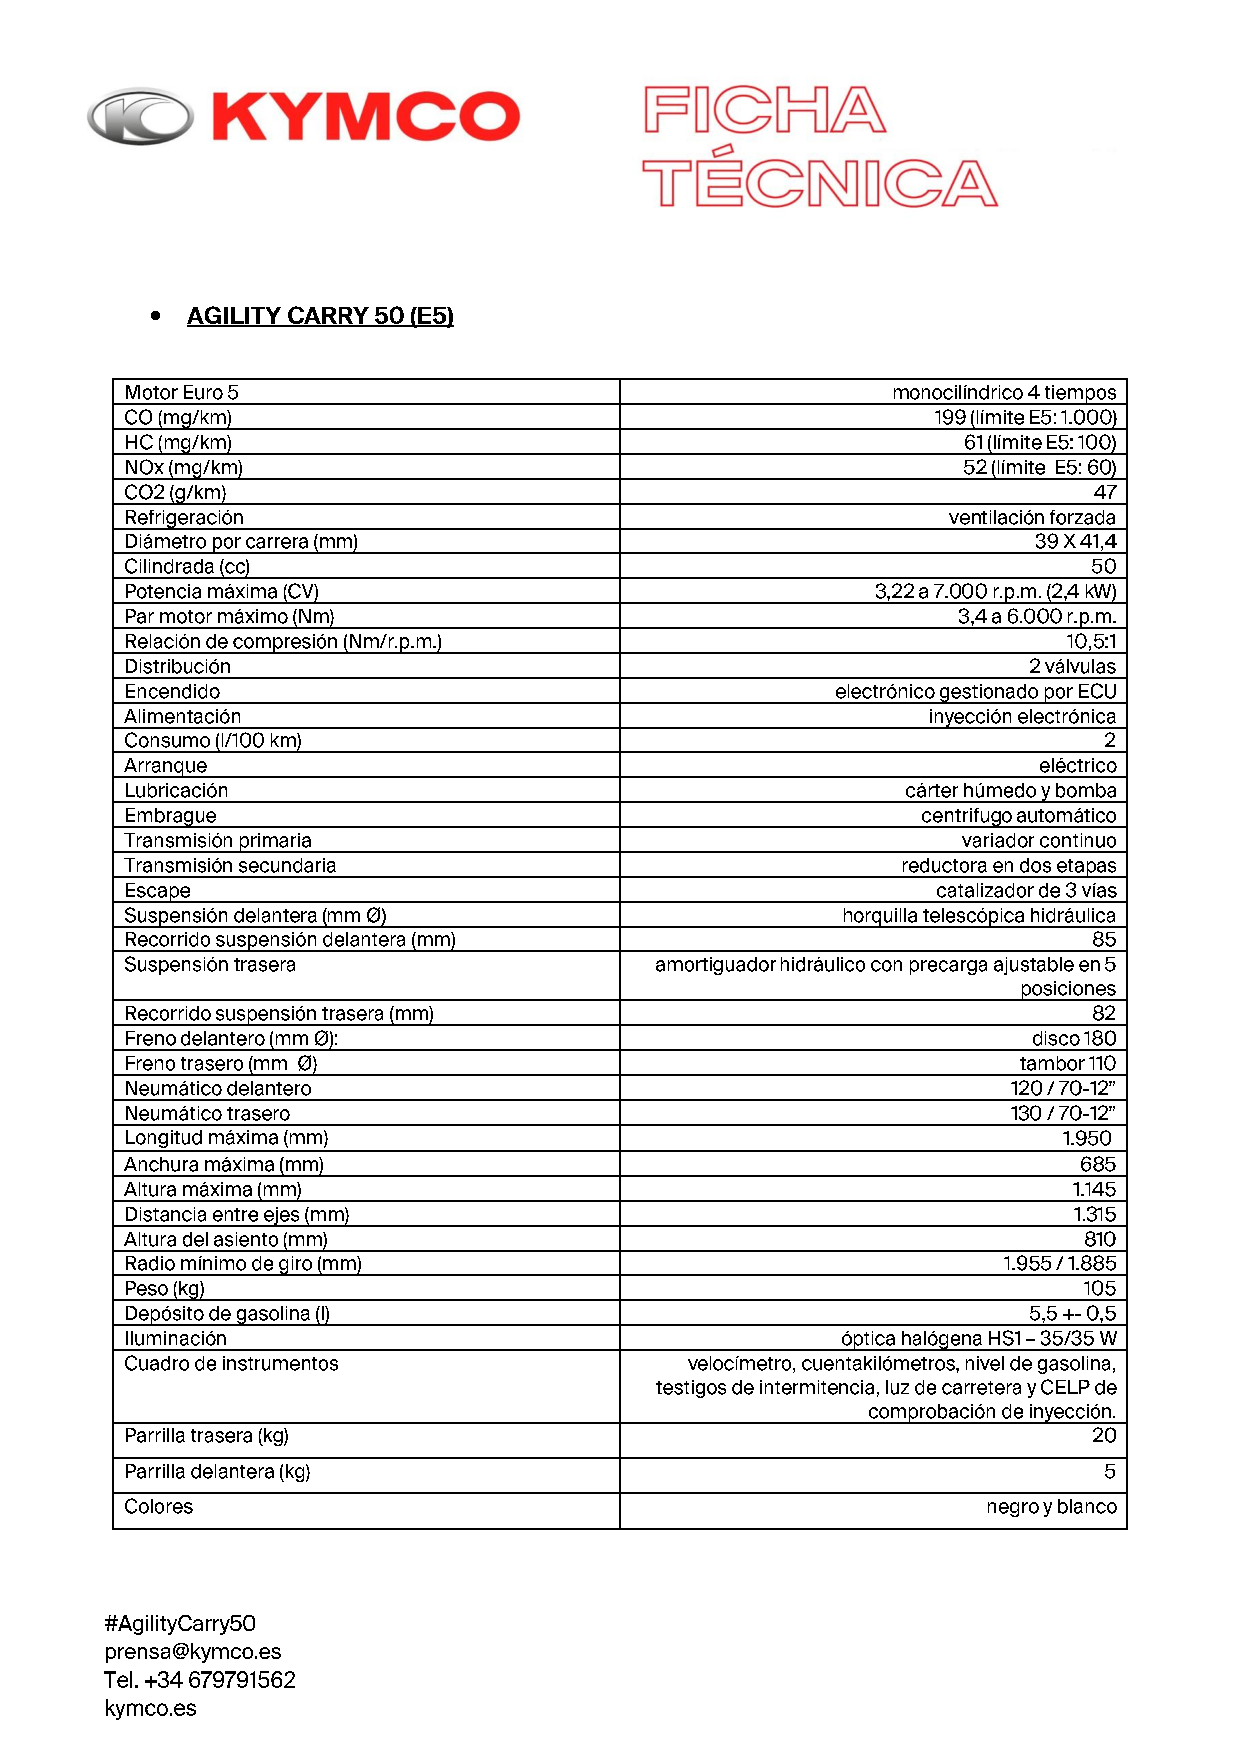
\includegraphics[scale = 0.7]{archivos/ficha_tecnica_motillo_peter.pdf}
    \caption{Ficha Técnica KYMCO Agility Carry 50 E5.}
    \label{fig: ficha tecnica KYMCO 50}
\end{figure}

%Jorge, encuentrame

\subsection{Ficha técnica KYMCO Agility Carry 125}
\label{subanexo: ficha tecnica kymco 125}

\begin{table}[H]
\centering
\begin{tabular}{l}
\multicolumn{1}{c}{\textbf{Datos comerciales KYMCO Agility Carry 125 2021-2022}} \\ \hline
\textbf{Marca:}                  \\
KYMCO                            \\
\textbf{Tipo de carnet:}         \\
125cc                            \\
\textbf{Año:}                    \\
2021                             \\
\textbf{Plazas:}                 \\
1                                \\
                                 \\
\multicolumn{1}{c}{\textbf{Motor y transmisión}}                                 \\ \hline
\textbf{Cilindrada exacta:}      \\
125 cc                           \\
\textbf{Tipo:}                   \\
4 T                              \\
\textbf{Distribución:}           \\
SOHC                             \\
\textbf{Cilindros:}              \\
1                                \\
\textbf{Válvulas por cilindro:}  \\
2                                \\
\textbf{Alimentación:}           \\
Inyección electrónica            \\
\textbf{Refrigeración:}          \\
Aire forzado                     \\
\textbf{Diámetro por carrera:}   \\
52.4 mm x 57.8 mm                \\
\textbf{Compresión:}             \\
9.6 :1                           \\
\textbf{Potencia máxima declarada:}                                              \\
9.12 CV a 7.500 rpm              \\
\textbf{Combustible:}            \\
Gasolina sin plomo 95            \\
\textbf{Normativa anticontaminación:}                                            \\
Euro5                            \\
\textbf{Encendido:}              \\
Electrónico CDI                  \\
\textbf{Transmisión secundaria:} \\
Correa                           \\
\textbf{Embrague:}               \\
Automático centrífugo en seco   
\end{tabular}
\end{table}

\begin{table}[H]
\centering
\begin{tabular}{lll}
\multicolumn{1}{c}{\textbf{Suspensión delantera}} &  & \multicolumn{1}{c}{\textbf{Suspensión trasera}} \\ \cline{1-1} \cline{3-3} 
\textbf{Tipo de suspensión delantera:}       &  & \textbf{Tipo basculante:}                       \\
Horquilla telescópica                        &  & Motor                                           \\
\textbf{Diámetro de barras:}                 &  & \textbf{Tipo de suspensión trasera:}            \\
31 mm                                        &  & Doble amortiguador                              \\
\textbf{Recorrido:}                          &  & \textbf{Recorrido:}                             \\
85 mm                                        &  & 82 mm                                           \\
\textbf{}                                    &  & \textbf{Regulaciones:}                          \\
\multicolumn{1}{c}{\textbf{}}                &  & Cinco puntos de precarga                        \\
\textbf{}                                    &  & \textbf{}                                       \\
\multicolumn{1}{c}{\textbf{Freno delantero}} &  & \multicolumn{1}{c}{\textbf{Freno trasero}}      \\ \cline{1-1} \cline{3-3} 
\textbf{Sistema:}                            &  & \textbf{Sistema:}                               \\
Disco (CBS)                                  &  & Disco                                           \\
\textbf{Diámetro:}                           &  & \textbf{Diámetro:}                              \\
220 mm                                       &  & 200 mm                                          \\
\textbf{Pinza:}                              &  & \textbf{}                                       \\
3 pistones                                   &  & \multicolumn{1}{c}{\textbf{}}                   \\
\textbf{}                                    &  & \textbf{}                                       \\
\multicolumn{1}{c}{\textbf{Rueda delantera}} &  & \multicolumn{1}{c}{\textbf{Rueda trasera}}      \\ \cline{1-1} \cline{3-3} 
\textbf{Diámetro de llanta:}                 &  & \textbf{Diámetro de llanta:}                    \\
12 "                                         &  & 12 "                                            \\
\textbf{Marca de neumáticos:}                &  & \textbf{Marca de neumáticos:}                   \\
CST                                          &  & CST                                             \\
\textbf{Medida de neumáticos:}               &  & \textbf{Medida de neumáticos:}                  \\
120/70-12                                    &  & 130/70-12                                       \\
\textbf{}                                    &  &                                                 \\
\textbf{}                                    &  & \textbf{}                                       \\
\multicolumn{1}{c}{\textbf{Chasis}}          &  & \multicolumn{1}{c}{\textbf{Dimensiones y peso}} \\ \cline{1-1} \cline{3-3} 
\textbf{Tipo de chasis:}                     &  & \textbf{Longitud máxima:}                       \\
Tubular                                      &  & 1.925 mm                                        \\
                                             &  & \textbf{Anchura máxima:}                        \\
\textbf{}                                    &  & 695 mm                                          \\
\textbf{}                                    &  & \textbf{Altura máxima:}                         \\
\textbf{}                                    &  & 1.100 mm                                        \\
\textbf{}                                    &  & \textbf{Distancia entre ejes:}                  \\
\textbf{}                                    &  & 1.310 mm                                        \\
\textbf{}                                    &  & \textbf{Altura de asiento:}                     \\
\textbf{}                                    &  & 790 mm                                          \\
                                             &  & \textbf{Ángulo de dirección:}                   \\
\textbf{}                                    &  & 40 º                                            \\
\textbf{}                                    &  & \textbf{Capacidad del depósito:}                \\
\textbf{}                                    &  & 6,5 l.                                          \\
\textbf{}                                    &  & \textbf{Peso en seco:}                          \\
\textbf{}                                    &  & 123 Kg                                         
\end{tabular}
\caption{Ficha Técnica KYMCO Agility Carry 125.}
\label{tab: ficha tecnica KYMCO}
\end{table}




\subsection{Ficha técnica Askoll eS1}
\label{subanexo: ficha tecnica askill es1}

\begin{table}[H]
\centering
\begin{tabular}{lll}
\multicolumn{3}{c}{\textbf{Datos comerciales Askoll eS1 2021-2022}}                \\\cline{1-3}
\multicolumn{1}{c}{\textbf{Motor, prestaciones y consumo}} &  & \multicolumn{1}{c}{\textbf{Batería}}                       \\ \cline{1-1} \cline{3-3} 
\textbf{Tipo de motor:}             &  & \textbf{Tipo de batería:}                 \\
Eléctrico sin escobillas Askoll de imanes permanentes      &  & Iones de litio 54 V - 20 Ah                                \\
\textbf{Potencia máxima CV:}        &  & \textbf{Capacidad:}                       \\
2 CV                                &  & 2.1 kWh                                   \\
\textbf{Potencia máxima kW:}        &  & \textbf{Extraíble:}                       \\
1.5 kW/rpm                          &  & SI                                        \\
\textbf{Velocidad máxima:}          &  & \textbf{Tipo de carga / Tiempo 100\%:}    \\
45 km/h                             &  & 3 horas                                   \\
\textbf{Autonomía en ciudad:}       &  & \textbf{Vida/Ciclos de carga hasta 80\%:} \\
100 km                              &  & 800 ciclos                                \\
\multicolumn{1}{c}{\textbf{}}       &  &                                           \\
\multicolumn{1}{c}{\textbf{Chasis}} &  &                                           \\ \cline{1-1}
\textbf{Suspensión delantera:}                             &  & \multicolumn{1}{c}{\textbf{Dimensiones, peso y capacidad}} \\ \cline{3-3} 
Horquilla telescópica hidráulica    &  & \textbf{Altura:}                          \\
\textbf{Suspensión trasera:}        &  & 760 mm al asiento mm                      \\
Amortiguador hidráulico             &  & \textbf{Peso total:}                      \\
\textbf{Frenos delanteros:}         &  & 72 kg                                     \\
Hidráulico - de disco Ø 190 mm      &  & \textbf{Número de plazas:}                \\
\textbf{Frenos traseros:}           &  & 1                                         \\
Tambor Ø 140 mm                     &  &                                           \\
\textbf{Neumático delantero:}       &  & \multicolumn{1}{c}{\textbf{Transmisión}}  \\ \cline{3-3} 
80 / 80 - 16                        &  & \textbf{Tracción:}                        \\
\textbf{Neumático trasero:}         &  & Polea con correa dentada                  \\
90 / 80 - 16                        &  &                                          
\end{tabular}
\caption{Ficha Técnica Askoll eS1.}
\label{tab: ficha tecnica askoll}
\end{table}


\newpage
\subsection{Ficha técnica Infiniton CityJam Pro}
\label{subanexo: ficha tecnica infinity cityjam}

\begin{table}[H]
\centering
\begin{tabular}{lll}
\multicolumn{3}{c}{\textbf{Infiniton CityJam Pro}}                        \\ \hline
\textbf{Velocidad máxima:}          &           & \textbf{Potencia:}      \\
25 km/h                             &           & 350 W                   \\
\textbf{Autonomía:}                 &           & \textbf{Peso máximo:}   \\
40 - 45 km                          &           & 100 kg                  \\
\textbf{Pendiente máxima:}          &           & \textbf{App móvil:}     \\
15º                                 & \textbf{} & SI                      \\
\textbf{Tipo de batería}            &           & \textbf{Display LED:}   \\
Litio                               &           & SI                      \\
\textbf{Freno delantero y trasero:} &           & \textbf{Luz LED:}       \\
SMART BRAKE                         &           & Frontal                 \\
\textbf{Suspensión delantera:}      &           & \textbf{Revestimiento:} \\
FULLY SOFT                          &           & IP54                    \\
\textbf{Modos de conducción:}       &           & \textbf{Plegable:}      \\
Sport - ECO - Crucero               &           & SI                      \\
\textbf{Medidas:}                   &           &                         \\
1130x455x1220 mm                    &           &                        
\end{tabular}
\caption{Ficha Técnica Infinity CityJam Pro.}
\label{tab: ficha tecnica infinity cityjam}
\end{table}

%\newpage
\section{Ficha técnica Askoll eS1}
\label{anexo:ficha tecnica askoll}


\begin{table}[H]
\centering
\begin{tabular}{lll}
\multicolumn{3}{c}{\textbf{Datos comerciales Askoll eS1 2021-2022}}                \\\cline{1-3}
\multicolumn{1}{c}{\textbf{Motor, prestaciones y consumo}} &  & \multicolumn{1}{c}{\textbf{Batería}}                       \\ \cline{1-1} \cline{3-3} 
\textbf{Tipo de motor:}             &  & \textbf{Tipo de batería:}                 \\
Eléctrico sin escobillas Askoll de imanes permanentes      &  & Iones de litio 54 V - 20 Ah                                \\
\textbf{Potencia máxima CV:}        &  & \textbf{Capacidad:}                       \\
2 CV                                &  & 2.1 kWh                                   \\
\textbf{Potencia máxima kW:}        &  & \textbf{Extraíble:}                       \\
1.5 kW/rpm                          &  & SI                                        \\
\textbf{Velocidad máxima:}          &  & \textbf{Tipo de carga / Tiempo 100\%:}    \\
45 km/h                             &  & 3 horas                                   \\
\textbf{Autonomía en ciudad:}       &  & \textbf{Vida/Ciclos de carga hasta 80\%:} \\
100 km                              &  & 800 ciclos                                \\
\multicolumn{1}{c}{\textbf{}}       &  &                                           \\
\multicolumn{1}{c}{\textbf{Chasis}} &  &                                           \\ \cline{1-1}
\textbf{Suspensión delantera:}                             &  & \multicolumn{1}{c}{\textbf{Dimensiones, peso y capacidad}} \\ \cline{3-3} 
Horquilla telescópica hidráulica    &  & \textbf{Altura:}                          \\
\textbf{Suspensión trasera:}        &  & 760 mm al asiento mm                      \\
Amortiguador hidráulico             &  & \textbf{Peso total:}                      \\
\textbf{Frenos delanteros:}         &  & 72 kg                                     \\
Hidráulico - de disco Ø 190 mm      &  & \textbf{Número de plazas:}                \\
\textbf{Frenos traseros:}           &  & 1                                         \\
Tambor Ø 140 mm                     &  &                                           \\
\textbf{Neumático delantero:}       &  & \multicolumn{1}{c}{\textbf{Transmisión}}  \\ \cline{3-3} 
80 / 80 - 16                        &  & \textbf{Tracción:}                        \\
\textbf{Neumático trasero:}         &  & Polea con correa dentada                  \\
90 / 80 - 16                        &  &                                          
\end{tabular}
\caption{Ficha Técnica Askoll eS1.}
\label{tab: ficha tecnica askoll}
\end{table}
%\newpage
\section{Ficha técnica Askoll eS1}
\label{anexo:ficha tecnica infinity cityjam}

\begin{table}[H]
\centering
\begin{tabular}{lll}
\multicolumn{3}{c}{\textbf{Infiniton CityJam Pro}}                        \\ \hline
\textbf{Velocidad máxima:}          &           & \textbf{Potencia:}      \\
25 km/h                             &           & 350 W                   \\
\textbf{Autonomía:}                 &           & \textbf{Peso máximo:}   \\
40 - 45 km                          &           & 100 kg                  \\
\textbf{Pendiente máxima:}          &           & \textbf{App móvil:}     \\
15º                                 & \textbf{} & SI                      \\
\textbf{Tipo de batería}            &           & \textbf{Display LED:}   \\
Litio                               &           & SI                      \\
\textbf{Freno delantero y trasero:} &           & \textbf{Luz LED:}       \\
SMART BRAKE                         &           & Frontal                 \\
\textbf{Suspensión delantera:}      &           & \textbf{Revestimiento:} \\
FULLY SOFT                          &           & IP54                    \\
\textbf{Modos de conducción:}       &           & \textbf{Plegable:}      \\
Sport - ECO - Crucero               &           & SI                      \\
\textbf{Medidas:}                   &           &                         \\
1130x455x1220 mm                    &           &                        
\end{tabular}
\caption{Ficha Técnica Infinity CityJam Pro}
\label{tab: ficha tecnica infinity cityjam}

\end{table}
\newpage
\section{Cálculos sobre infraestructuras}
\label{anexo:infraestructuras}

Los cálculos de la construcción de la infraestructura dependen de muchos factores, entre ellos la fecha de la obra o el tiempo máximo que pueda durar, así como sus dimensiones son factores que llegan a afectar mucho al precio de la misma. Por ello se considerará que ante la ausencia de un plano del local se realizará una estimación aproximada del coste de la obra, por ello se tomará como referencia un precio medio que se puede encontrar en las páginas web de las empresas FIXr \cite{fixr} y Zaask \cite{zaask} puesto que coincide con lo que se ha encontrado durante la investigación y se puede considerar una buena aproximación a lo que sería el precio final de la obra.

\subsection{Cálculo del precio de los accesorios específicos}

\textbf{\textit{Puesto que estos cálculos son necesarios para los siguientes, se realizarán primero.}}

Debido a motivos de seguridad se considera necesario la instalación de ciertos mecanismos de seguridad definidos a continuación.

\subsubsection{Bicicletas Eléctricas}
En el caso de las bicicletas eléctricas se considera que es necesario instalar algún tipo de estructura donde poder encadenarlas y así evitar posibles robos. Se ha escogido el modelo \textbf{Soporte 5 bicicletas} de la marca \textbf{Btwin} (Decatlon) \cite{decathlons5b}, porque se considera que es el que mejor se adapta a nuestras necesidades manteniendo una buena relación calidad/precio, con un coste de 54,99 \glssymbol{euro} por unidad.

También se debe contar con el precio del candado, se ha escogido como mejor opción el \textbf{Candado para bicicletas en U 920 Elops} de la marca \textbf{Elops} \cite{decathloncb}, por su facilidad de uso, por contar con un soporte para la bicicleta (que asegura que no pueda molestar al repartidor) y por su buena relación calidad/precio, que supone un coste de 29,99 \glssymbol{euro} por unidad.

\subsubsection{Patinetes Eléctricos}
En el caso de los patinetes eléctricos se considera necesario instalar una estructura para poder encadenarlos, al igual que con las bicicletas, en este caso la opción que se ha considerado óptima se trata del \textbf{Aparcapatinetes Manuales} de la marca \textbf{Adosa} \cite{aparcapatinetes} (por desgracia el mercado de los patinetes eléctricos es relativamente reciente y por ello el precio en comparación con los soportes para bicicletas es mucho mas elevado) de un precio de 288,61 \glssymbol{euro} para un soporte de  \textbf{8 patinetes}.

También se debe contar con el candado, en este caso se ha escogido el candado \textbf{Masterlock candado-esposas patinete negro} de la marca \textbf{Master Lock} pues se considera es el que mejor se adapta a las necesidades con una buena relación calidad/precio, con un coste de 28,99 \glssymbol{euro} por unidad.


\subsection{Cálculo del área necesaria para cada vehículo}

En todos los casos se considera que el acceso desde la calle hasta el aparcamiento ocupará un total de 4 \glssymbol{metrocuadrado} como máximo, así como un espacio de maniobra de 1,5 \glssymbol{metro} en el caso de las motocicletas, y de 1 \glssymbol{metro} en el caso de patinetes eléctricos y bicicletas eléctricas.

\subsubsection{Motocicletas}
Para el calculo del espacio necesario para las motocicletas, y teniendo en cuenta que en las ordenanzas municipales de la ciudad de Málaga \cite{ordmalaga} no se especifica un tamaño mínimo o necesario para el estacionamiento de ciclomotores, se definirá el tamaño de este en relación a cada vehículo que se vaya a aparcar, añadiendo 15 \glssymbol{centimetro} hacia cada lateral del vehículo, para permitir un mínimo de movilidad entre los vehículos, más la distancia de maniobra anteriormente mencionada.

\paragraph{Askoll eS1:}
\label{askolles1}

Medidas: 1830 x 726 x 1036 \glssymbol{milimetro}. \cite{manualmotoe}

Considerando los 15 \glssymbol{centimetro} hacia cada lateral, más 1,5 \glssymbol{metro} de espacio de maniobra, se puede considerar un área total por vehículo de 3330 x 1026 \glssymbol{milimetro}.

\paragraph{KYMCO Agility Carry 50 E5}
\label{agilitycarry50}

Medidas: 1950 x 1145 x 685 \glssymbol{milimetro}. \cite{eliotmotor}

Considerando los 15 \glssymbol{centimetro} hacia cada lateral, más 1,5 \glssymbol{metro} de espacio de maniobra, se puede considerar un área total por vehículo de 3430 x 1445 \glssymbol{milimetro}.

\paragraph{KYMCO AGility Carry 125}
\label{agilitycarry125}

Medidas: 1925 x 695 x 1100 \glssymbol{milimetro}. \cite{motofichas}

Considerando los 15 \glssymbol{centimetro} hacia cada lateral, más 1,5 \glssymbol{metro} de espacio de maniobra, se puede considerar un área total por vehículo de 3425 x 995 \glssymbol{milimetro}.

\subsubsection{Bicicletas Eléctricas}
\label{bicicletaselectricas}

El cálculo del espacio necesario para las bicicletas eléctricas se debe basar en el espacio que ocupará el soporte de estas (definido más abajo), más el tamaño de la propia bicicleta, más el espacio de maniobra.

En el caso del soporte el modelo escogido se cuenta con unas dimensiones de \cite{aparcapatinetes} 1357 x 375 x 250 \glssymbol{milimetro}

En el caso de la bicicleta eléctrica escogida se cuenta con unas medidas de \cite{emoonmedidas}  188 x 117 x 21 \glssymbol{centimetro}

Teniendo en cuenta que se instalará un soporte para bicicletas las medidas a tener en cuenta son 1357 \glssymbol{milimetro} de ancho, 188 \glssymbol{centimetro} de la bicicleta (se considera el soporte despreciable en esta dirección) más 1 \glssymbol{metro} reservado para maniobras de largo, por cada soporte para bicicletas, lo que deja un área por soporte de 1357 x 2880 \glssymbol{milimetrocuadrado}.


\subsubsection{Patinetes Eléctricos}
\label{patineteselectrico}

Al igual que en el caso de las bicicletas, para los patinetes eléctricos se debe tener en cuenta, para el cálculo del espacio, el soporte de estos, el tamaño del propio patinete, más el espacio de maniobra.

En el caso del soporte escogido se cuenta con unas medidas de \cite{aparcapatinetes} 1500 x 900 \glssymbol{milimetro}.

En el caso del patinete eléctrico escogido se cuenta con unas medidas de \cite{cetallerdelpatinetedos} 108 x 43 x 114 \glssymbol{centimetro}.

Teniendo en cuenta que se instalará un soporte para patientes, las medidas a tener en cuenta son 1500 \glssymbol{milimetro} de ancho, 114 \glssymbol{centimetro} de largo del patinete (se considera el soporte despreciable en esta dirección) más el metro reservado para maniobras, lo que deja un área por soporte de 1500 x 2140 \glssymbol{milimetro}.

\subsection{Cálculo del precio de la obra por metro cuadrado}
Se realiza el cálculo del área total ocupada para cada conjunto del vehículo:

\begin{table}[H]
\centering
\begin{tabular}{|l|c|c|c|c|c|}
\hline
Vehículo                  & Área Vehículo/Soporte & NºM* & NºV** & Area Vehículos & Area Total                 \\\hline
Askoll eS1                & 3330 x 1026 \glssymbol{milimetro}        & NA   & 9     & 3330 x 9234 \glssymbol{milimetro} & 30.75 \glssymbol{metrocuadrado} \\\hline
KYMCO Agility Carry 50 E5 & 3430 x 1445 \glssymbol{milimetro}        & NA   & 5     & 3443 x 7225 \glssymbol{milimetro} & 24.87 \glssymbol{metrocuadrado} \\\hline
KYMCO Agility Carry 125   & 3425 x 995 \glssymbol{milimetro}         & NA   & 5     & 3425 x 4975 \glssymbol{milimetro} & 17.04 \glssymbol{metrocuadrado} \\\hline
F.Lli Schiano E-Moon      & 1357 x 2880 \glssymbol{milimetro}        & 5    & 10    & 2714 x 2880 \glssymbol{milimetro} & 7.82 \glssymbol{metrocuadrado}  \\\hline
Infinitron CITYJam Pro    & 1500 x 2140 \glssymbol{milimetro}        & 8    & 20    & 4500 x 2140 \glssymbol{milimetro} & 9.63 \glssymbol{metrocuadrado} \\\hline
\end{tabular}
\caption{Espacio ocupado total por vehículo para la suposición de viajes de 5 \glssymbol{km}.}
\end{table}

\begin{table}[H]
\centering
\begin{tabular}{|l|c|c|c|c|c|}
\hline
Vehículo                  & Área Vehículo/Soporte & NºM* & NºV** & Área Vehículos & Área Total                 \\\hline
Askoll eS1                & 3330 x 1026 \glssymbol{milimetro}        & NA   & 7     & 3330 x 7182 \glssymbol{milimetro} & 23.92 \glssymbol{metrocuadrado} \\\hline
KYMCO Agility Carry 50 E5 & 3430 x 1445 \glssymbol{milimetro}        & NA   & 5     & 3443 x 7225 \glssymbol{milimetro} & 24.87 \glssymbol{metrocuadrado} \\\hline
KYMCO Agility Carry 125   & 3425 x 995 \glssymbol{milimetro}        & NA   & 5     & 3425 x 4975 \glssymbol{milimetro} & 17.04 \glssymbol{metrocuadrado} \\\hline
F.Lli Schiano E-Moon      & 1357 x 2880 \glssymbol{milimetro}        & 5    & 10    & 2714 x 2880 \glssymbol{milimetro} & 7.82 \glssymbol{metrocuadrado}  \\\hline
Infinitron CITYJam Pro    & 1500 x 2140 \glssymbol{milimetro}        & 8    & 16    & 3000 x 2140 \glssymbol{milimetro} & 6.42 \glssymbol{metrocuadrado} \\\hline
\end{tabular}
\caption{Espacio ocupado total por vehículo para la suposición de viajes de 7.5 \glssymbol{km}.}
\end{table}


\textit{*Nº M: Numero máximo de vehículos por soporte.}
\textit{**Nº V: Numero Vehículos.}

Para la opción híbrida se han  considerado siete patinetes y dos motocicletas eléctricas por lo que será necesario: un solo soporte de patienetes (1500 x 2140 \glssymbol{milimetro}) más el espacio para las dos motocicletas (3330 x 2052 \glssymbol{milimetro}), dando un area total de 10.04 \glssymbol{metrocuadrado}.

\subsubsection{Cálculo del precio de la cimentación y el asfaltado del parking}
Se entiende que el precio más representativo para la cimentación es el presentado en Zaask \cite{zaaskpc} donde la media por \glssymbol{metrocuadrado} se establece en torno a los 100 \glssymbol{europormetrocuadrado}. En el caso del asfaltado se utilizará la información recabada de CronoShare \cite{cronoshare} donde se puede obtener un precio medio por \glssymbol{metrocuadrado} de 16 \glssymbol{europormetrocuadrado}. De esta forma se puede calcular un coste total para cimentación y asfaltado de 116 \glssymbol{europormetrocuadrado}. Se debe recordar que hay que añadir los cuatro \glssymbol{metrocuadrado} del acceso a la vía pública.

\begin{table}[H]
\centering
\begin{tabular}{|l|c|c|c|}
\hline
Vehículo                  & Área Párking               & Área Total                 & Precio Total \\\hline
Askoll eS1                & 30.75 \glssymbol{metrocuadrado} & 34.75 \glssymbol{metrocuadrado} & 4031 \glssymbol{euro}       \\\hline
KYMCO Agility Carry 50 E5 & 24.87 \glssymbol{metrocuadrado} & 28.87 \glssymbol{metrocuadrado} & 3348.92 \glssymbol{euro}    \\\hline
KYMCO Agility Carry 125   & 17.04 \glssymbol{metrocuadrado} & 21.04 \glssymbol{metrocuadrado} & 2440.64 \glssymbol{euro}    \\\hline
F.Lli Schiano E-Moon      & 7.82 \glssymbol{metrocuadrado}  & 11.82 \glssymbol{metrocuadrado} & 1371.12 \glssymbol{euro}    \\\hline
Infinitron CITYJam Pro    & 9.53 \glssymbol{metrocuadrado}  & 13.53 \glssymbol{metrocuadrado} & 1572.96 \glssymbol{euro}   \\\hline
\end{tabular}
\caption{Coste de la cimentación y el asfaltado por vehículo para la suposición de viajes de 5 \glssymbol{km}.}
\end{table}

\begin{table}[H]
\centering
\begin{tabular}{|l|c|c|c|}

\hline
Vehículo                  & Área Parking               & Área Total                 & Precio Total \\
\hline
Askoll eS1                & 23,92 \glssymbol{metrocuadrado} & 27,92 \glssymbol{metrocuadrado} & 3.238,72 \glssymbol{euro}    \\
\hline
KYMCO Agility Carry 50 E5 & 24,87 \glssymbol{metrocuadrado} & 28,87 \glssymbol{metrocuadrado} & 3.348,92 \glssymbol{euro}    \\
\hline
KYMCO Agility Carry 125   & 17,04 \glssymbol{metrocuadrado} & 21,04 \glssymbol{metrocuadrado} & 2.440,64 \glssymbol{euro}    \\
\hline
F.Lli Schiano E-Moon      & 7,82 \glssymbol{metrocuadrado}\glssymbol{metrocuadrado}  & 11.82 \glssymbol{metrocuadrado} & 1.371,12 \glssymbol{euro}    \\
\hline
Infinitron CITYJam Pro    & 6,42 \glssymbol{metrocuadrado}  & 10,42 \glssymbol{metrocuadrado} & 1.208,72 \glssymbol{euro}   \\
\hline
\end{tabular}
\caption{Coste de la cimentación y el asfaltado por vehículo para la suposición de viajes de 7,5 \glssymbol{km}.}
\end{table}

En el caso de la opción híbrida, se cuenta con un área de parking de 10,04 \glssymbol{metrocuadrado}, más los 4 \glssymbol{metrocuadrado} del acceso a la vía pública, lo que nos da un total de 14,04 \glssymbol{metrocuadrado}, por un total de 1628,64 \glssymbol{euro}.

\subsubsection{Cálculo del precio de la instalación de una pérgola para la protección contra sol y lluvia}

\begin{figure}[ht]
    \centering
    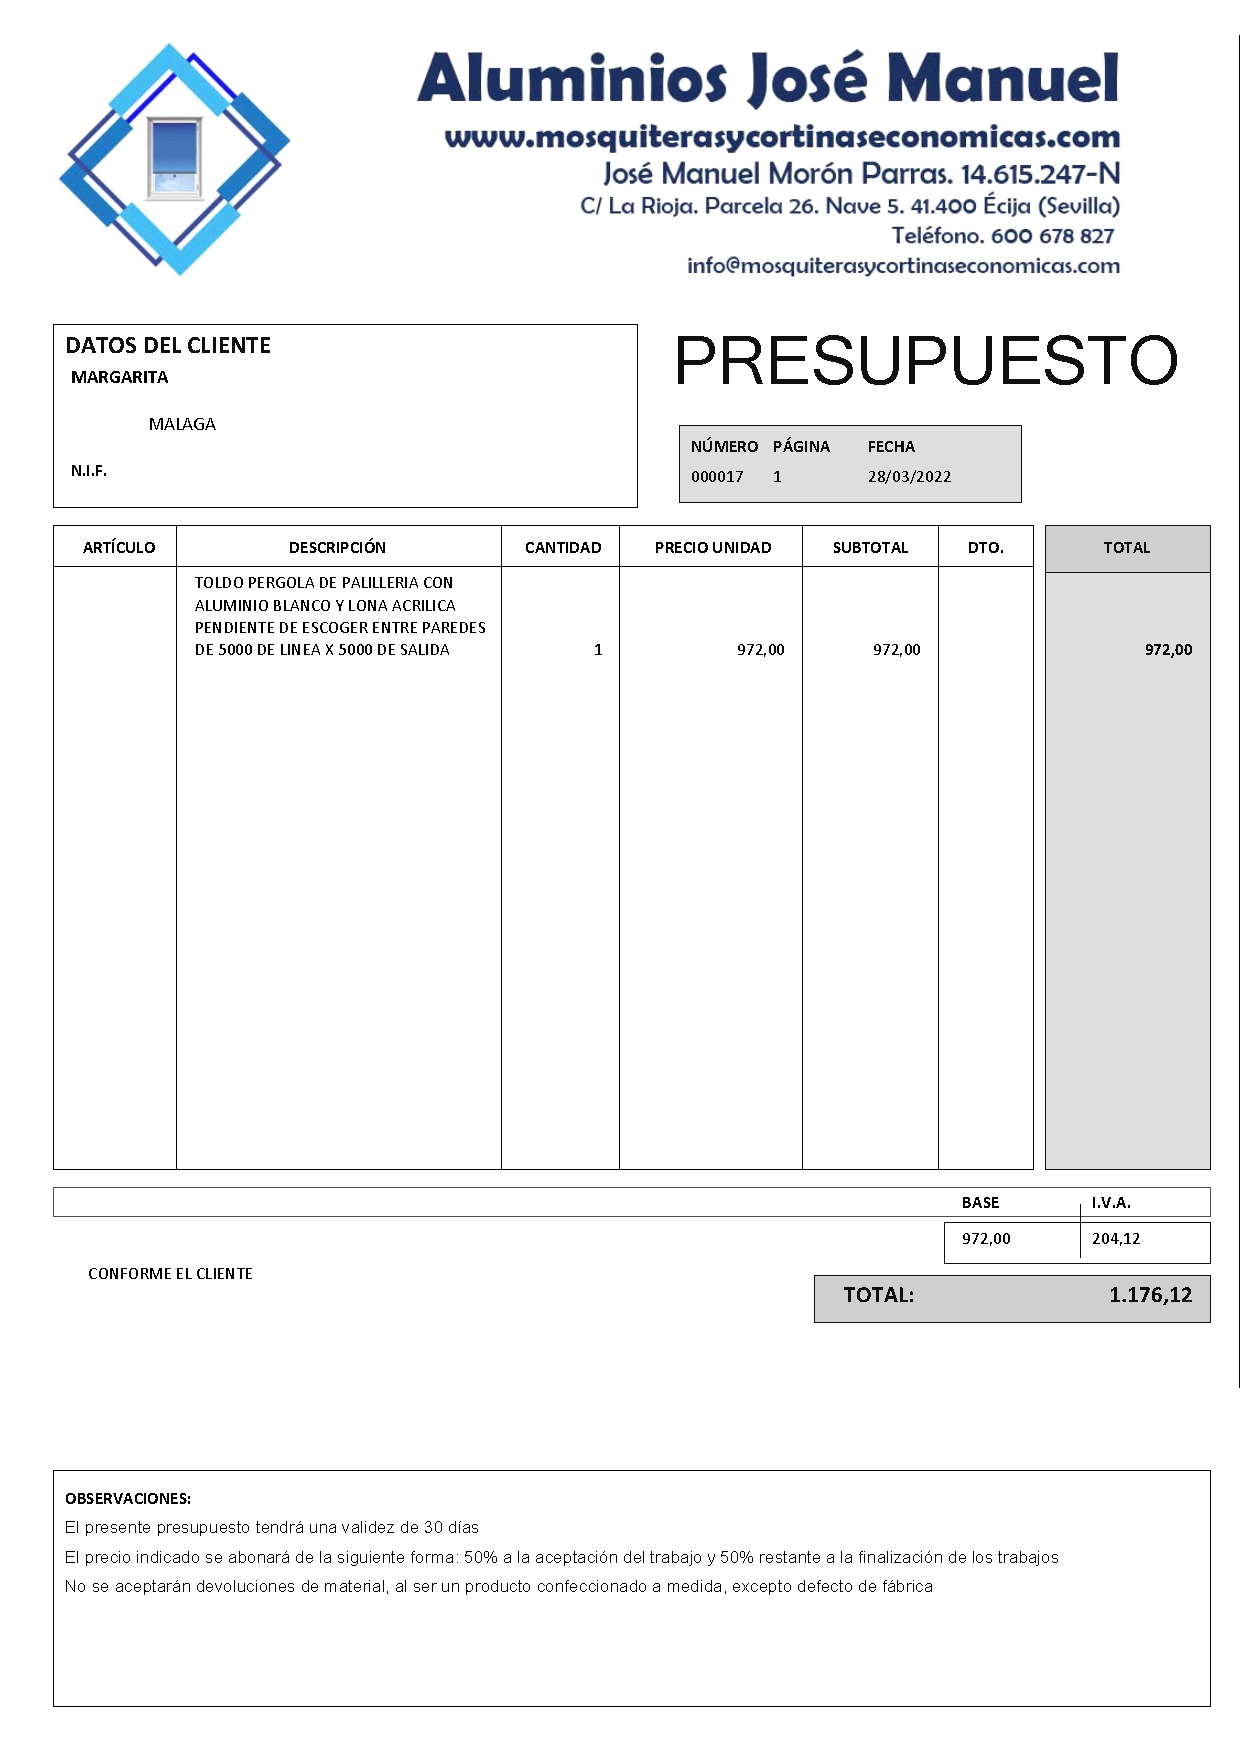
\includegraphics[scale = 0.45]{contenido/Anexos/Presupuesto 1-000017.pdf}
    \caption{Presupuesto pérgola aluminio.}
    \label{fig:PresupPA}
\end{figure}

Considerando el presupuesto que se ha obtenido y que se puede observar en la \autoref{fig:PresupPA} se puede estimar el precio medio de una pérgola como: 1176,12 \glssymbol{euro} / 25 \glssymbol{metrocuadrado} = 47,05 \glssymbol{europormetrocuadrado}. Dando un total para cada modelo de:

\begin{table}[H]
\centering
\begin{tabular}{|l|c|c|}
\hline
Vehículo                  & Área Pérgola               & Precio Total \\\hline
Askoll eS1                & 30,75 \glssymbol{metrocuadrado} & 1.446,79 \glssymbol{euro}    \\\hline
KYMCO Agility Carry 50 E5 & 24,87 \glssymbol{metrocuadrado} & 1.170,13 \glssymbol{euro}    \\\hline
KYMCO Agility Carry 125   & 17,04 \glssymbol{metrocuadrado} & 801 \glssymbol{euro}       \\\hline
F.Lli Schiano E-Moon      & 7,82 \glssymbol{metrocuadrado}  & 367,93 \glssymbol{euro}     \\\hline
Infinitron CITYJam Pro    & 9,53 \glssymbol{metrocuadrado}  & 448,39 \glssymbol{euro}    \\\hline
\end{tabular}
\caption{Precio de instalación de Pérgola para vehículos con supuesto de 5 \glssymbol{km}.}
\end{table}

\begin{table}[H]
\centering
\begin{tabular}{|l|c|c|}
\hline
Vehículo                  & Área Pérgola               & Precio Total \\\hline
Askoll eS1                & 23,92 \glssymbol{metrocuadrado} & 1.125,43 \glssymbol{euro}    \\\hline
KYMCO Agility Carry 50 E5 & 24,87 \glssymbol{metrocuadrado} & 1.170,13 \glssymbol{euro}    \\\hline
KYMCO Agility Carry 125   & 17,04 \glssymbol{metrocuadrado} & 801 \glssymbol{euro}       \\\hline
F.Lli Schiano E-Moon      & 7,82 \glssymbol{metrocuadrado}  & 367,93 \glssymbol{euro}     \\\hline
Infinitron CITYJam Pro    & 6,42 \glssymbol{metrocuadrado}  & 302,06 \glssymbol{euro}    \\\hline
\end{tabular}
\caption{Precio de instalación de Pérgola para vehículos con supuesto de 7,5 \glssymbol{km}.}
\end{table}

Para el modelo híbrido, se cuenta con con un área de parking de 10,04 \glssymbol{metrocuadrado} que equivale a un total de 489,32 \glssymbol{euro}.

\subsubsection{Cálculo del precio de la instalación de un garaje cerrado (prefabricado)}
Considerando los precios estudiados en Fixr \cite{fixrgaraje} (2000 \glssymbol{euro} para una garaje cerrado de 15 \glssymbol{europormetrocuadrado}) se puede estimar un precio medio de 133,33 \glssymbol{europormetrocuadrado}. Dando un total por modelo de:

\begin{table}[H]
\centering
\begin{tabular}{|l|c|c|}
\hline
Vehículo                  & Area Garaje                & Precio Total \\\hline
Askoll eS1                & 30,75 \glssymbol{metrocuadrado} & 4.099,90 \glssymbol{euro}    \\\hline
KYMCO Agility Carry 50 E5 & 24,87 \glssymbol{metrocuadrado} & 3.315,92 \glssymbol{euro}    \\\hline
KYMCO Agility Carry 125   & 17,04 \glssymbol{metrocuadrado} & 2.271,94 \glssymbol{euro}    \\\hline
F.Lli Schiano E-Moon      & 7,82 \glssymbol{metrocuadrado}  & 1.042,64 \glssymbol{euro}    \\\hline
Infinitron CITYJam Pro    & 9,53 \glssymbol{metrocuadrado}  & 1.270,63 \glssymbol{euro}   \\\hline
\end{tabular}
\caption{Precio de instalación de Garaje para vehículos con supuesto de 5 \glssymbol{km}.}
\end{table}

\begin{table}[H]
\centering
\begin{tabular}{|l|c|c|}
\hline
Vehículo                  & Área Garaje                & Precio Total \\\hline
Askoll eS1                & 23,92 \glssymbol{metrocuadrado} & 3.189,25 \glssymbol{euro}   \\\hline
KYMCO Agility Carry 50 E5 & 24,87 \glssymbol{metrocuadrado} & 3.315,92 \glssymbol{euro}    \\\hline
KYMCO Agility Carry 125   & 17,04 \glssymbol{metrocuadrado} & 2.271,94 \glssymbol{euro}    \\\hline
F.Lli Schiano E-Moon      & 7,82 \glssymbol{metrocuadrado}  & 1.042,64 \glssymbol{euro}    \\\hline
Infinitron CITYJam Pro    & 6,42 \glssymbol{metrocuadrado}  & 855,98 \glssymbol{euro}    \\\hline
\end{tabular}
\caption{Precio de instalación de Garaje para vehículos con supuesto de 7,5 \glssymbol{km}.}
\end{table}

Para el modelo híbrido, se cuenta con un área de parking de 10,04 \glssymbol{metrocuadrado} que equivale a un total de 1.338,63 \glssymbol{euro}.

\subsection{Cálculo del precio de la instalación eléctrica}
En caso de contar con vehículos eléctricos se debe contar con puntos de carga para estos, en este caso se debe tener en cuenta que todos los vehículos presentados cuentan con un cargador para baterías que se puede conectar directamente a una toma de corriente.

\subsubsection{Intalación eléctrica para exteriores (caso pergola)} El coste de una instalación eléctrica para exteriores, según se estima en Zaask \cite{zaaskiem} se encuentra entre 700 y 1.550 \glssymbol{euro}, puesto que necesitaríamos varias tomas y les daremos mucho uso, asumiremos el precio máximo para asegurarnos la máxima calidad posible, 1.550 \glssymbol{euro}.

\subsubsection{Instalación eléctrica para interiores (caso garaje)} Considerando que la instalación eléctrica de interior requiere menos medidas de seguridad, consideraremos que el precio de esta será siempre inferior a la instalación exterior por lo que tomaremos el punto medio de 1.000 \glssymbol{euro}.

\newpage
% \addcontentsline{toc}{section}{Referencias}
% \section*{Referencias}
% \label{referencias_nucleo}
% \makeatletter
% \def\@bibitem#1{\item\if@filesw \immediate\write\@auxout
%   {\string\bibcite{#1}{A\the\value{\@listctr}}}\fi\ignorespaces}
% \def\@biblabel#1{[A{#1}]}
% \makeatother
% \printbibheading[title={Referencias},heading=bibintoc]
\nocite{*}
\newrefcontext[labelprefix=\thesection.]
\printbibheading[title={Referencias},heading=subbibintoc]
\printbibliography[heading=none,resetnumbers=true,keyword=infraestructura]
\label{applastpage}

% \newpage
% \section{Referencias}
\printbibheading[title={Referencias},heading=bibnumbered]
\printbibliography[resetnumbers=true,keyword=nolaw,heading=none]
% \printbibliography[keyword=nolaw, title={Books}]
% CONTENIDO. BIBLIOGRAFÍA.
%%%%
%\nocite{*} %incluye TODOS los documentos de la base de datos bibliográfica sean o no citados en el texto
% \bibliographystyle{unsrt}

% \begingroup
% \renewcommand{\section}[2]{}%
% %\renewcommand{\chapter}[2]{}% for other classes
% \bibliography{bibliografia}
% \endgroup


\end{appendices}

\begin{table}[H]
    \centering
\renewcommand{\arraystretch}{4.5}
\resizebox{\textwidth}{!}{%
\begin{tabular}{|l|lllllll|} \hline
\multicolumn{1}{|l}{\begin{tabular}[c]{@{}l@{}}\\\end{tabular}} &  &  &  &  &  &  &  \\
\multicolumn{1}{|}{} & \multirow{4}{*}{} & \multicolumn{5}{l}{Documento \identificadorx} &  \\
\multicolumn{1}{|l}{} &  & \multicolumn{5}{l}{Hoja de datos} &  \\
\multicolumn{1}{|l}{} &  & \multicolumn{2}{l}{Datos de emisión} & \multicolumn{3}{l}{Proyecto No. 1} &  \\
\multicolumn{1}{|l}{} &  & \multicolumn{2}{l}{30 de febrero del 2022} & \multicolumn{3}{l}{\shortstack[l]{\organizacionx}.} &  \\ \cline{2-7}
 & \multicolumn{1}{l|}{} & \multicolumn{5}{l|}{\shortstack[l]{\organizacionx}} &  \\ \cline{2-7}
 & \multicolumn{6}{l|}{\shortstack[l]{\textbf{Título}\\\titulox}} &  \\ \cline{2-7}
 & \multicolumn{6}{l|}{\shortstack[l]{\textbf{Autores}\\
Lucas Acebal Colli\\Alberto Cándido Amores Navas\\Carlos Atencia Tabares\\Jorge Luis Benavides Macías\\Irene Guijarro Molina}
} &  \\ \cline{2-7}
 & \multicolumn{6}{l|}{\multirow{2}{*}{\shortstack[l]{\textbf{Resumen}\\
En este informe técnico se estudian las posibles opciones de vehículos para incorporar un servicio de reparto a domicilio para la empresa \\ \textit{DELICIOUS BURGER S.A.}, en la que se presentan diferentes opciones de vehículos de gasolina y eléctricos. El objetivo es encontrar  la solución \\ más eficiente económicamente para poder satisfacer las necesidades del servicio.  Se realizará un estudio del mercado  y se escogerán las opciones \\ con mejor relación calidad/precio,  realizando una comparación entre estas para posteriormente poder escoger la opción más eficiente. Se podrá \\ observar que la mejor opción es la eléctrica, considerando  una flota de 2 motocicletas y 7 patinetes eléctricos para el reparto, junto con la \\ construcción de un garaje prefabricado y la instalación eléctrica para la carga de las baterías.}}} &  \\
 & \multicolumn{6}{l|}{} &  \\ \cline{2-7}
 & \multicolumn{6}{l|}{\shortstack[l]{\textbf{Palabras claves}\\
 Vehículos, eléctrico, análisis, reparto, comida, infraestructura.}} &  \\ \cline{2-7}
 & \multicolumn{6}{l|}{} &  \\ \cline{2-7}
 & \multicolumn{6}{l|}{} &  \\ \cline{2-7}
 & \multicolumn{4}{l|}{\multirow{2}{*}{}} & \multicolumn{2}{l|}{} &  \\ \cline{6-7}
 & \multicolumn{4}{l|}{\shortstack[l]{\textbf{Lista de distribución}\\ 
 - Buendía Cisma Gonzalez (DNI 98899898X) \\
 - D. Leopoldo Juantegui Pujals (DNI 12349876G)}} & \multicolumn{2}{l|}{} &  \\ \cline{2-7}
 & \multicolumn{1}{l|}{\shortstack[l]{\textbf{Seguridad}\\\seguridadx}} & \multicolumn{3}{l|}{\shortstack[l]{\textbf{Idioma}\\Español}} & \multicolumn{1}{l|}{\shortstack[l]{\textbf{N.º páginas}\\\thepage \ páginas}} & \multicolumn{1}{l|}{\shortstack[l]{\textbf{N.º de copias}\\0 copias}} &  \\ \cline{2-7}
 & \multicolumn{1}{l|}{\multirow{2}{*}{\shortstack[l]{\textbf{Asosciacion}\\\asociacionx}}} & \multicolumn{5}{l|}{\multirow{3}{*}{}} &  \\
 & \multicolumn{1}{l|}{} & \multicolumn{5}{l|}{} &  \\ \cline{2-2}
 & \multicolumn{1}{l|}{} & \multicolumn{5}{l|}{} &  \\ \cline{2-7}
\multicolumn{1}{|l}{} &  &  &  &  &  &  &  \\ \hline
\end{tabular}
}
\end{table}
\newpage
\ihead{\seguridadx}
\ohead{\identificadorx}
\vspace*{\fill}
\begin{center}
\huge{CONFIDENCIAL}    
\end{center}
\vspace*{\fill}
\input{include/portada/cubierta_posterior}

% Hoja de datos
% Cubierta posterior
\end{document}
